\documentclass[12pt]{article}

\usepackage{geometry}
\geometry{
 a4paper,
 papersize={210mm,297mm},
 total={165mm,257mm},
 top=20mm,
 left=30mm
 }
\usepackage{graphicx}

\usepackage[utf8]{inputenc}
\usepackage[english,russian]{babel}
\usepackage[12pt]{extsizes}
\usepackage{hyperref}
\usepackage{amsmath}
\usepackage{amsthm}
\usepackage{amsfonts}
\usepackage{dsfont} % for indicator
\usepackage{amssymb}
\usepackage{mathtools}
\usepackage{cite}
\usepackage[nottoc,numbib]{tocbibind}
\usepackage[font=small]{caption}
\usepackage{subcaption}

\usepackage{booktabs}       % professional-quality tables
\usepackage{amsfonts}       % blackboard math symbols
\usepackage{nicefrac}       % compact symbols for 1/2, etc.
\usepackage{microtype}      % microtypography
\usepackage{float}

\usepackage{multirow, array}
\setlength{\parindent}{5ex}

% \usepackage{mathptmx}
% \DeclareMathSizes{14}{16}{12}{10}

\hypersetup{
    colorlinks=true,
    linkcolor=black,
    filecolor=magenta,      
    urlcolor=red,
}

%\usepackage{fullpage}
\renewcommand{\baselinestretch}{2}
\makeatletter
\renewcommand\@biblabel[1]{#1.}
\makeatother

\begin{document}
    \pagenumbering{arabic}
    \tableofcontents
    \newpage

\section*{ВВЕДЕНИЕ}
    \label{sec:intro}
    \addcontentsline{toc}{section}{\nameref{sec:intro}}
\subsection*{Парная игра}
    Мы изучаем пространственную игру, основанную на дилемме заключенного. Два игрока, играя друг против друга, могут либо кооперировать(кооператор, $\mathcal{C}$), либо предавать(дефектор, $\mathcal{D}$).
        
    Если оба игрока — кооператоры, то каждый получает условный выигрыш $1$. Если один из них дефектор, а другой кооператор, то первый получает выигрыш в $b>1$ раз больше, чем при игре $\mathcal{C}-\mathcal{C}$, а последний ничего не получает, как и при игре двух дефекторов(таблица \ref{table:gametable}). 
    
    Затем агенты выбирают тактику, принесшую наибольший выигрыш, после чего игра повторяется.
    При такой игре 1 на 1 оптимальной тактикой будет $\mathcal{D}$(если изначально хотя бы один из агентов был дефектором, то при игре против кооператора он получает больший выигрыш($b>1$) и кооператор становится дефектором)(объяснение можно найти в секции 2 \textit{The prisoner’s dilemma} статьи \cite{NACHBAR1992307})

    \begin{table}[h!]\centering
        \begin{tabular}{cc|c|c|}
              & \multicolumn{1}{c}{} & \multicolumn{2}{c}{Агент}\\
              & \multicolumn{1}{c}{} & \multicolumn{1}{c}{$\mathcal{D}$}  & \multicolumn{1}{c}{$\mathcal{C}$} \\\cline{3-4}
              {Сосед}  & $\mathcal{D}$ & $0$ & $0$ \\\cline{3-4}
              & $\mathcal{C}$ & $b$ & $1$ \\\cline{3-4}
        \end{tabular}
        \caption{Таблица выигрышей при стандартной игре}
        \label{table:gametable}
    \end{table}

\subsection*{Игра на сетке}
    Рассмотрим дилемму заключенного на квадратной сетке $L\times L$ с $L^2$ агентами. Каждый попарно взаимодействует одновременно с 8 соседями, после чего среди себя и своих соседей выбирает поведение(кооперировать или предавать), принесшее наибольший выигрыш на текущем ходу(агенты не имеют памяти, поэтому максимизируют выигрыш здесь и сейчас). Выигрыш агента является суммой выигрышей игр с соседями.

\subsection*{Игра Новака-Мэя}
    М.Новак и Р.Мэй\cite{NOWAK1992,NOWAK1993} исследовали поведение пространственной игры с учётом взаимодействия агента с самим собой.\footnote{Такая модификация игры позволяет каждому агенту представлять группу организмов или молекул, внутри которой могут происходить взаимодействия.} Те выигрыш игрока $q$ может быть рассчитан как
    \begin{equation*}
        P_q = n(\mathds{1}_{\mathcal{C}}(q)(1-b) + b) + \mathds{1}_{\mathcal{C}}(q)
    \end{equation*}
        
    Устанавливая начальную конфигурацию  игрового поля симметричной, М.Новак и Р.Мэй наблюдали за поведением системы на квадратной решётке после достижения ею стационарного состояния.
    
    Исследование было продолжено С.Колотевым, А.Малютиным, Е.Буровским, С.Крашаковым и Л.Щуром \cite{KOLOTEV2018}. В их статье было рассмотрено поведение игры при разных размерах поля и параметрах выигрыша. Аналогичные исследования были проведены и на треугольной решётке, и сравнительный анализ игр на двух типах решётки был опубликован в \cite{sq_and_tr}. Как оказалось, поведение игры зависит от типа поля, т.е. локальная структура связей между игроками-соседями определяет всю систему.
 
\section{Среднее поле}
    \begin{table}[h!]\centering
        \begin{tabular}{cc|c|c|}
              & \multicolumn{1}{c}{} & \multicolumn{2}{c}{Агент}\\
              & \multicolumn{1}{c}{} & \multicolumn{1}{c}{$\mathcal{D}$}  & \multicolumn{1}{c}{$\mathcal{C}$} \\\cline{3-4}
              {Сосед}  & $\mathcal{D}$ & $0$ & $0$ \\\cline{3-4}
              & $\mathcal{C}$ & $bf_c$ & $f_c$ \\\cline{3-4}
        \end{tabular}
        \caption{Таблица выигрышей при игре против среднего поля}
        \label{table:gametable2}
    \end{table}
    Мы рассматриваем случай, когда вместо игры с самим собой агент играет против “среднего поля”: он взаимодействует с кооператором, после чего выигрыш умножается на плотность кооператоров $f_c$.(Таблица \ref{table:gametable2}) При такой модификации у агента появляется внешний источник информации о состоянии среды, в которой он находится.

\subsection{При каких значения меняется динамика игры?}
    Рассмотрим агента с некоторой стратегией. Если он и все его соседи кооператоры или дефекторы, то его поведение никак не изменится на следующем ходу и рассматривать этот случай не имеет смысла. В противном случае стратегия на следующем ходу определяется максимальным выигрышем кооператора($P_{\mathcal{C}}$) и дефектора($P_{\mathcal{D}}$), расположение которых показано на рисунке \ref{fig:neigh}.
    \begin{figure}[h!]
        \centering
        \captionsetup{justification=centering}
        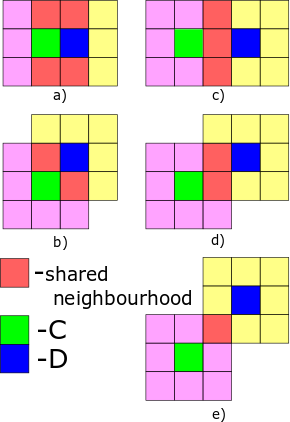
\includegraphics[scale=.5]{neighbourhoods.png}
        \caption{\small Взаимное расположение кооператоров(зеленый) и дефекторов(синий).\\
        Розовым, зеленым и желтым показаны агенты-соседи кооператора, дефектора и общие соответственно.}
        \label{fig:neigh}
    \end{figure}

    Выигрыш кооператора и дефектора можно рассчитать по формулам \eqref{eq:cooprofit} и \eqref{eq:defprofit}
    \begin{align}
        P_{\mathcal{C}}& = n_\mathrm{shared} + n_c + f_c\label{eq:cooprofit}\\
        P_{\mathcal{D}}& = b(n_\mathrm{shared} + n_d) + bf_c\label{eq:defprofit}
    \end{align}
    где
    \begin{align*}
        n_\mathrm{shared}&\text{ -- количество общих кооператоров}\\
        n_c&\text{ -- количество кооператоров-соседей кооператора}\\
        n_d&\text{ -- количество кооператоров-соседей дефектора}\\ f_c&\text{ -- плотность кооператоров на данном ходе}
    \end{align*}

    Замечание: В случаях $a$ и $b$ на рис. \ref{fig:neigh} кооператор, отмеченный зеленым, учитывается в $n_d$.
    
    Оба выигрыша равны нулю только в том случае, если на игровом полем нет кооператоров($f_c=0$), но в этом случае поле не меняется, поэтому мы его не берем во внимание.
    
    Рассмотрим максимальные $P_{\mathcal{C}}$ и $P_{\mathcal{D}}$ среди соседей и агента. Если $P_{\mathcal{C}}>P_{\mathcal{D}}$, то на следующем ходу агент будет играть как кооператор, иначе, если $P_{\mathcal{C}}<P_{\mathcal{D}}$, как дефектор. Смена стратегии, которую выбирает агент, происходит при $P_{\mathcal{C}}=P_{\mathcal{D}}$.
    \begin{equation}
    \label{eq:equalprofit}
        n_\mathrm{shared} + n_c + f_c = b(n_\mathrm{shared} + n_d) + bf_c\\
    \end{equation}

    Так как $P_{\mathcal{D}}\neq0$, то из \eqref{eq:equalprofit} получаем

    \begin{equation}
        \label{eq:transitions}
        b=\frac{n_\mathrm{shared} + n_c + f_c}{n_\mathrm{shared} + n_d + f_c}
    \end{equation}
    Для упрощения формулы введем обозначение $m=n_\mathrm{shared} + n_c$ и $n=n_\mathrm{shared} + n_d$ и позволим им не зависть друг от друга. Получаем
    \begin{equation*}
        \label{eq:transitions2}
        b=\frac{m + f_c}{n + f_c}
    \end{equation*}
    где $m,\;n=0,\dots,8$

\section{Квадратная решетка}
\subsection{Результаты моделирования}
    На рис. \ref{fig:payoffvsdensity} представлена зависимость средней плотности от выигрыша. В отличие от игры Новака-Мэя, в которой плотность кооператоров меняется скачком\cite{KOLOTEV2018}, в игре со "средним полем" она может меняться непрерывно.
    \begin{figure}[!h]
        \centering
        \captionsetup{justification=centering}
        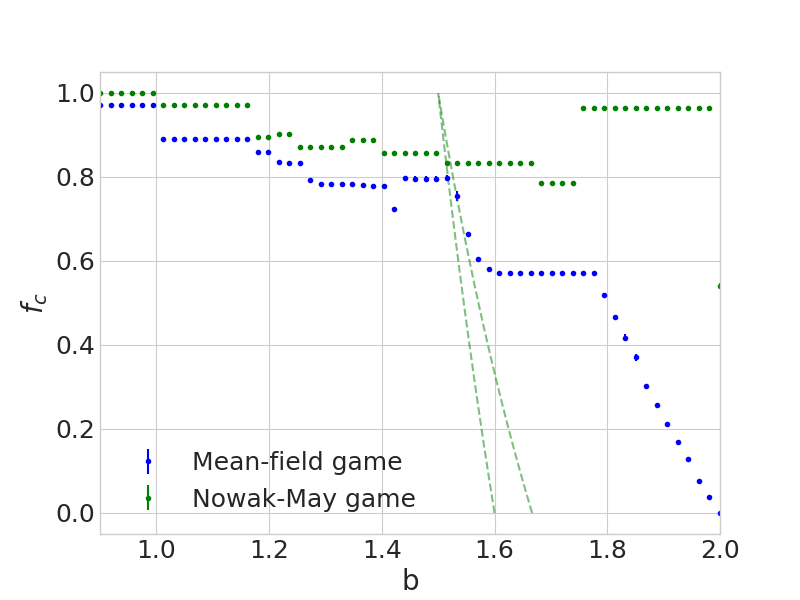
\includegraphics[width=\textwidth]{MeanFieldGame/density_NovakMay_Mean_game.png}
        \caption{Зависимость средней плотности кооператоров от выигрыша со среднеквадратичным отклонением, рассчитанная на основе 40 случайных реализация начальных условий на поле $200\times200$ с начальной плотностью $0.9$.\\
        Плотность для каждой игры рассчитана как среднее 8000 шагов после отбрасывания 10000 шагов. 
        }
        \label{fig:payoffvsdensity}
    \end{figure}

    При $b < 1.53$ дефекторы образуют статические структуры, напоминающие дендриты(рис. \ref{fig:sub1},\ref{fig:sub2},\ref{fig:sub3},\ref{fig:sub4}). С ростом параметра выигрыша ширина “каналов” увеличивается.

    Когда $1.53<b<1.6$ средняя плотность кооператоров уменьшается и "следует" за прямой, проходящей через точки $1.5$ и $1.6$, кластеры кооператоров начинают "перемещаться" по полю(рис. \ref{fig:sub5}). Кластеры кооператоров растут и уменьшаются непрерывно.

    При $1.6<b<1.62$ кооператоры начинают образовывать кластеры с прямыми линиями и прямыми углами(рис. \ref{fig:sub6}), но не могут образовать полноценные прямоугольники, так как разные кластеры сталкиваются друг с другом и "разрушаются".

    При больших b кооператоры группируются в кластеры прямоугольной формы, размеры которых уменьшаются с ростом выигрыша.(рис. \ref{fig:sub7},\ref{fig:sub8},\ref{fig:sub9})

    \begin{figure}[!htbp]
        \centering
        \captionsetup{justification=centering}
        \begin{subfigure}{.33\textwidth}
          \centering
          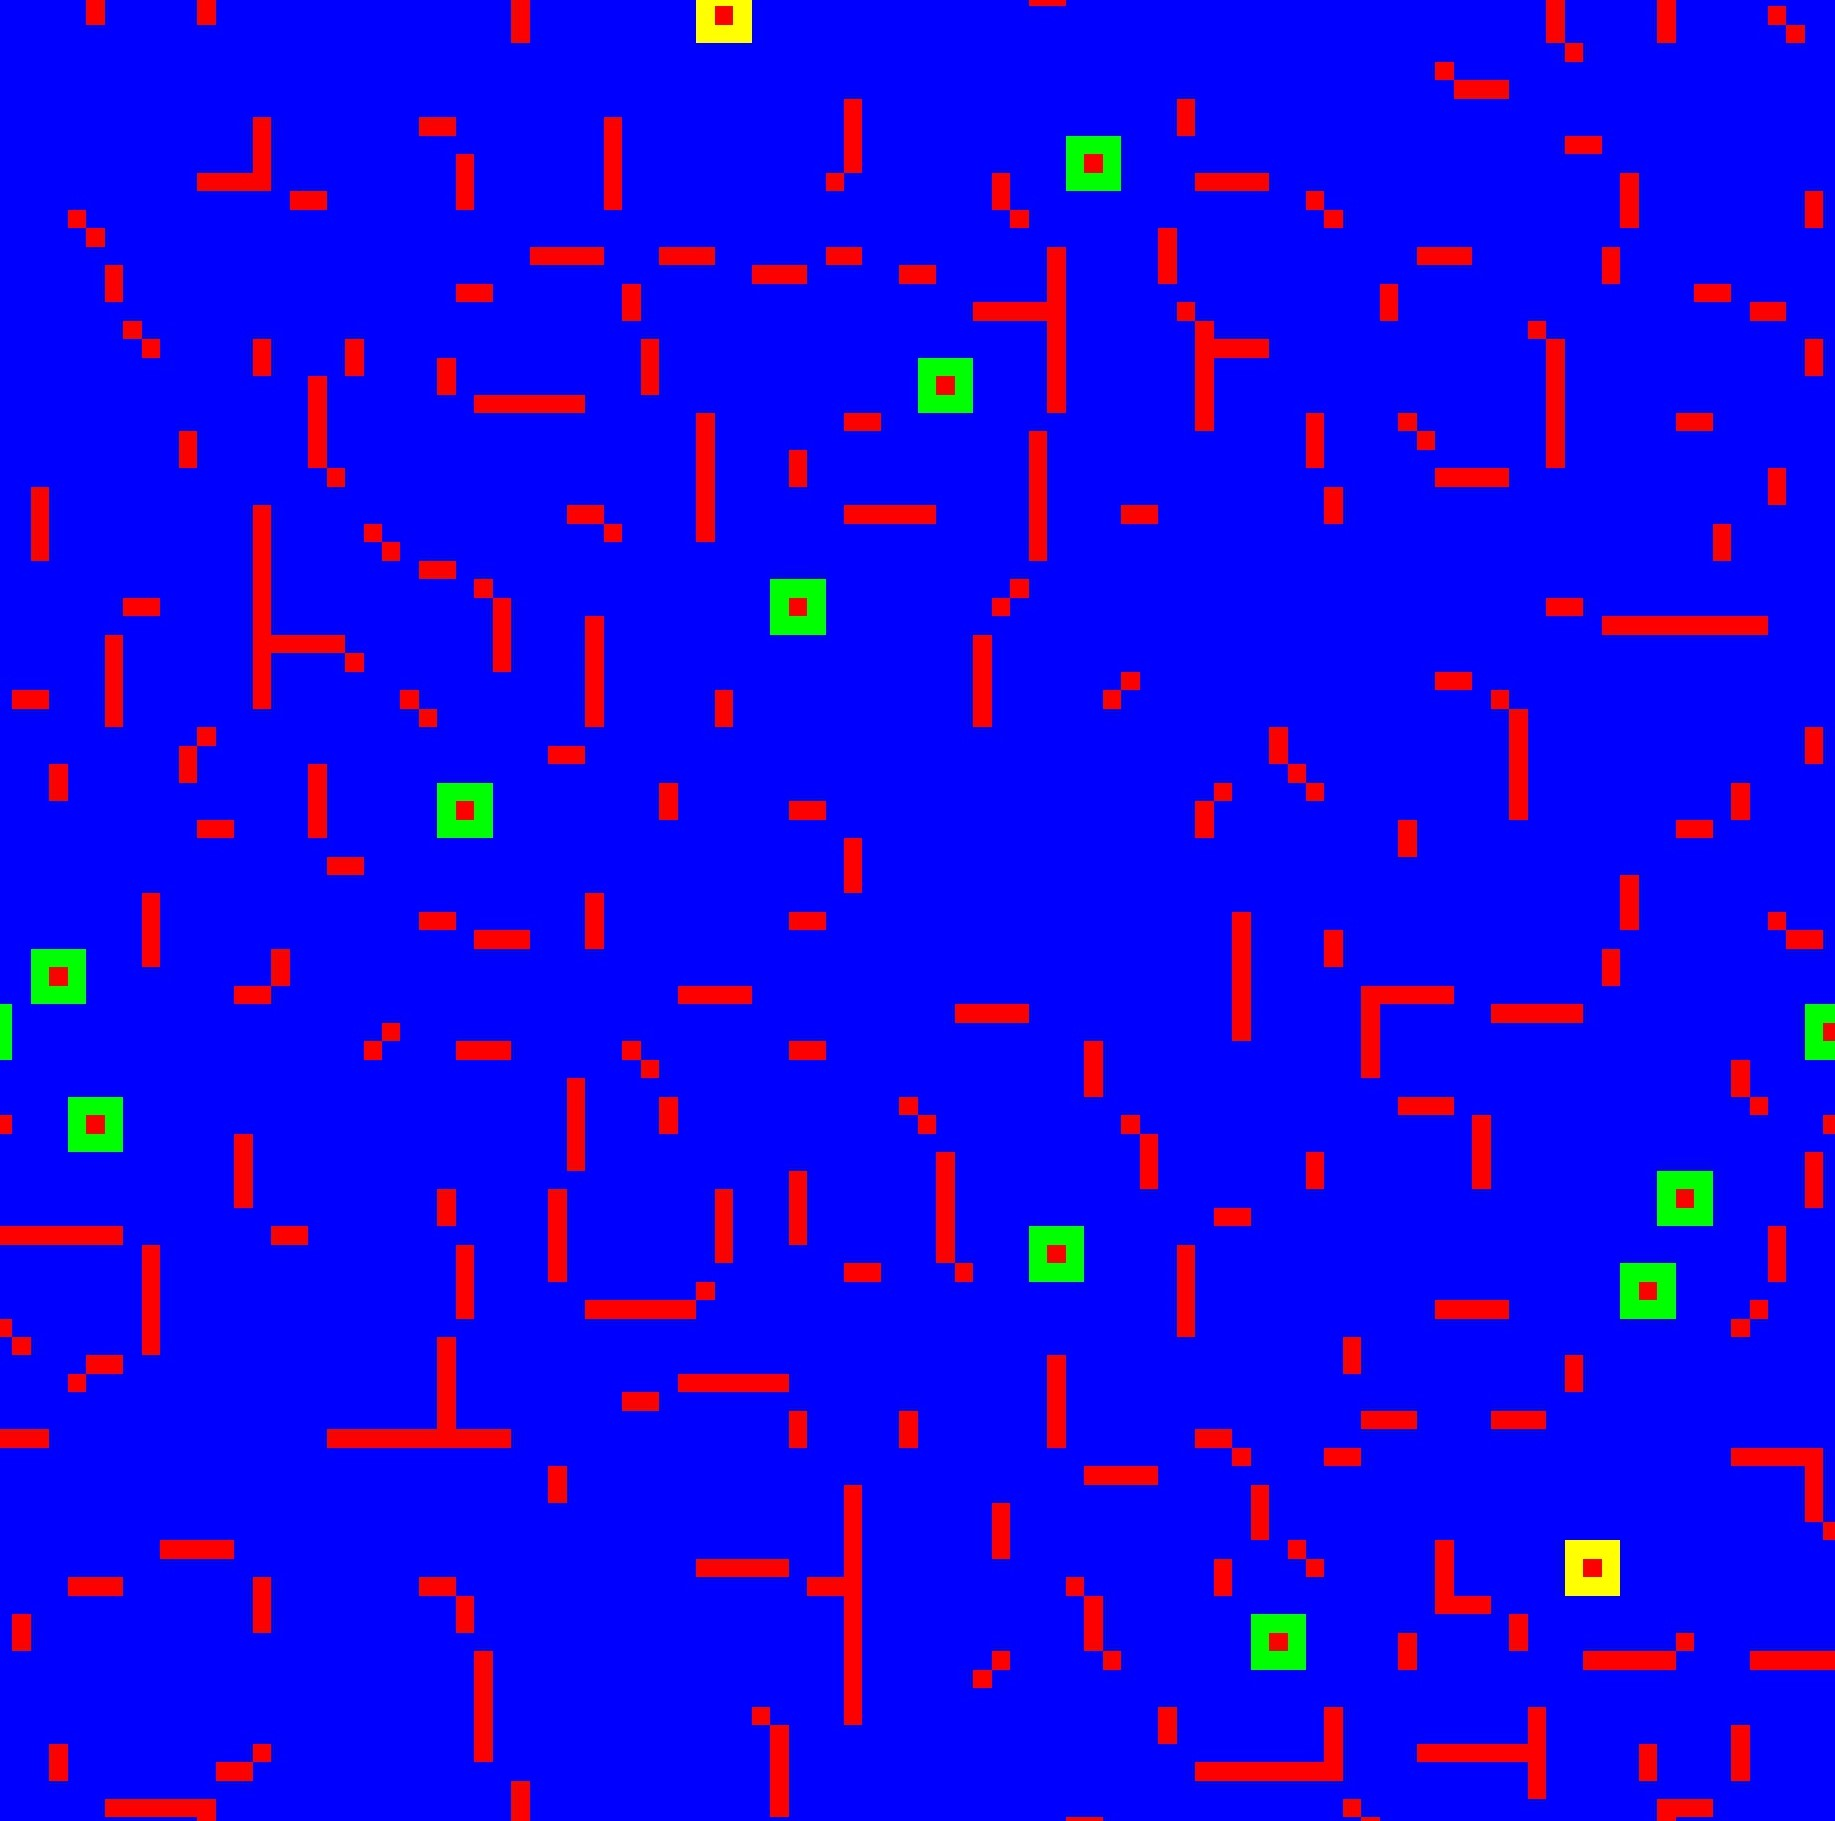
\includegraphics[width=.9\linewidth]{MeanFieldGame/snapshot_b=11.jpg}
          \caption{$b=1.1$}
          \label{fig:sub1}
        \end{subfigure}%
        \begin{subfigure}{.33\textwidth}
          \centering
          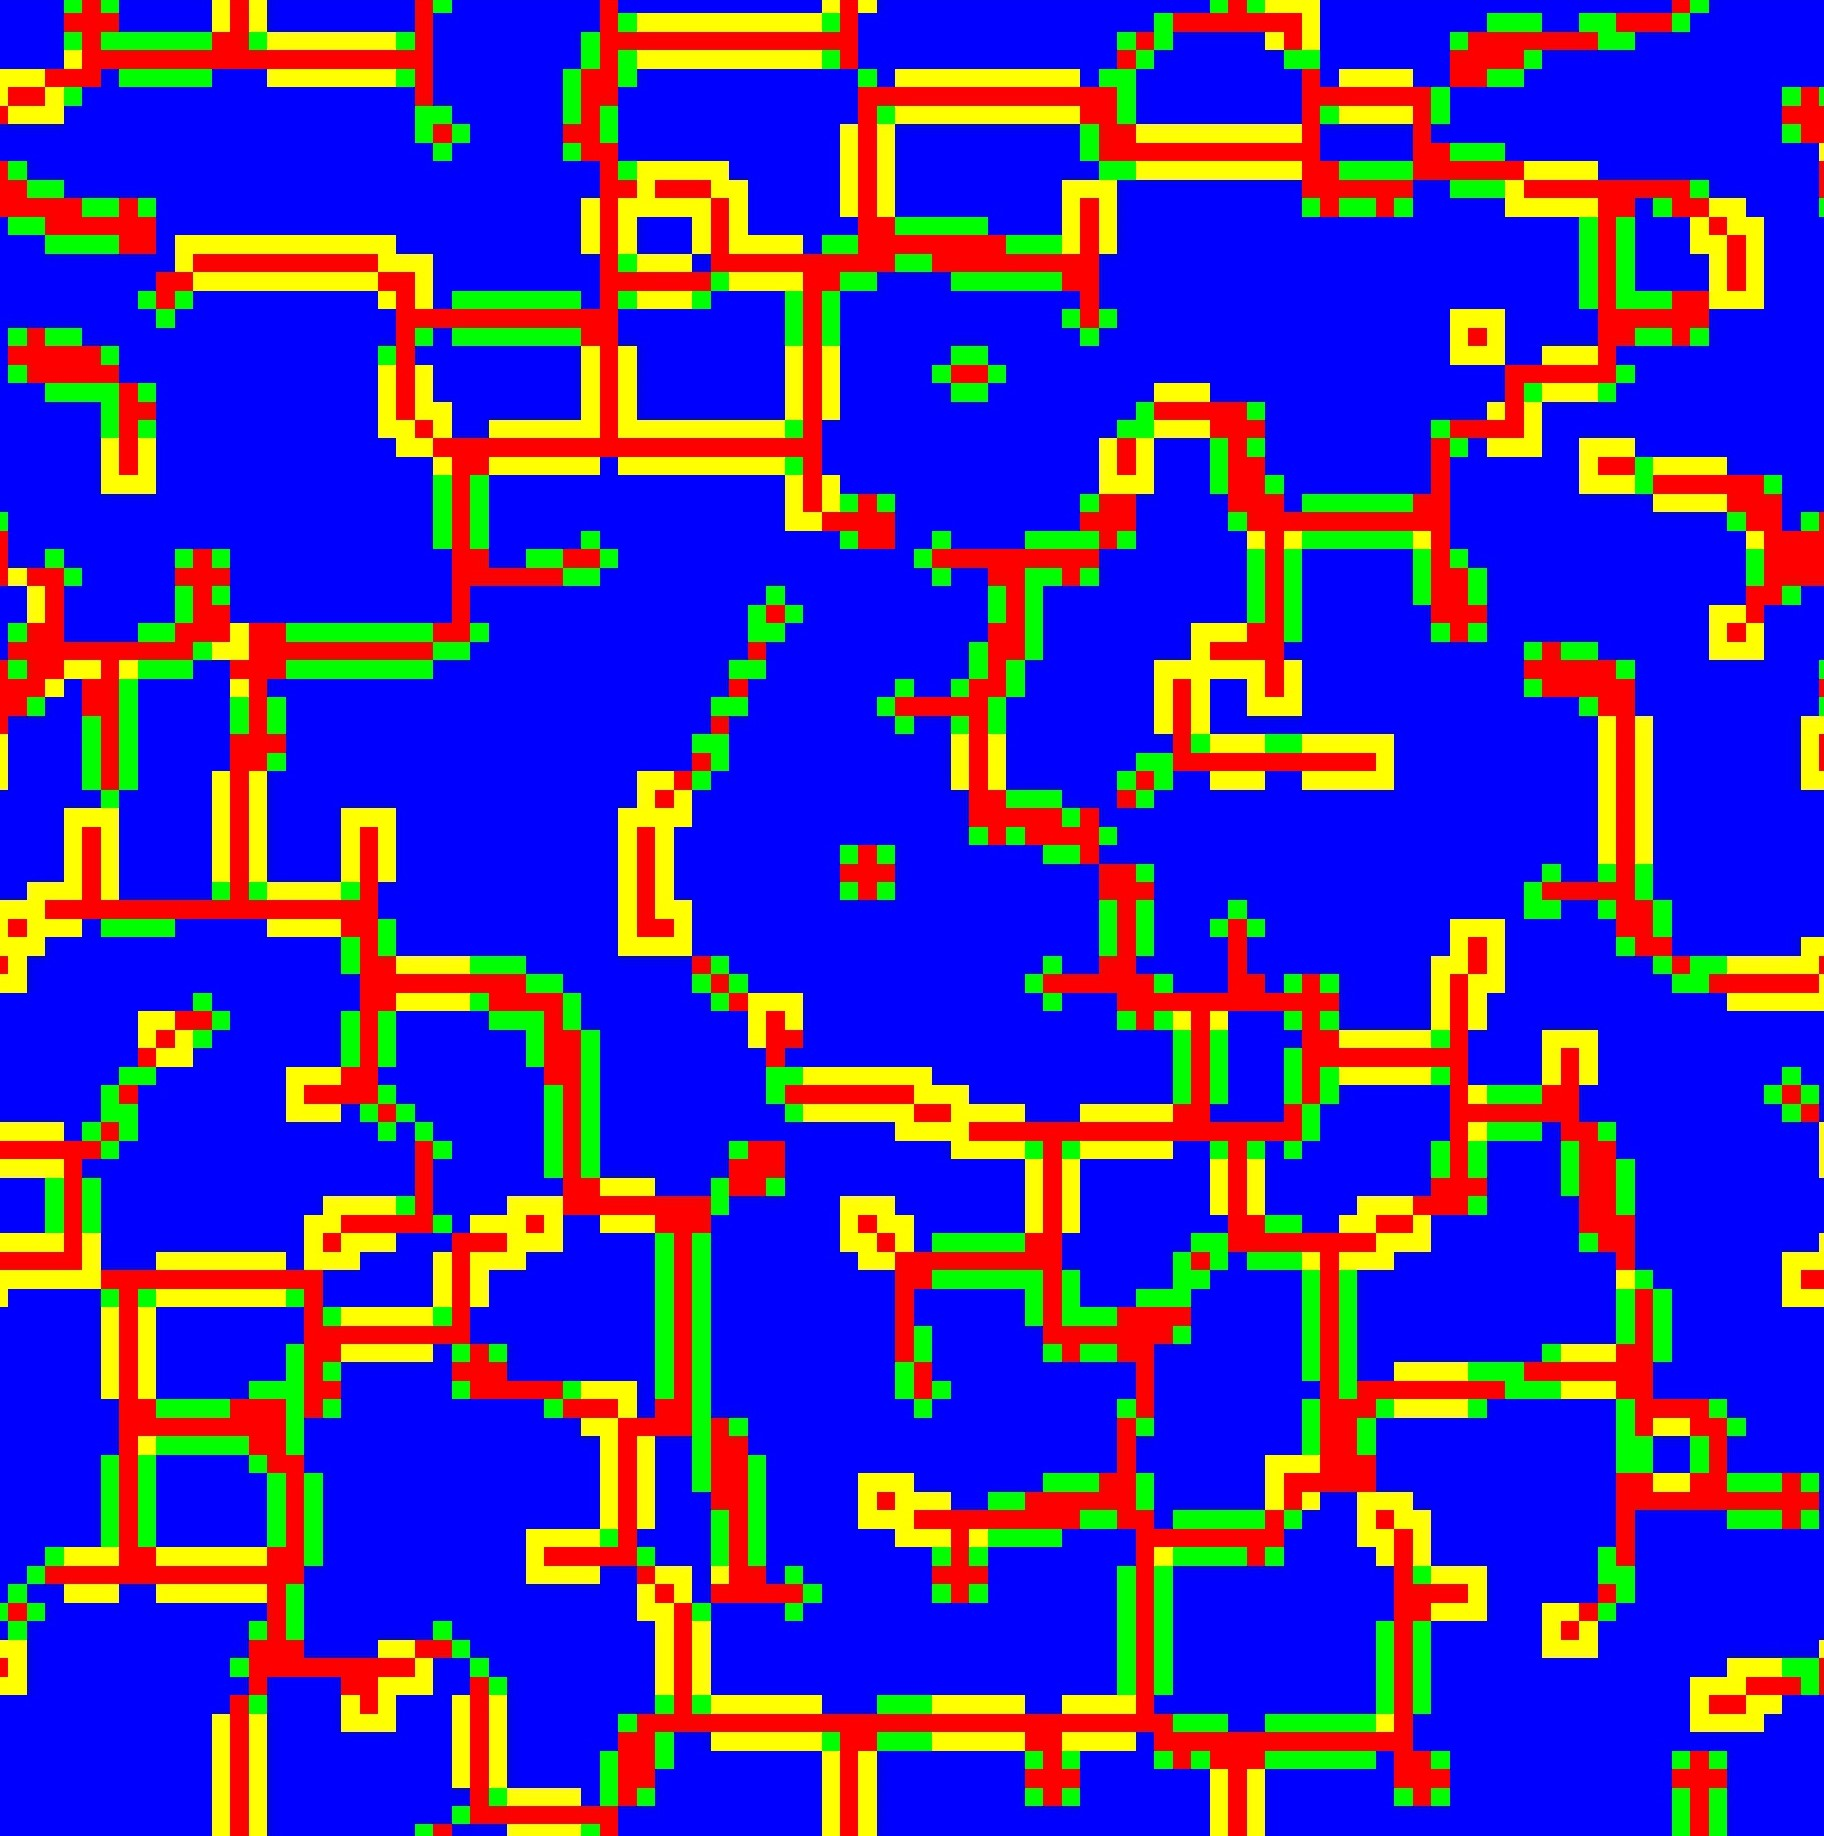
\includegraphics[width=.9\linewidth]{MeanFieldGame/snapshot_b=13.jpg}
          \caption{$b=1.3$}
          \label{fig:sub2}
        \end{subfigure}%
        \begin{subfigure}{.33\textwidth}
          \centering
          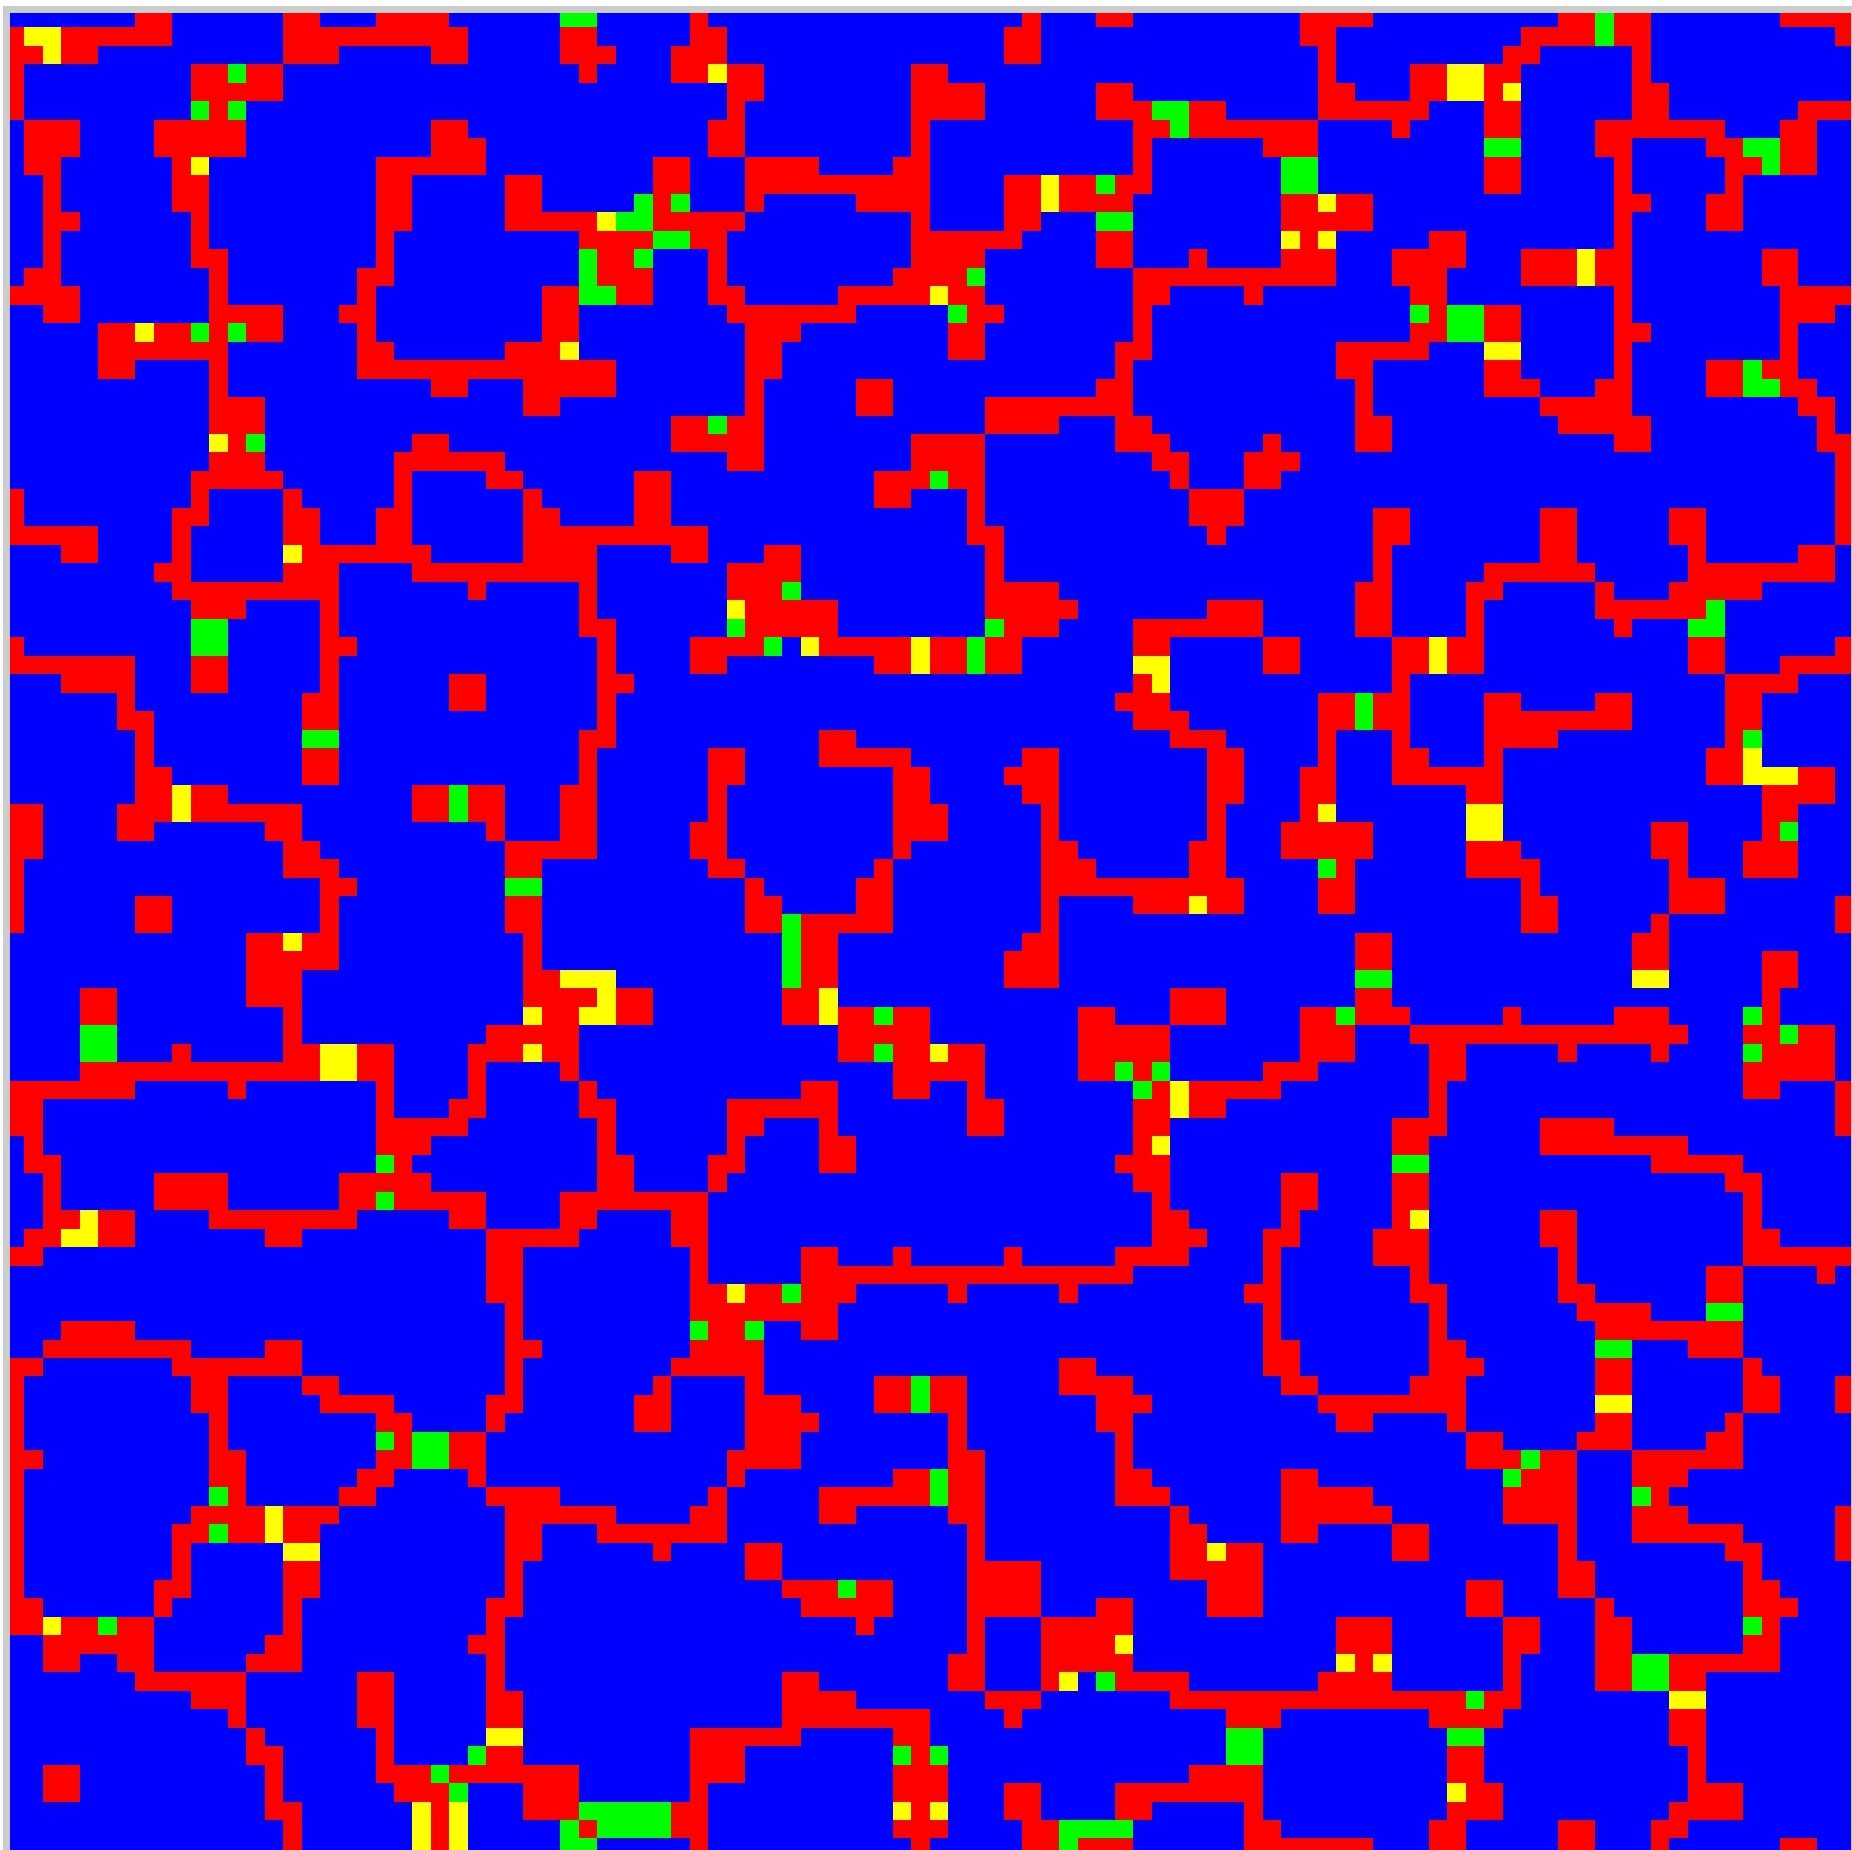
\includegraphics[width=.9\linewidth]{MeanFieldGame/snapshot_b=15.jpg}
          \caption{$b=1.5$}
          \label{fig:sub3}
        \end{subfigure}
        
        \begin{subfigure}{.33\textwidth}
          \centering
          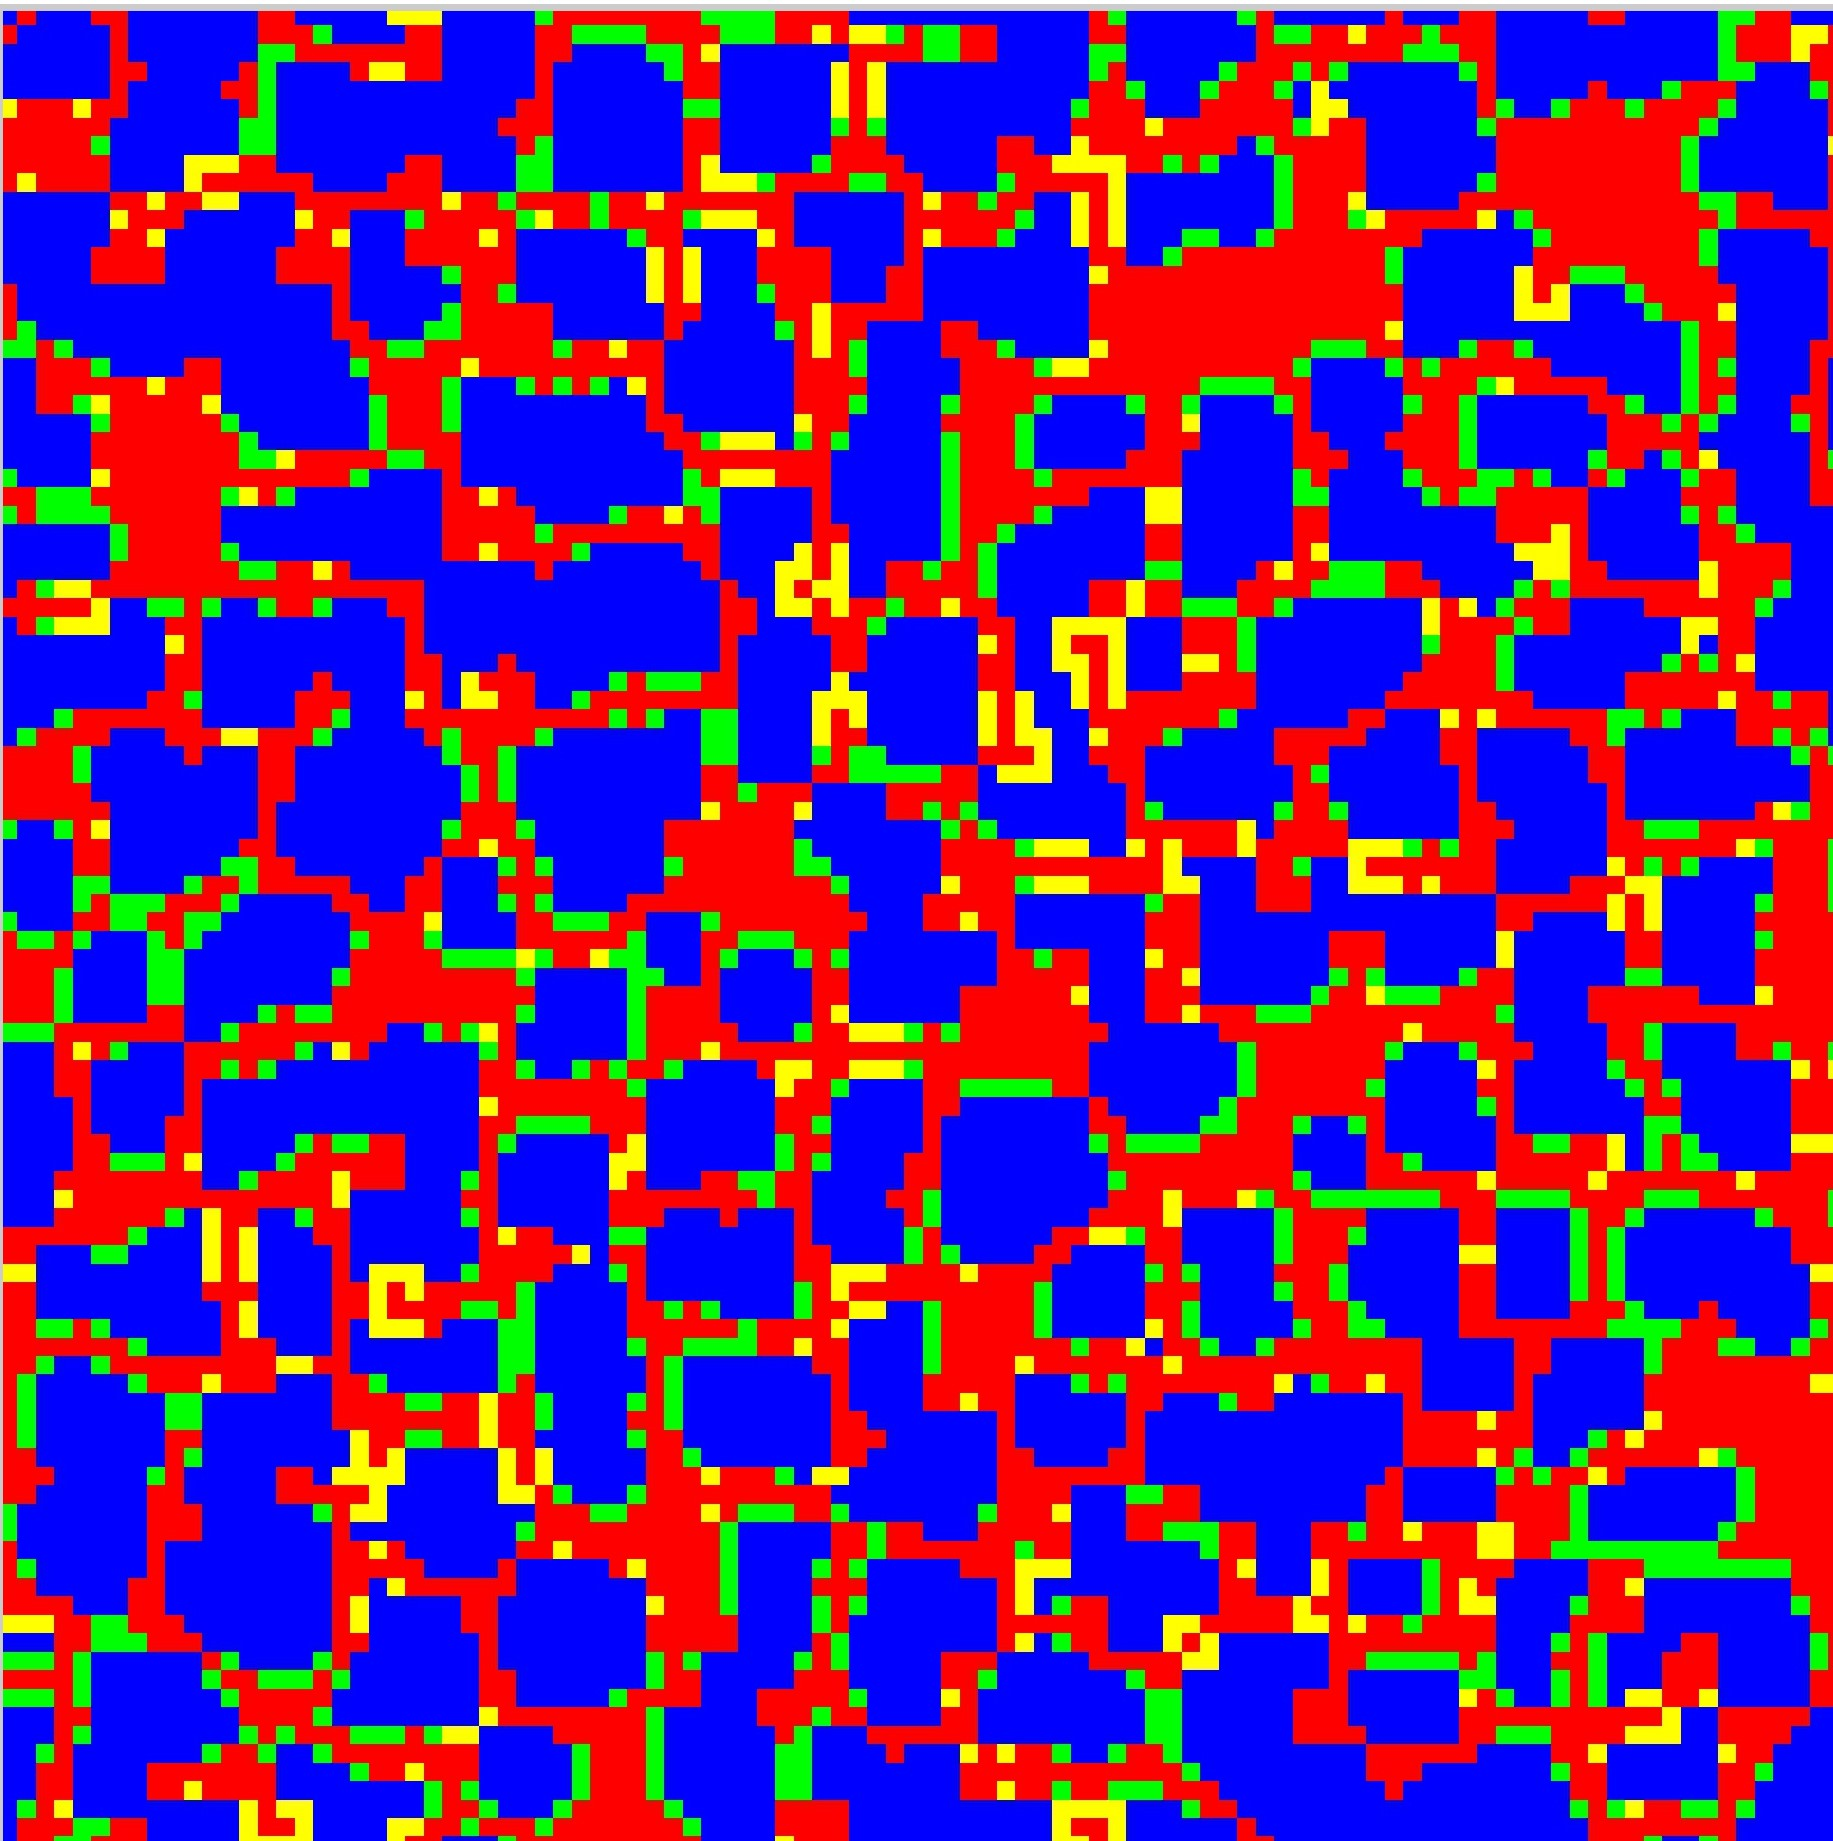
\includegraphics[width=.9\linewidth]{MeanFieldGame/snapshot_b=153.jpg}
          \caption{$b=1.53$}
          \label{fig:sub4}
        \end{subfigure}%
        \begin{subfigure}{.33\textwidth}
          \centering
          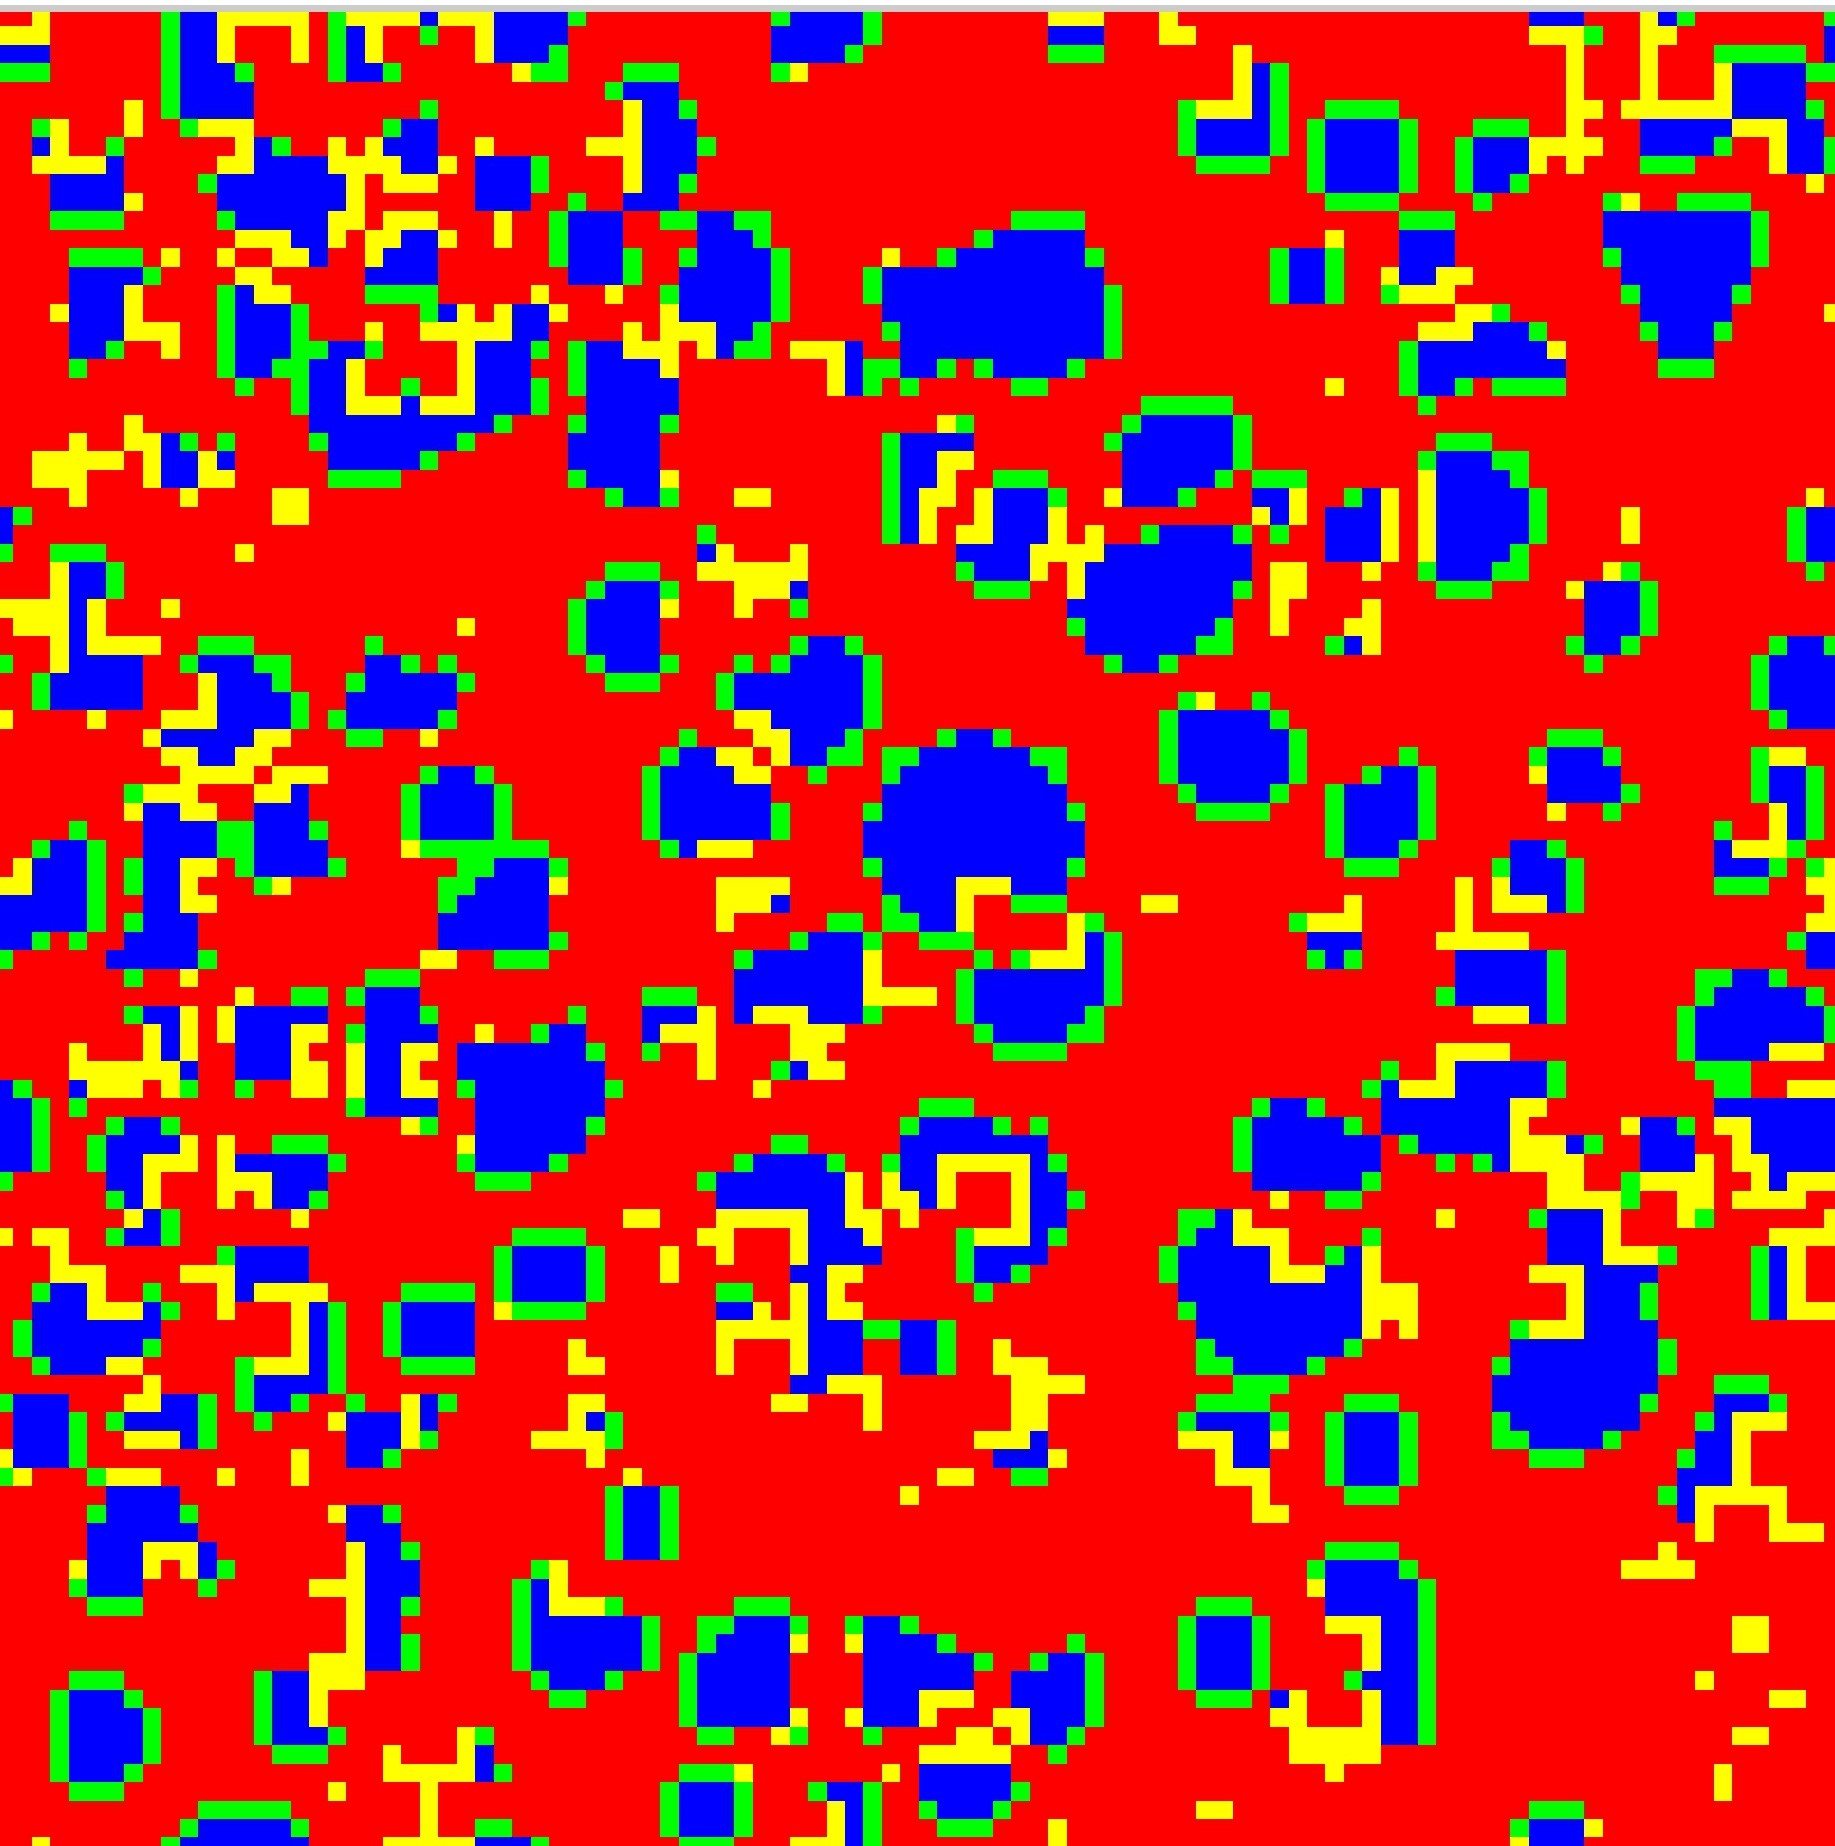
\includegraphics[width=.9\linewidth]{MeanFieldGame/snapshot_b=157.jpg}
          \caption{$b=1.57$}
          \label{fig:sub5}
        \end{subfigure}%
        \begin{subfigure}{.33\textwidth}
          \centering
          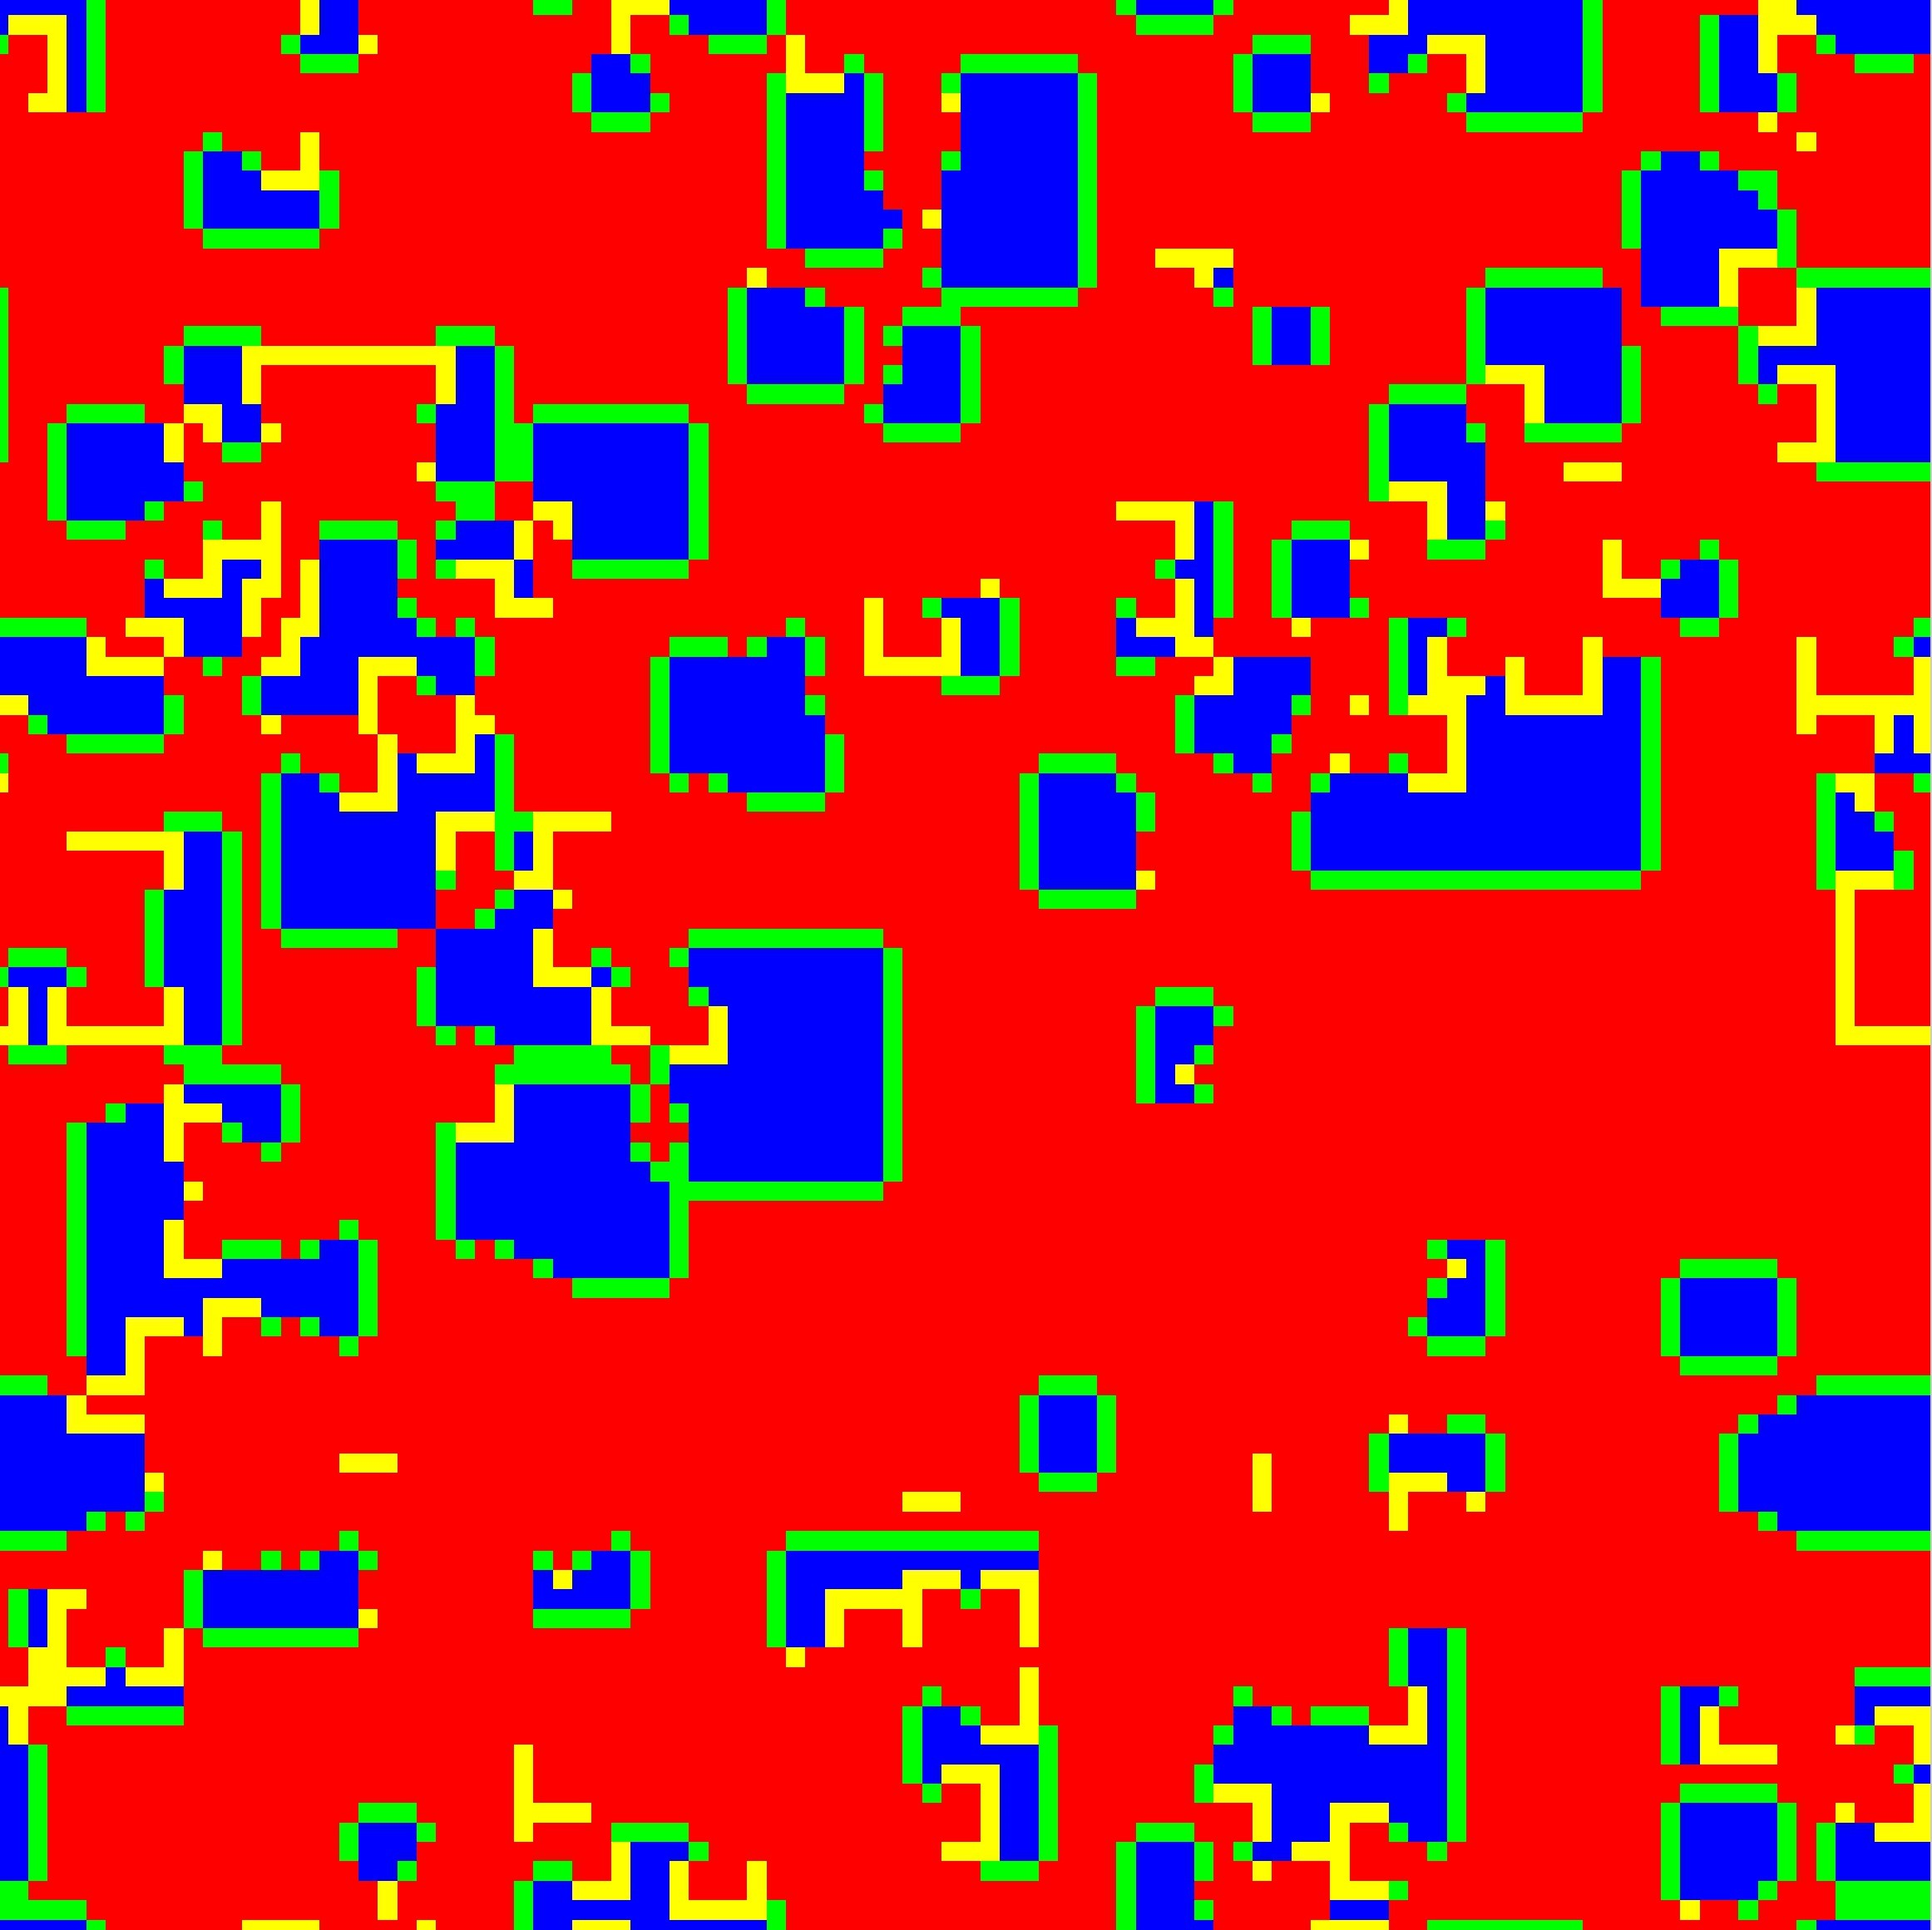
\includegraphics[width=.9\linewidth]{MeanFieldGame/snapshot_b=161.jpg}
          \caption{$b=1.61$}
          \label{fig:sub6}
        \end{subfigure}
        
        \begin{subfigure}{.33\textwidth}
          \centering
          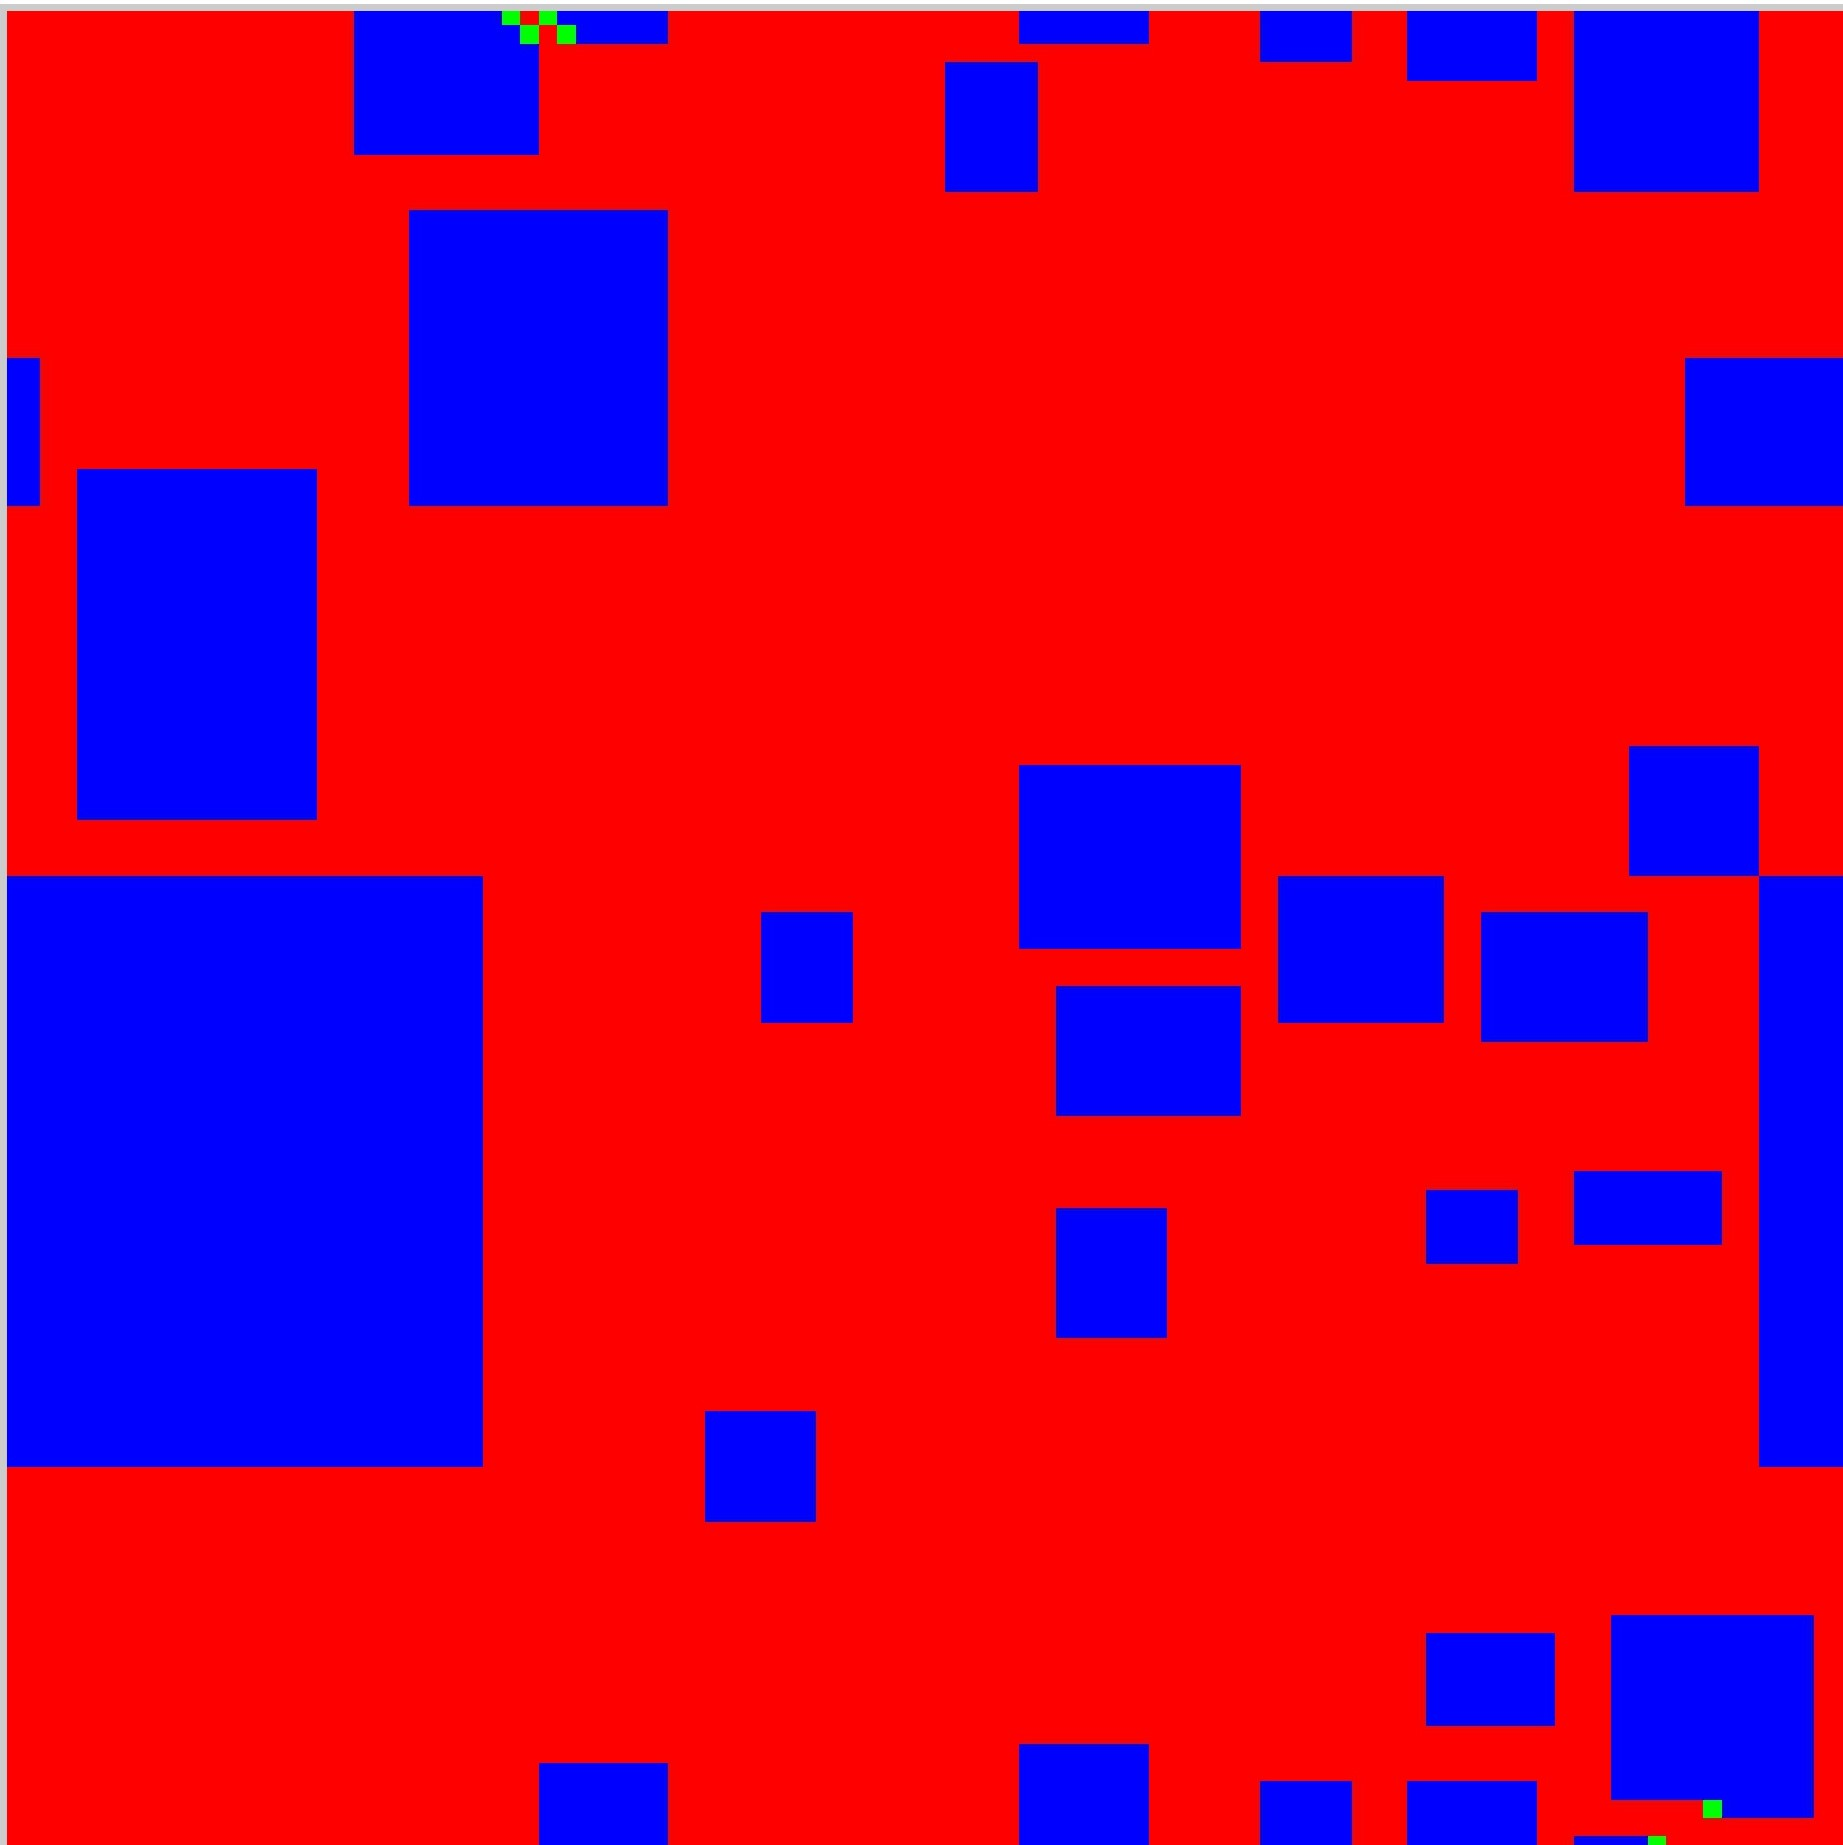
\includegraphics[width=.9\linewidth]{MeanFieldGame/snapshot_b=162.jpg}
          \caption{$b=1.62$}
          \label{fig:sub7}
        \end{subfigure}%
        \begin{subfigure}{.33\textwidth}
          \centering
          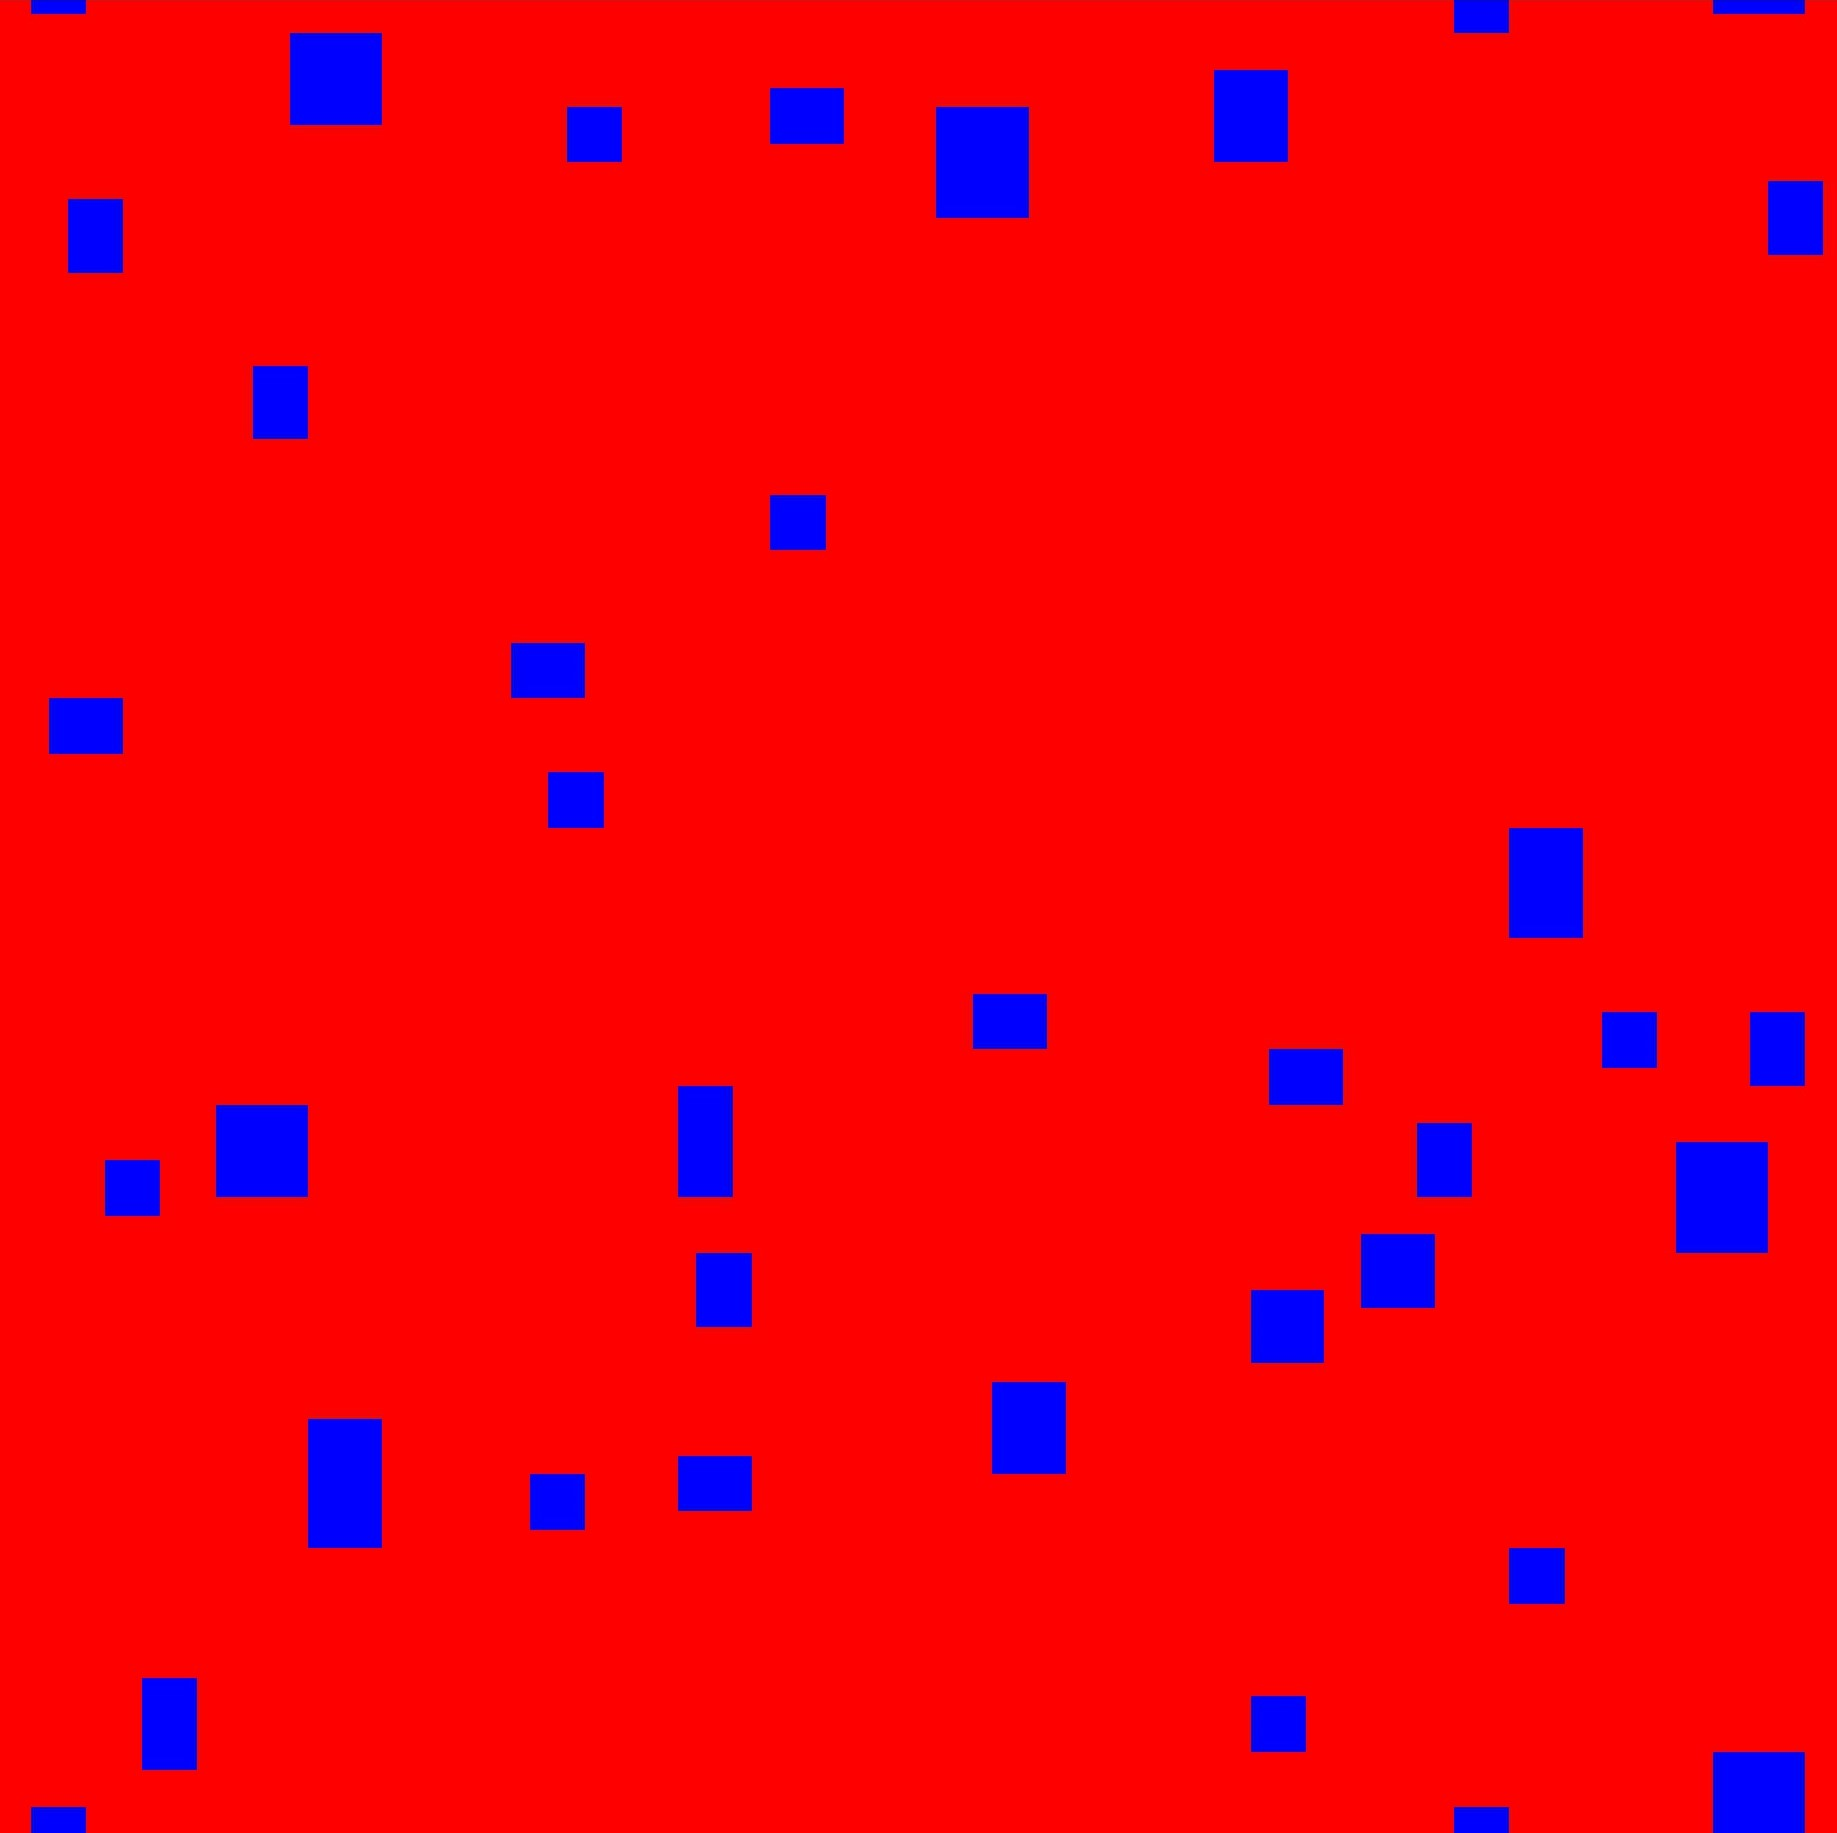
\includegraphics[width=.9\linewidth]{MeanFieldGame/snapshot_b=17.jpg}
          \caption{$b=1.7$}
          \label{fig:sub8}
        \end{subfigure}%
        \begin{subfigure}{.33\textwidth}
          \centering
          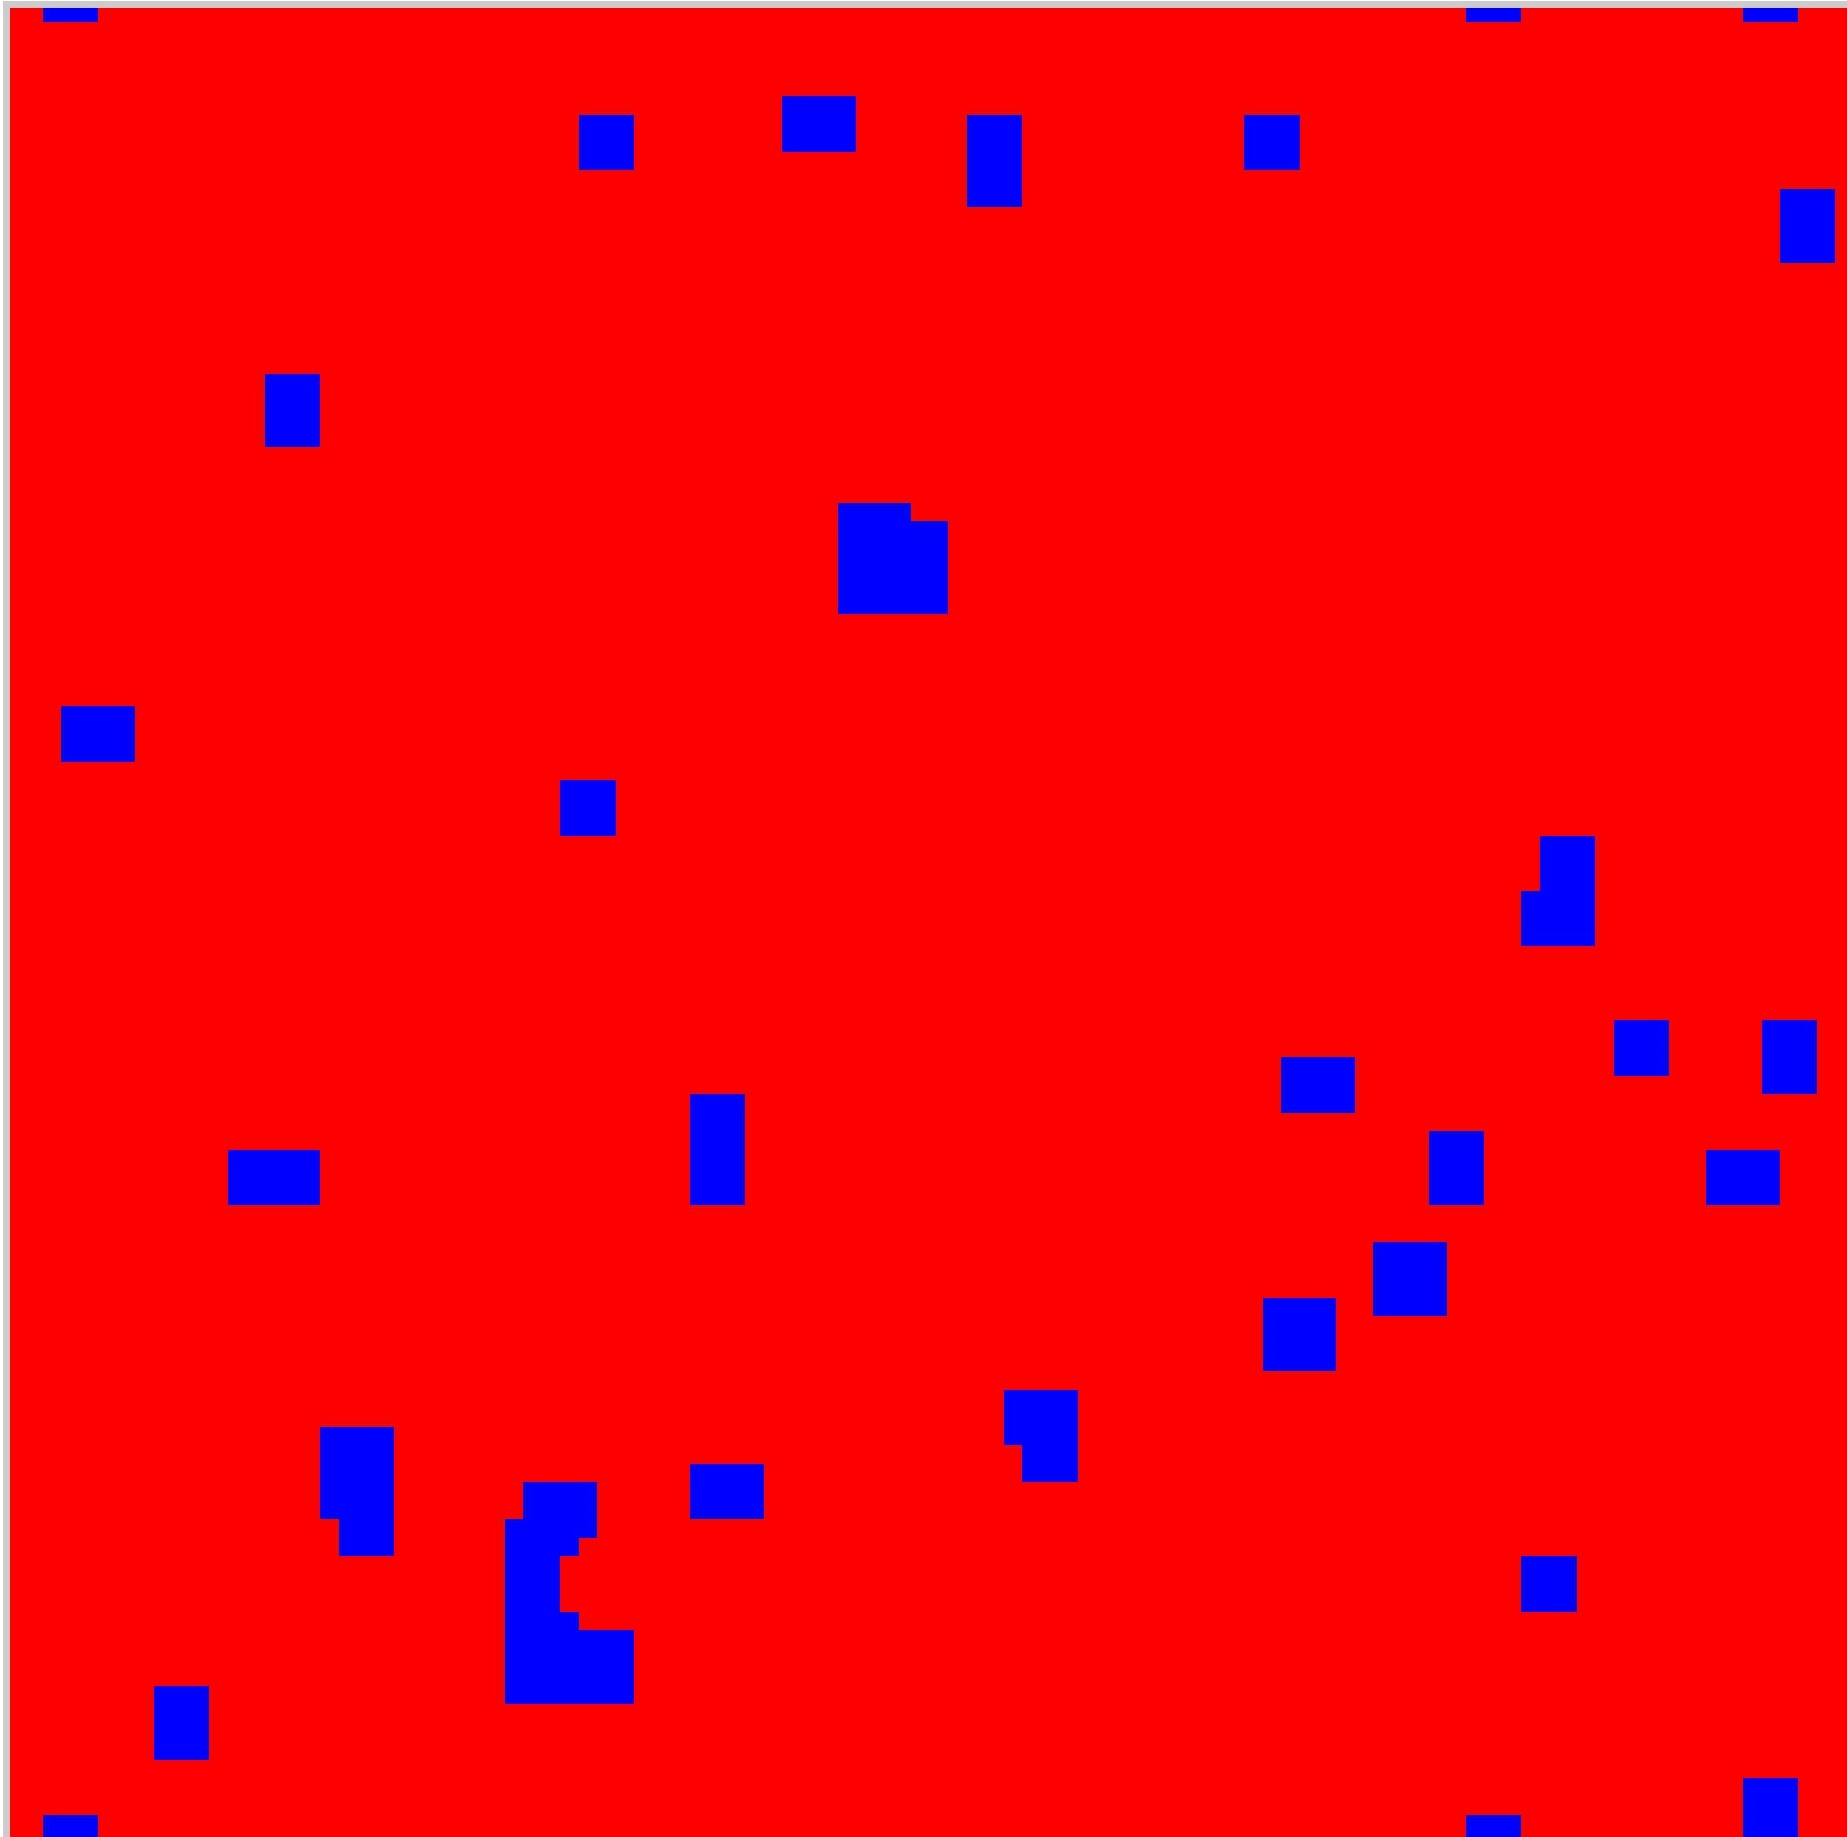
\includegraphics[width=.9\linewidth]{MeanFieldGame/snapshot_b=18.jpg}
          \caption{$b=1.8$}
          \label{fig:sub9}
        \end{subfigure}
    
        
        \caption{ Примеры полей 100 на 100 при начальной плотности $0.9$ после 5000 шагов.\\
        Синий — кооператоры\\
        Красный — дефекторы\\
        Желтый — кооператоры, ставшие дефекторами(на данном ходе)\\
        Зеленый — дефекторы, ставшие кооператорами(на данном ходе)}
        \label{fig:fields}
    \end{figure}
    
\subsection{Распределение числа соседей и размеров кластеров на гиперболе}
    Распределение при различных значениях можно посмотреть в \href{https://github.com/ADmitri42/spatial-evolutionary-game/blob/master/2DMeanGame.ipynb}{ноутбуке}, так как обе анимации выходят слишком тяжелыми.

\subsection{Коротко о квадратной решетке}
    В отличие от игры Новака-Мэя, в игре со "средним полем" плотность может меняться не скачками, а непрерывно и переход между различными режимами игры становиться более плавным.
    
\section{Треугольная решетка}
\subsection{Результаты моделирования}
    На рис. \ref{fig:payoffvsdensityTr} представлена зависимость средней плотности от выигрыша. Как и при игре на квадратном поле, при игре на треугольной решетке существуют значения, при которых плотность кооператоров($\mathbf{f_c}$) зависит непрерывно от выигрыша($\mathbf{b}$)(рис. \ref{fig:payoffvsdensitytrsq} и \ref{fig:payoffvsdensityTr}).
        
    При игре со средним полем на треугольной решетке, как и при игре Новака-Мэя(\cite{KOLOTEV2018}), пропадает режим, в котором все агенты постоянно меняются(рис. \ref{fig:triangfields})(в отличии от игры на квадратной решетке), но, как видно на рис. \ref{fig:payoffvsdensityTr}, плотность кооператоров падает быстрее, чем при игре Новака-Мэя.
        
    \begin{figure}[!h]
        \centering
        \captionsetup{justification=centering}
        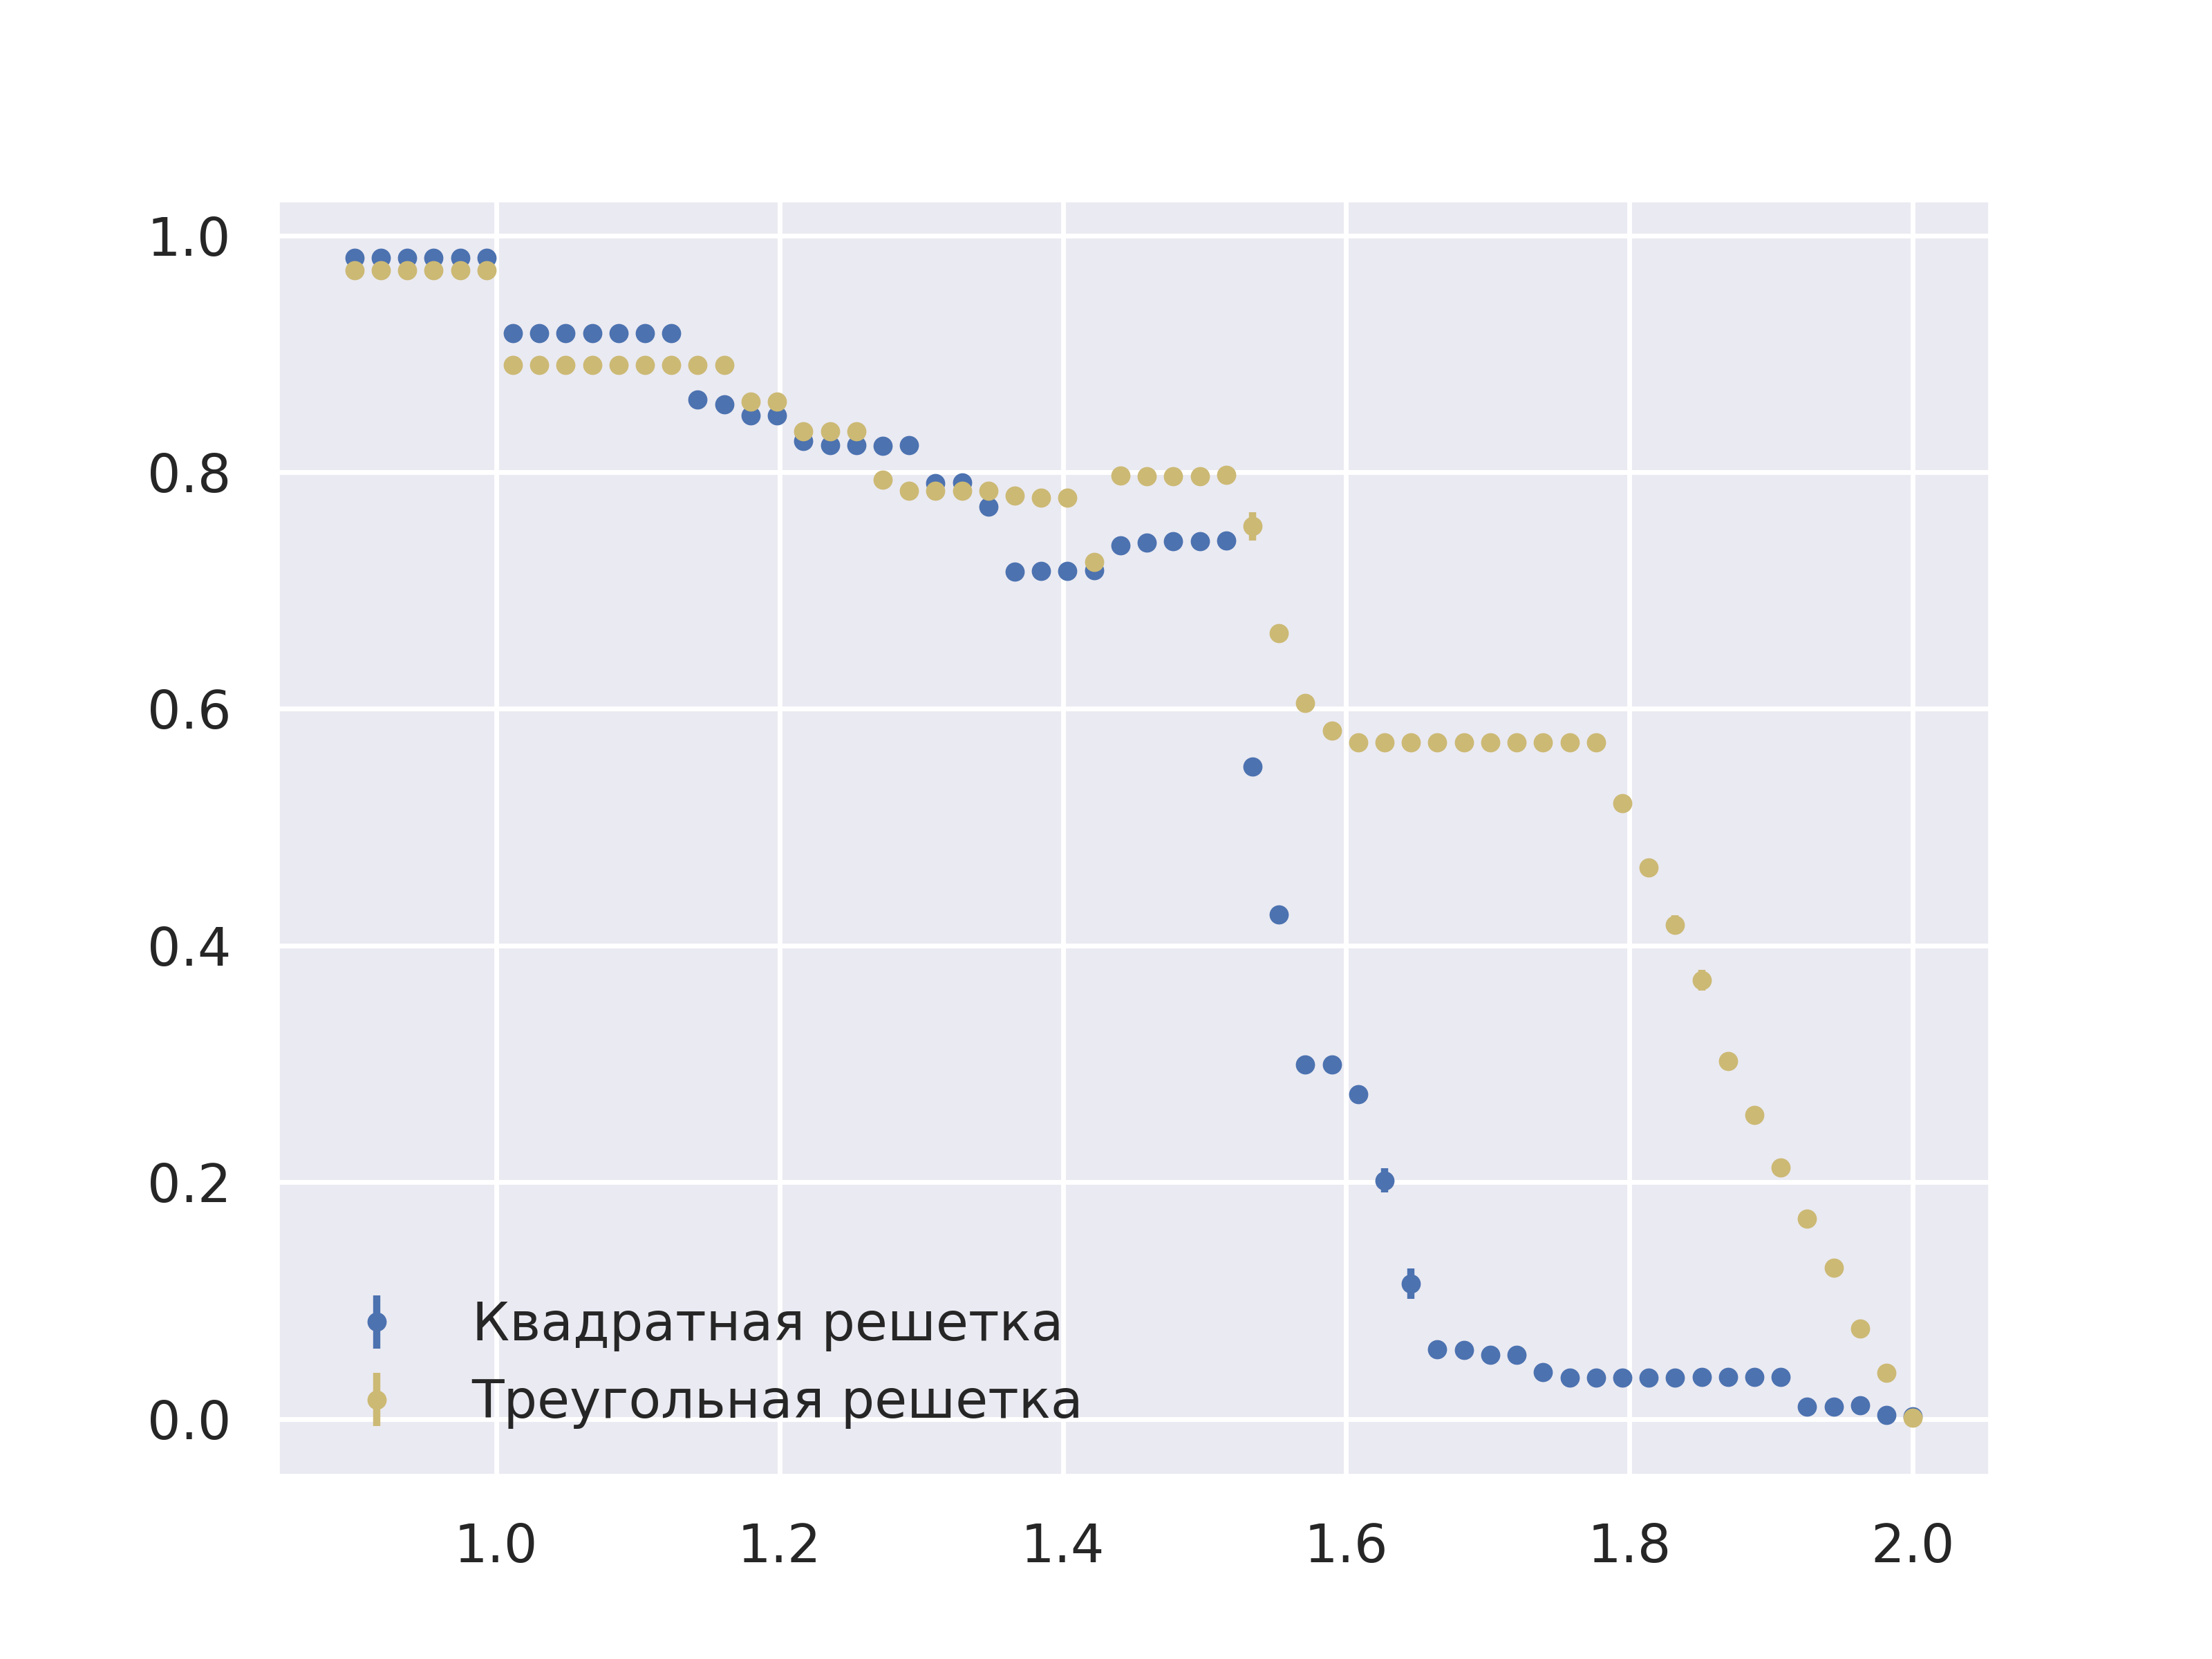
\includegraphics[scale=0.8]{TriangularMeanFieldGame/density_square_triangular.png}
        \caption{Зависимость средней плотности кооператоров от выигрыша на квадратной и треугольной решетке. Погрешности указаны.\\
        Рассчитана на основе 40 случайных реализация начальных условий на поле $200\times200$ с начальной плотностью $0.9$.\\
        Плотность для каждой игры рассчитана как среднее 6000 шагов после отбрасывания 10000 шагов. 
        }
        \label{fig:payoffvsdensitytrsq}
    \end{figure}
    
    \begin{figure}[!h]
        \centering
        \captionsetup{justification=centering}
        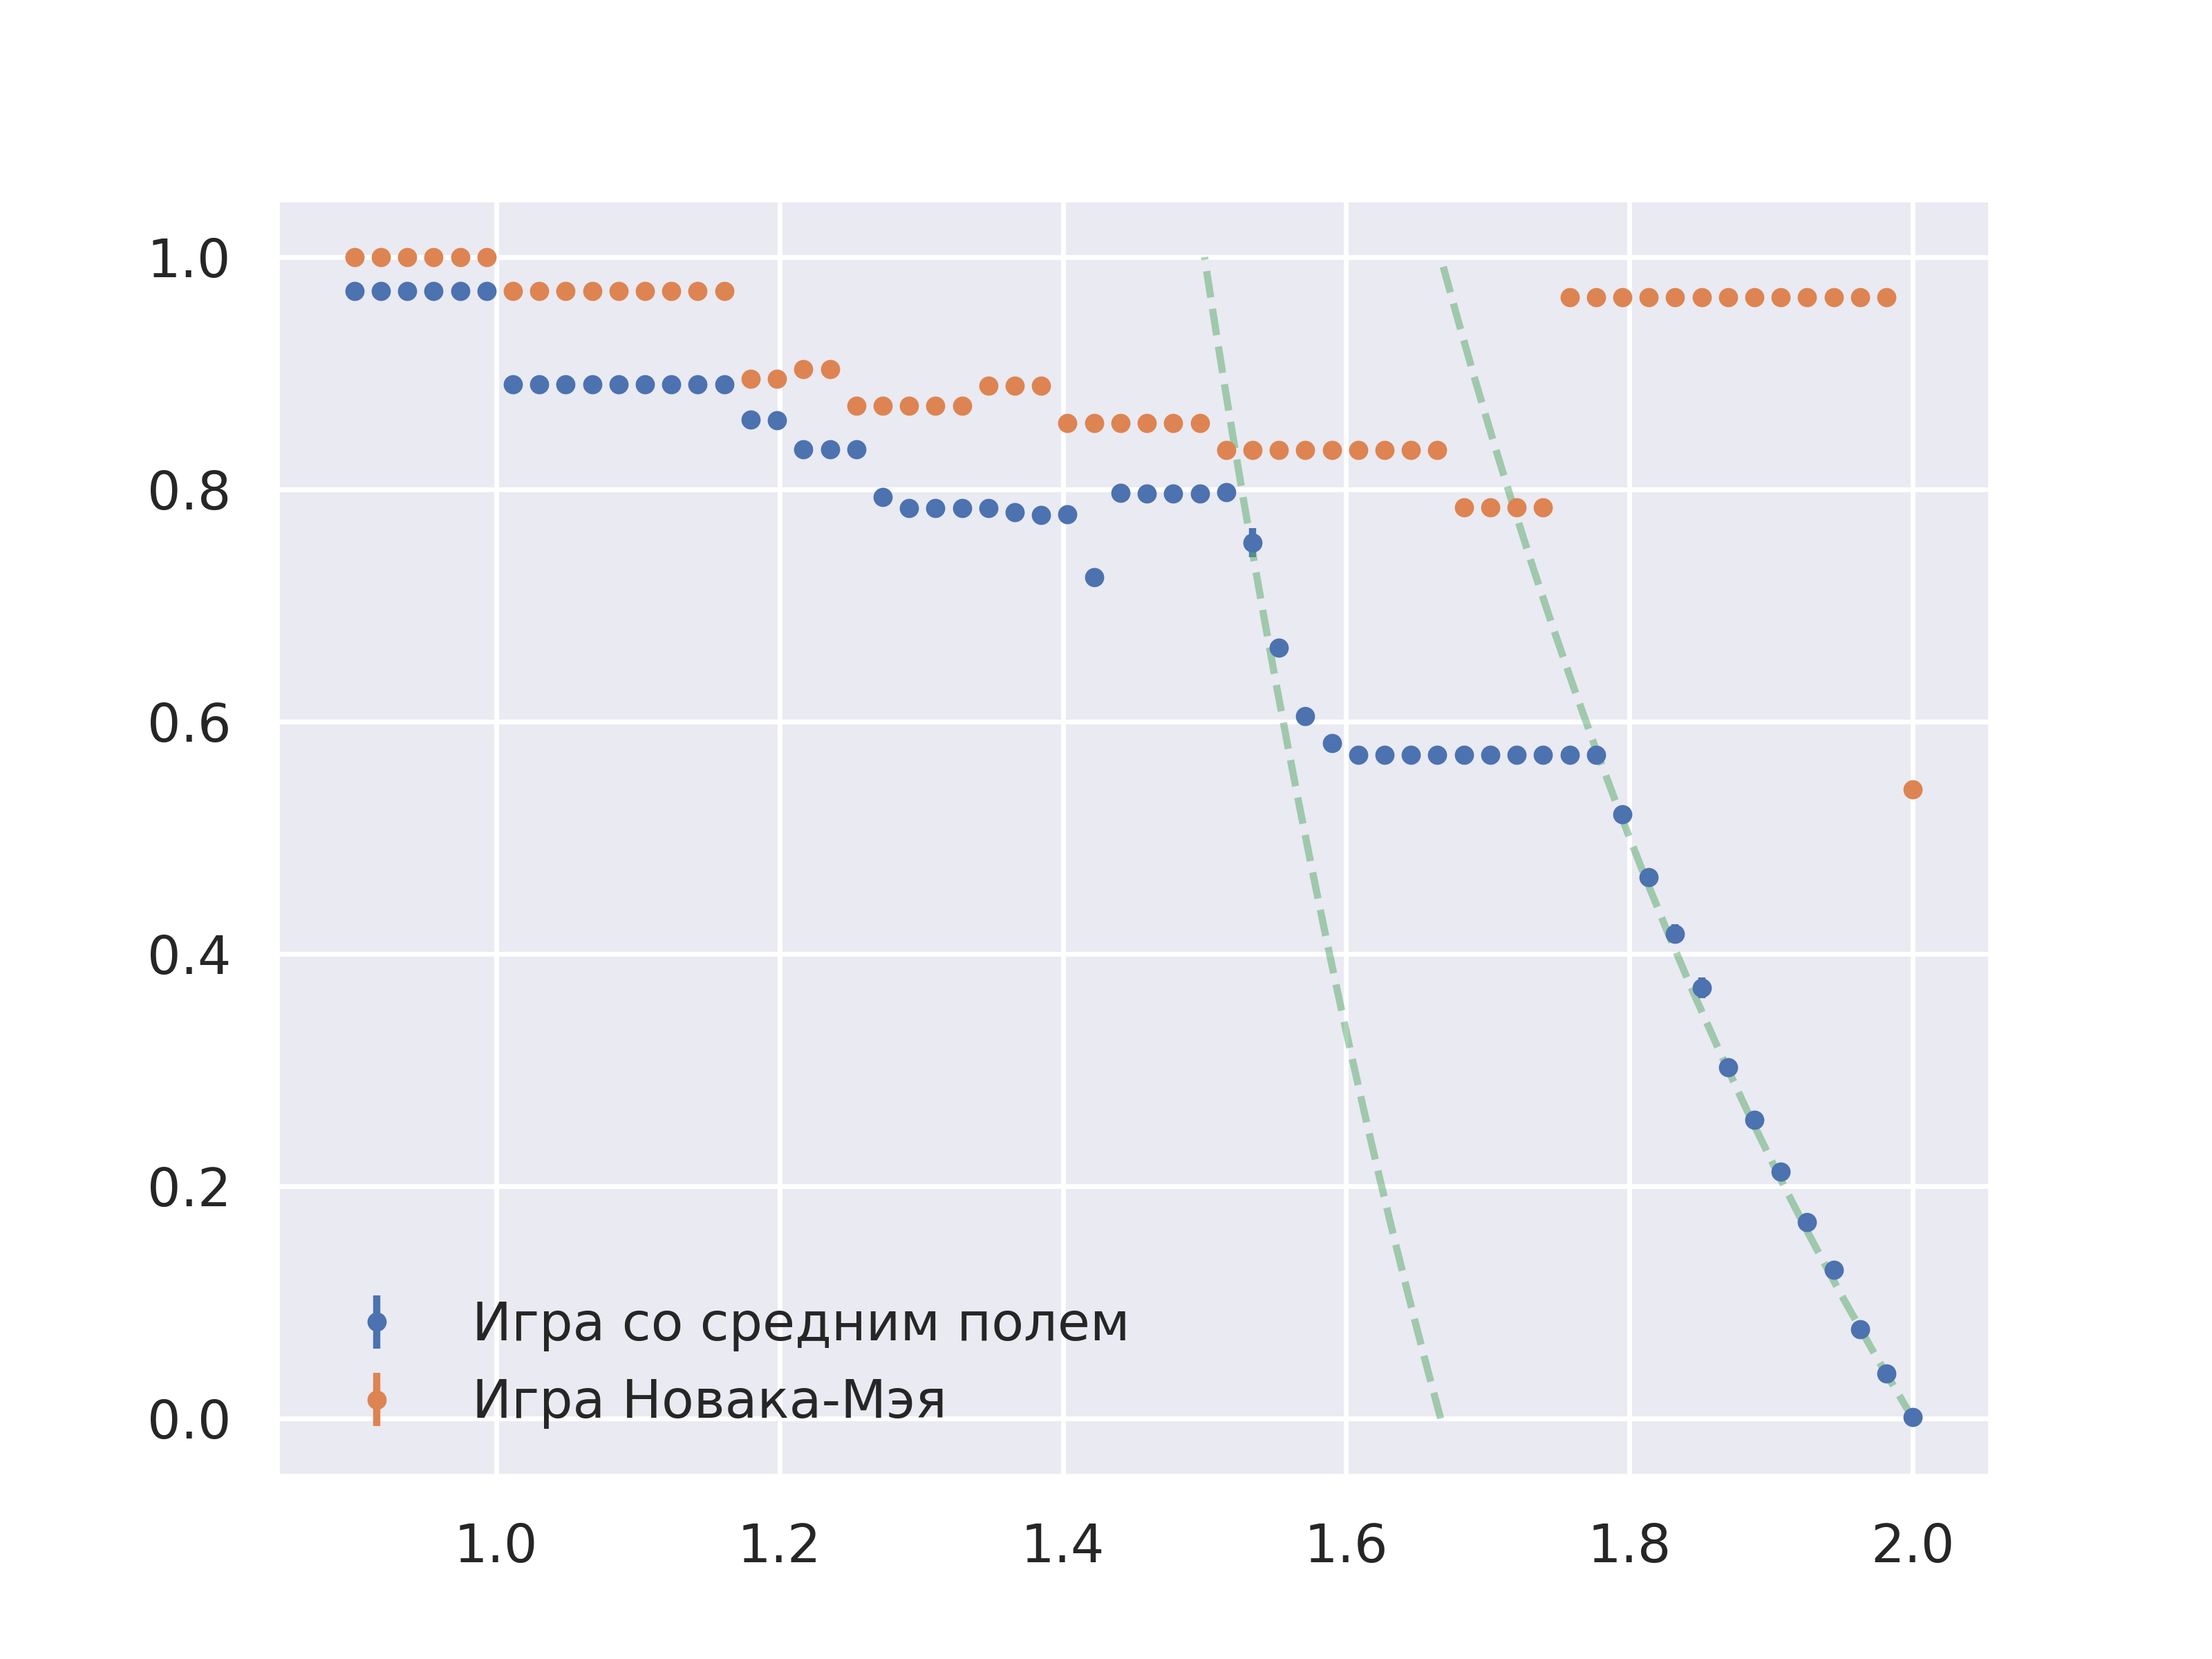
\includegraphics[scale=0.8]{TriangularMeanFieldGame/density_NovakMay_Mean_triangular_game.png}
        \caption{Зависимость средней плотности кооператоров от выигрыша на треугольной решетке и гиперболы $5/3$(левая) и $4/2$(правая). Погрешности указаны.\\
        Рассчитана на основе 40 случайных реализация начальных условий на поле $200\times200$ с начальной плотностью $0.9$.\\
        Плотность для каждой игры рассчитана как среднее 6000 шагов после отбрасывания 10000 шагов. 
        }
        \label{fig:payoffvsdensityTr}
    \end{figure}
    
    
\subsection{Persistence}
    Рассмотрим параметр Persistence - относительное количество игроков, не поменявших стратегию за промежуток $[t_0, t]$
    На рис. \ref{fig:persistencemean} показан Persistence для игры на квадратной и треугольной решетках в зависимости от параметра b. При игре на квадратной решетке существуют значения $b$, при которых в установившемся режиме за 1000 шагов агенты поменяют стратегию($persistence=0$)\footnote{Рассматривается persistence от 15000 до 16000}, но при игре на треугольной решетке $persistence$ не опускается ниже $0.2$ и пропадает хаотический режим.
    
    \begin{figure}[!h]
        \centering
        \captionsetup{justification=centering}
        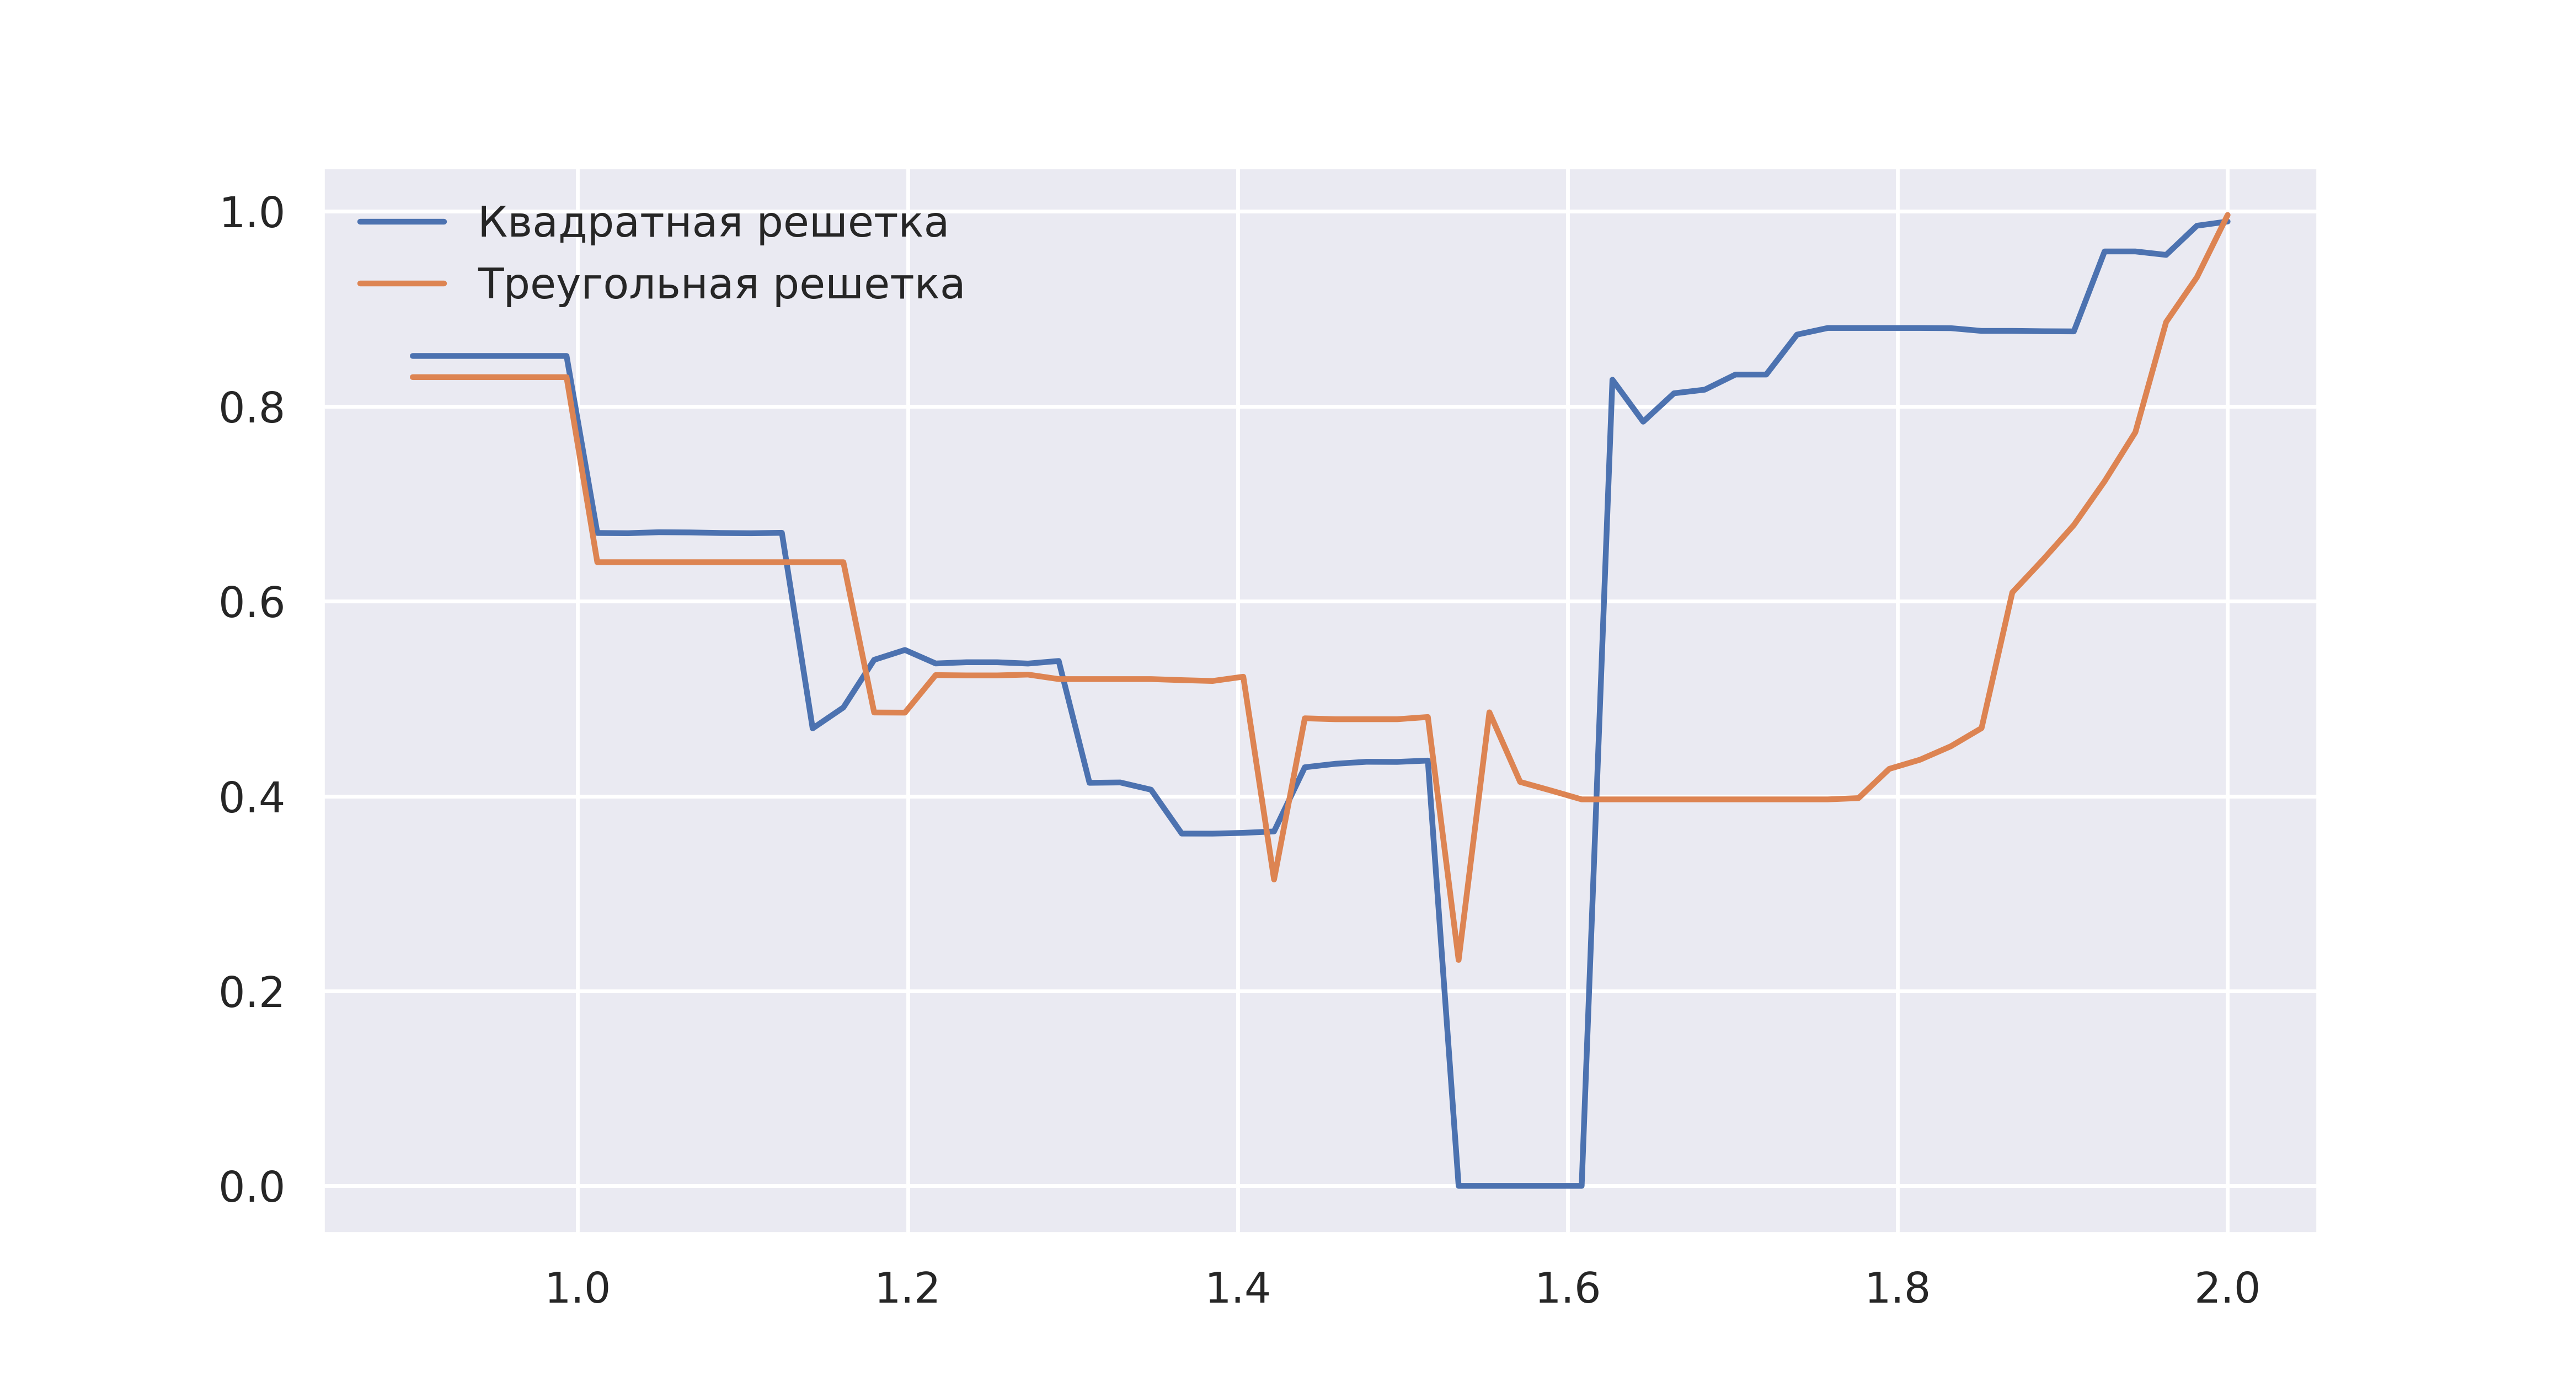
\includegraphics[width=\linewidth]{TriangularMeanFieldGame/persistence.png}
        \caption{Средний persistence на квадратной и треугольной решетке при игре со средним полем\\
        Рассчитан на основе 40 случайных реализация начальных условий на поле $200\times200$ с начальной плотностью $0.9$ от 15000 до 16000.\\
        }
        \label{fig:persistencemean}
    \end{figure}
    
    \begin{figure}[!htbp]
        \centering
        \captionsetup{justification=centering}
        \begin{subfigure}{.33\textwidth}
          \centering
          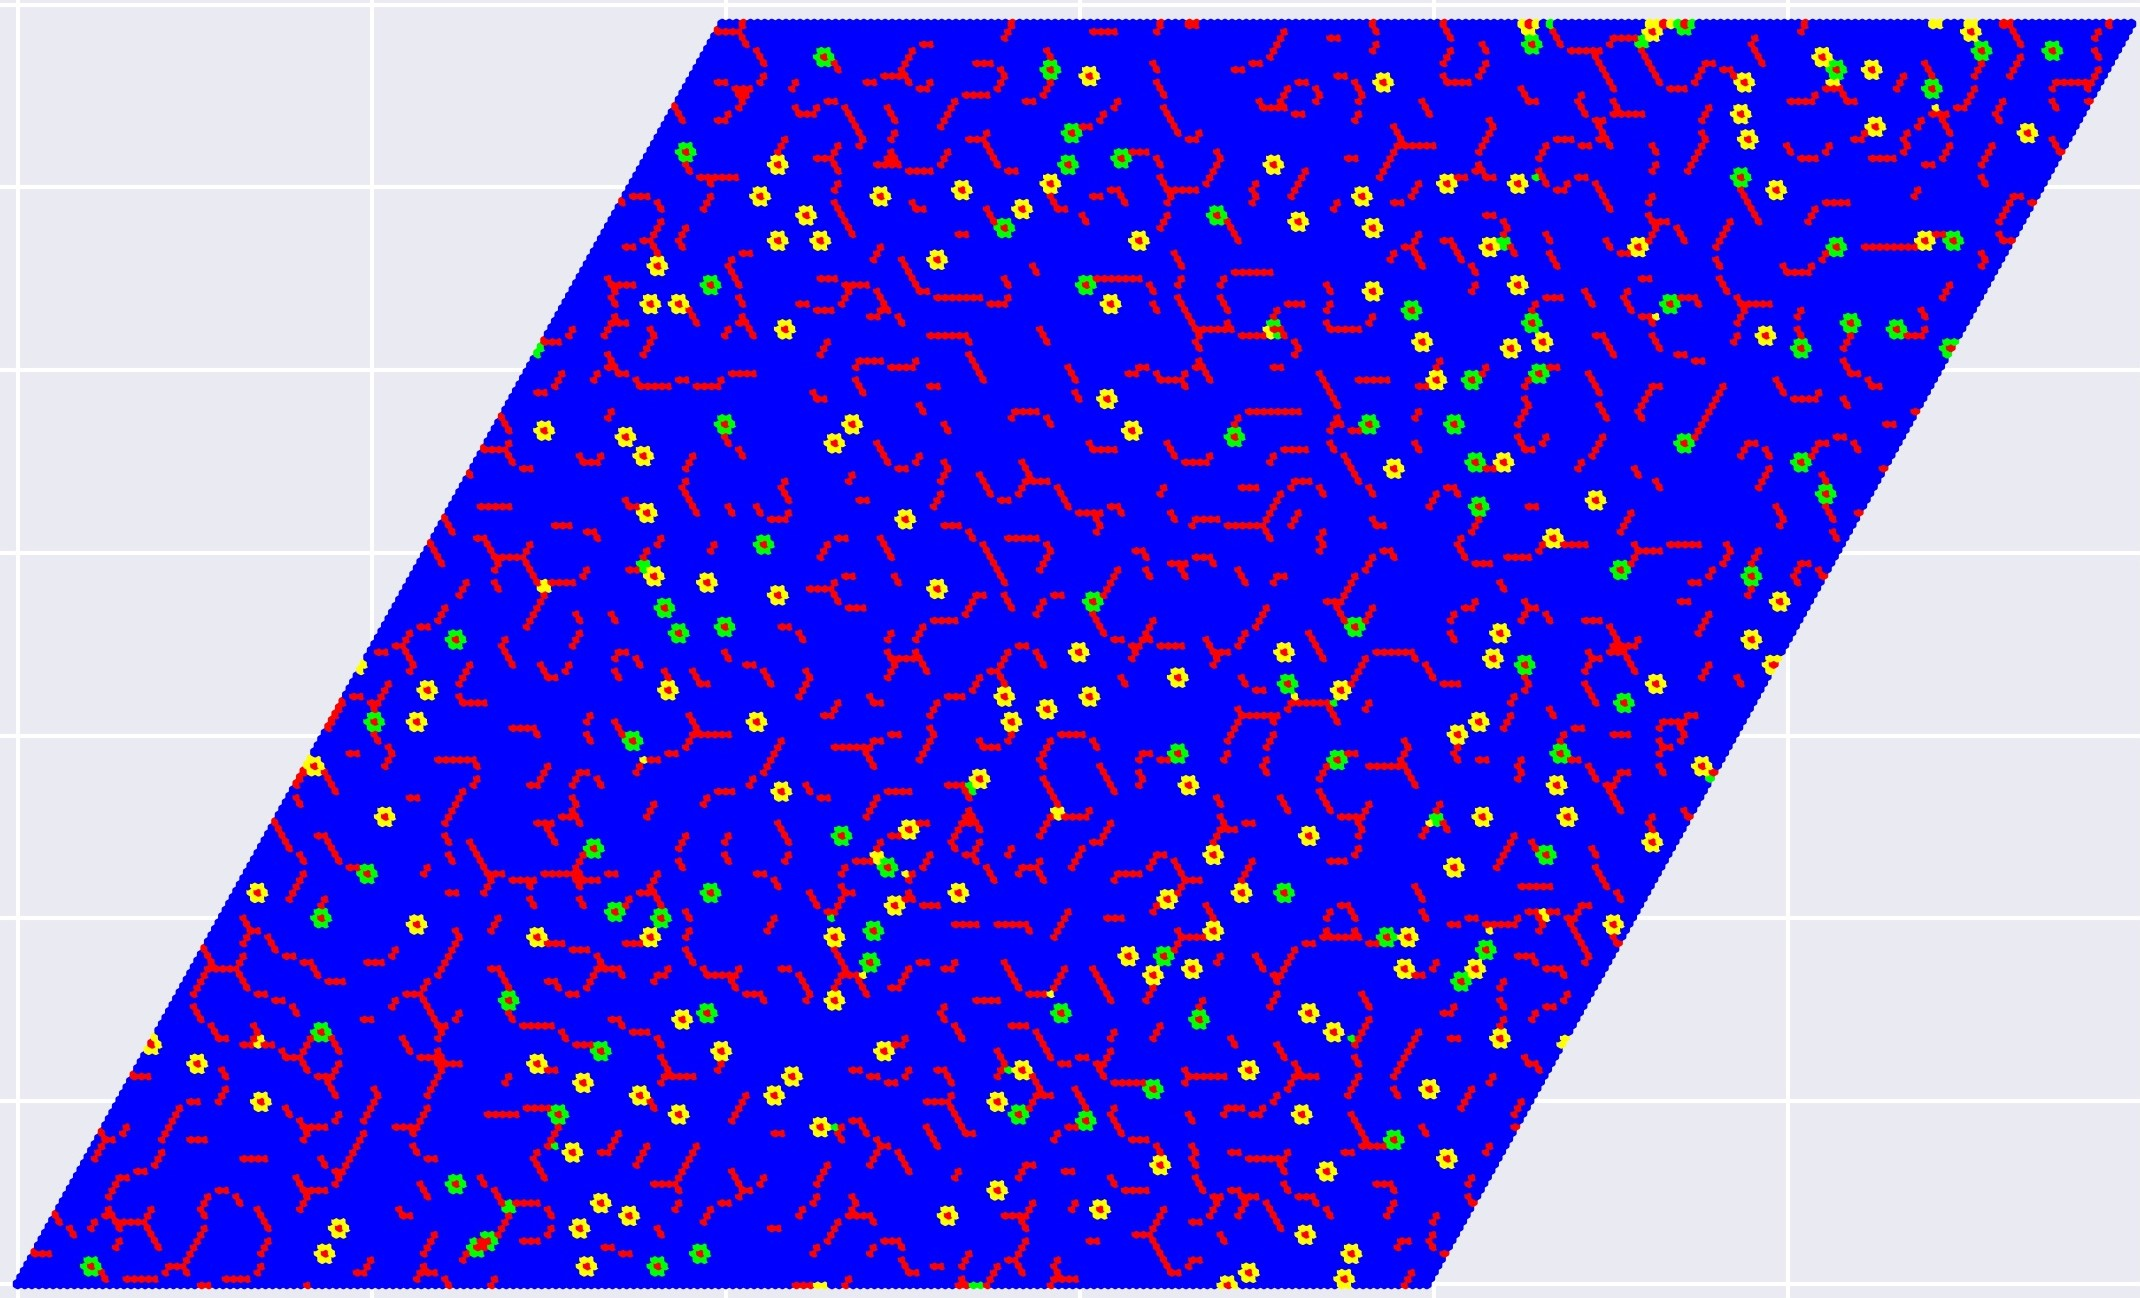
\includegraphics[width=.9\linewidth]{TriangularMeanFieldGame/triangular_snapshot_b=11.jpg}
          \caption{$b=1.1$}
          \label{fig:trsub1}
        \end{subfigure}%
        \begin{subfigure}{.33\textwidth}
          \centering
          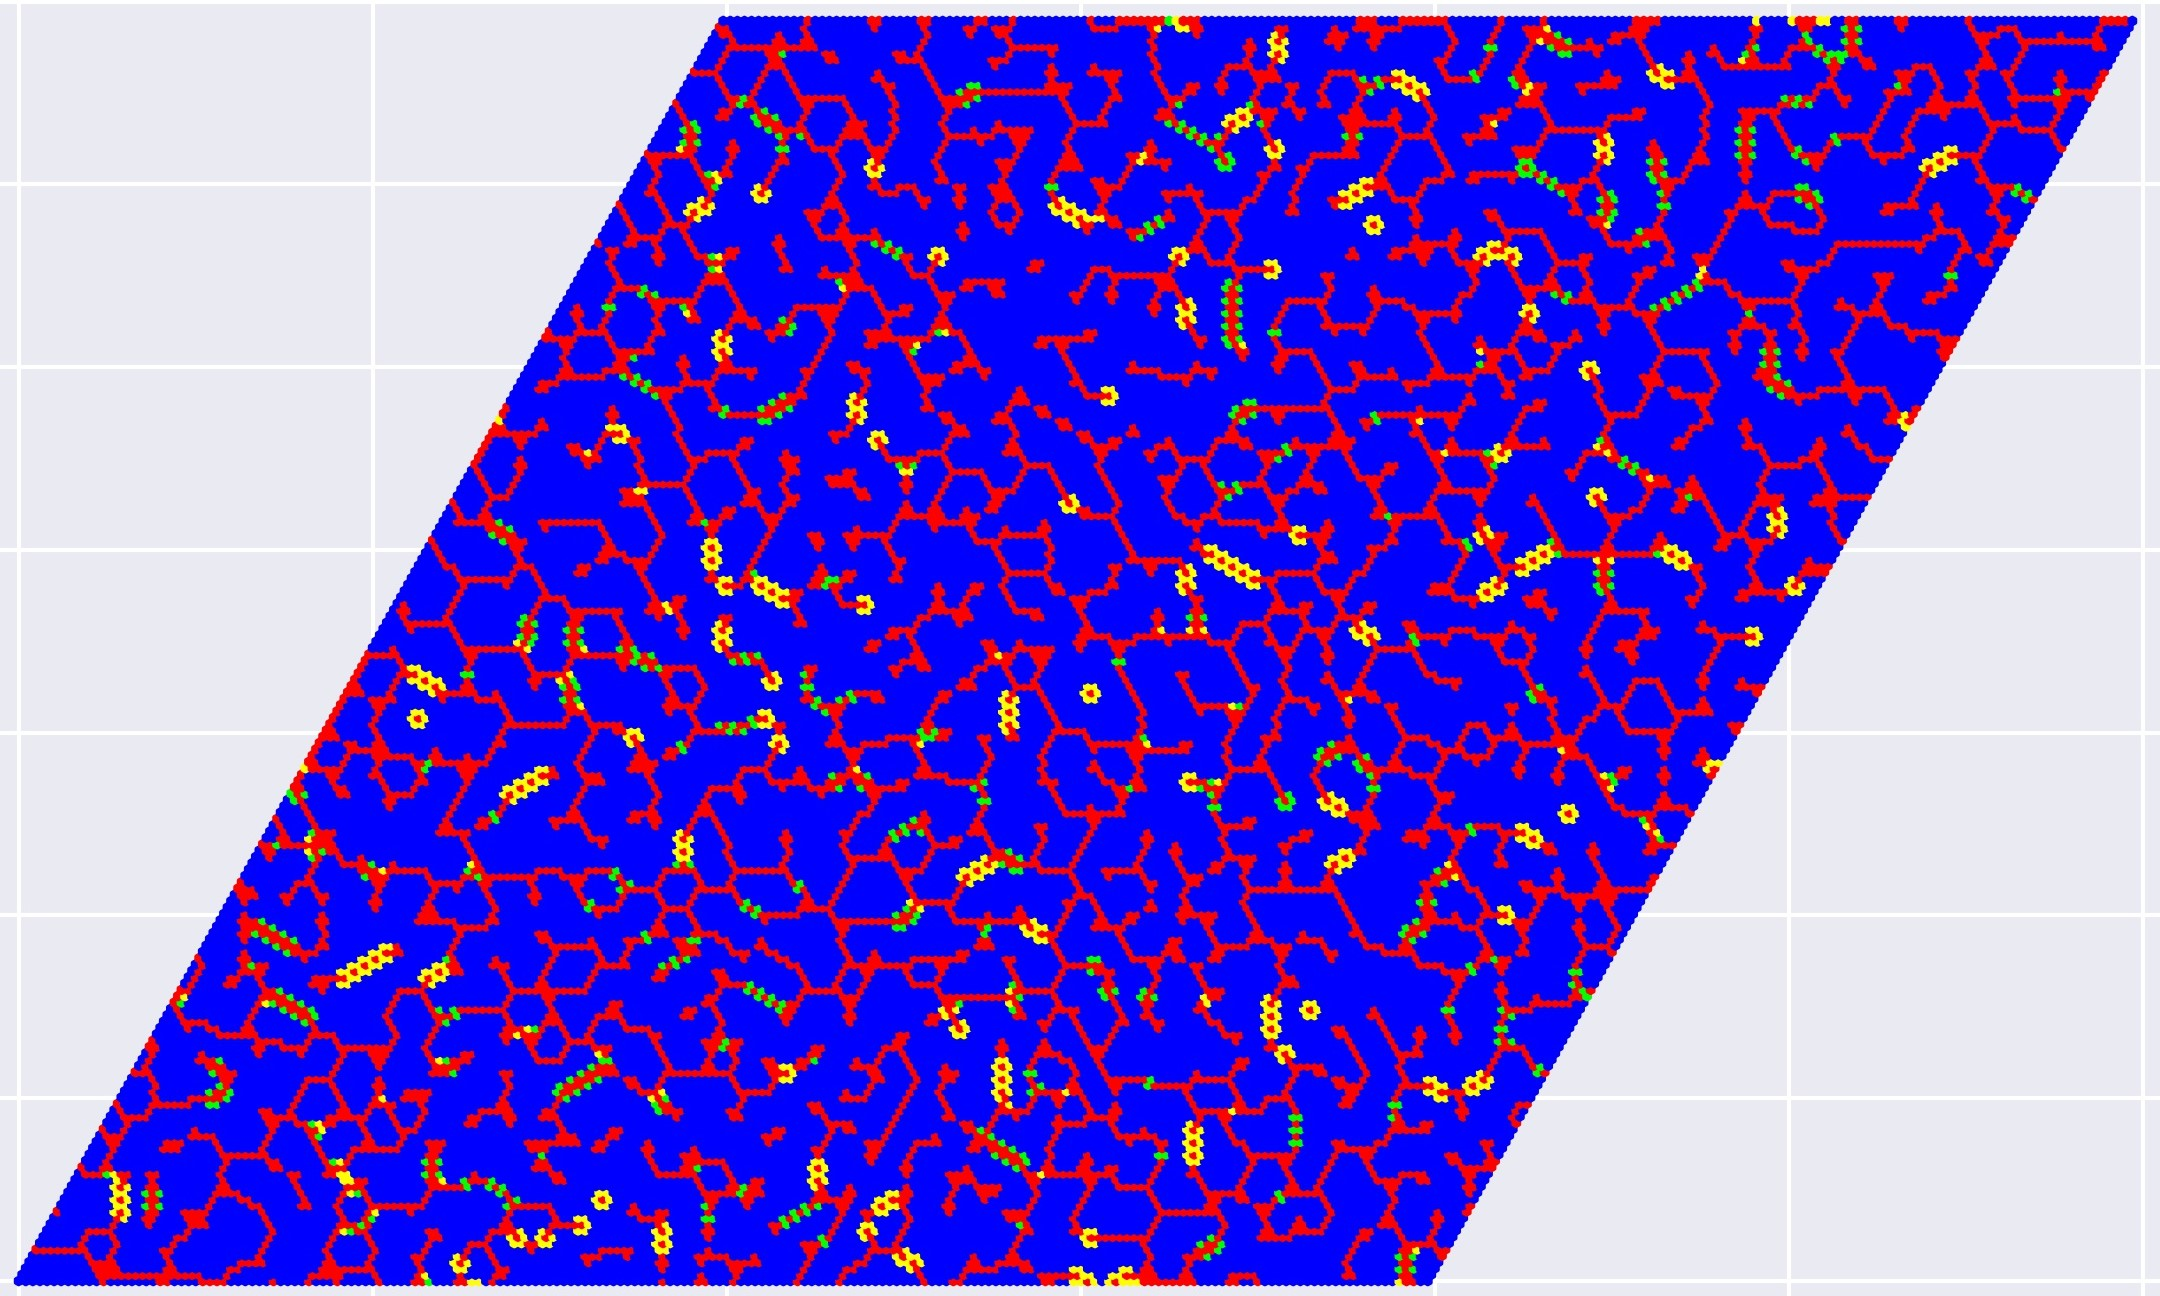
\includegraphics[width=.9\linewidth]{TriangularMeanFieldGame/triangular_snapshot_b=13.jpg}
          \caption{$b=1.3$}
          \label{fig:trsub2}
        \end{subfigure}%
        \begin{subfigure}{.33\textwidth}
          \centering
          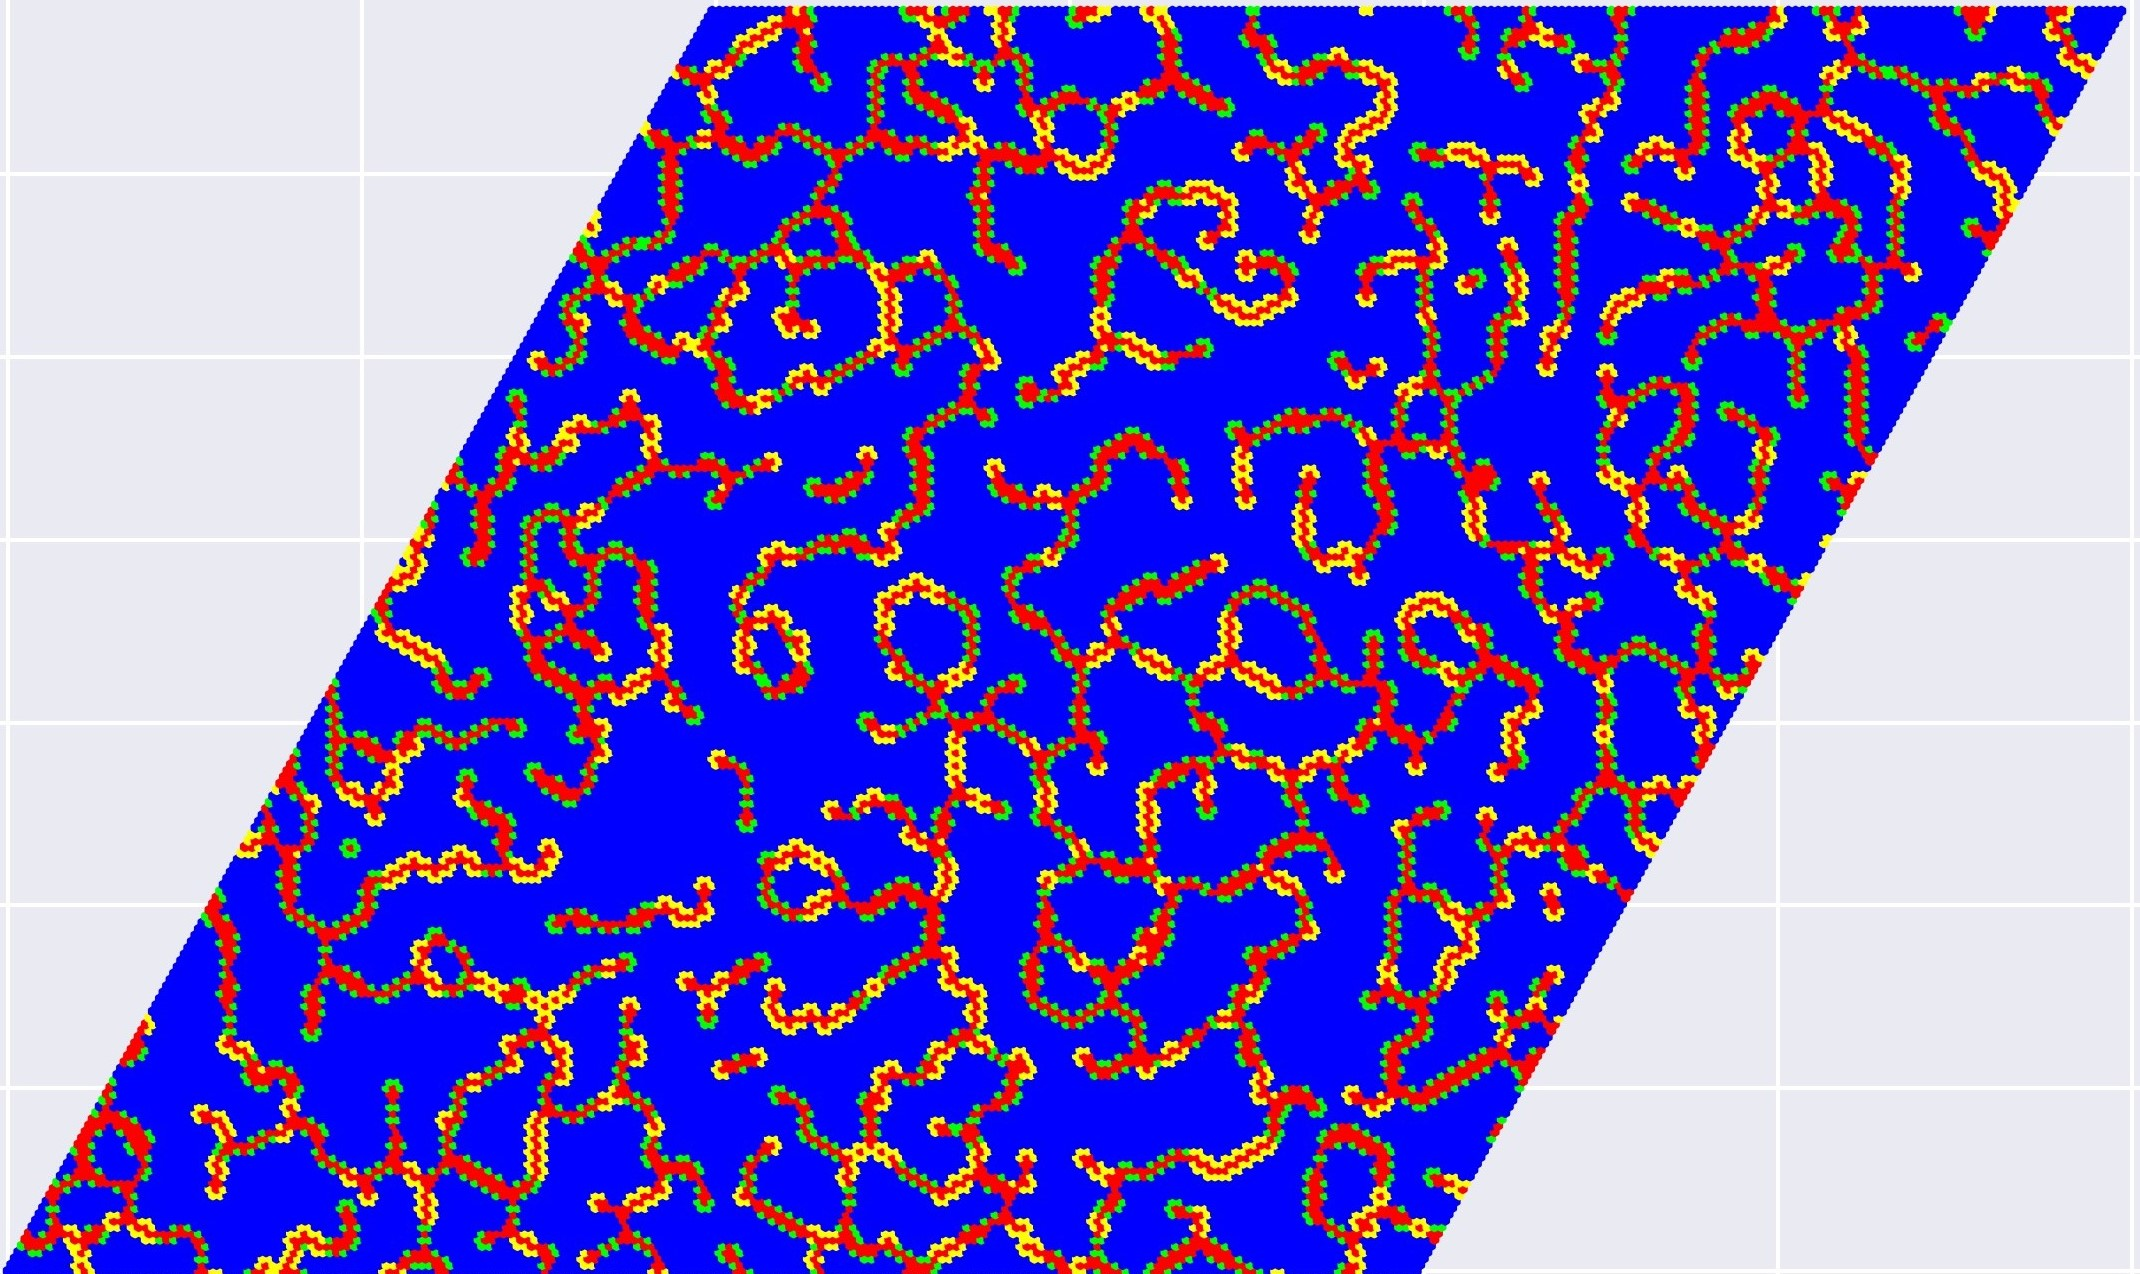
\includegraphics[width=.9\linewidth]{TriangularMeanFieldGame/triangular_snapshot_b=15.jpg}
          \caption{$b=1.5$}
          \label{fig:trsub3}
        \end{subfigure}
        
        \begin{subfigure}{.33\textwidth}
          \centering
          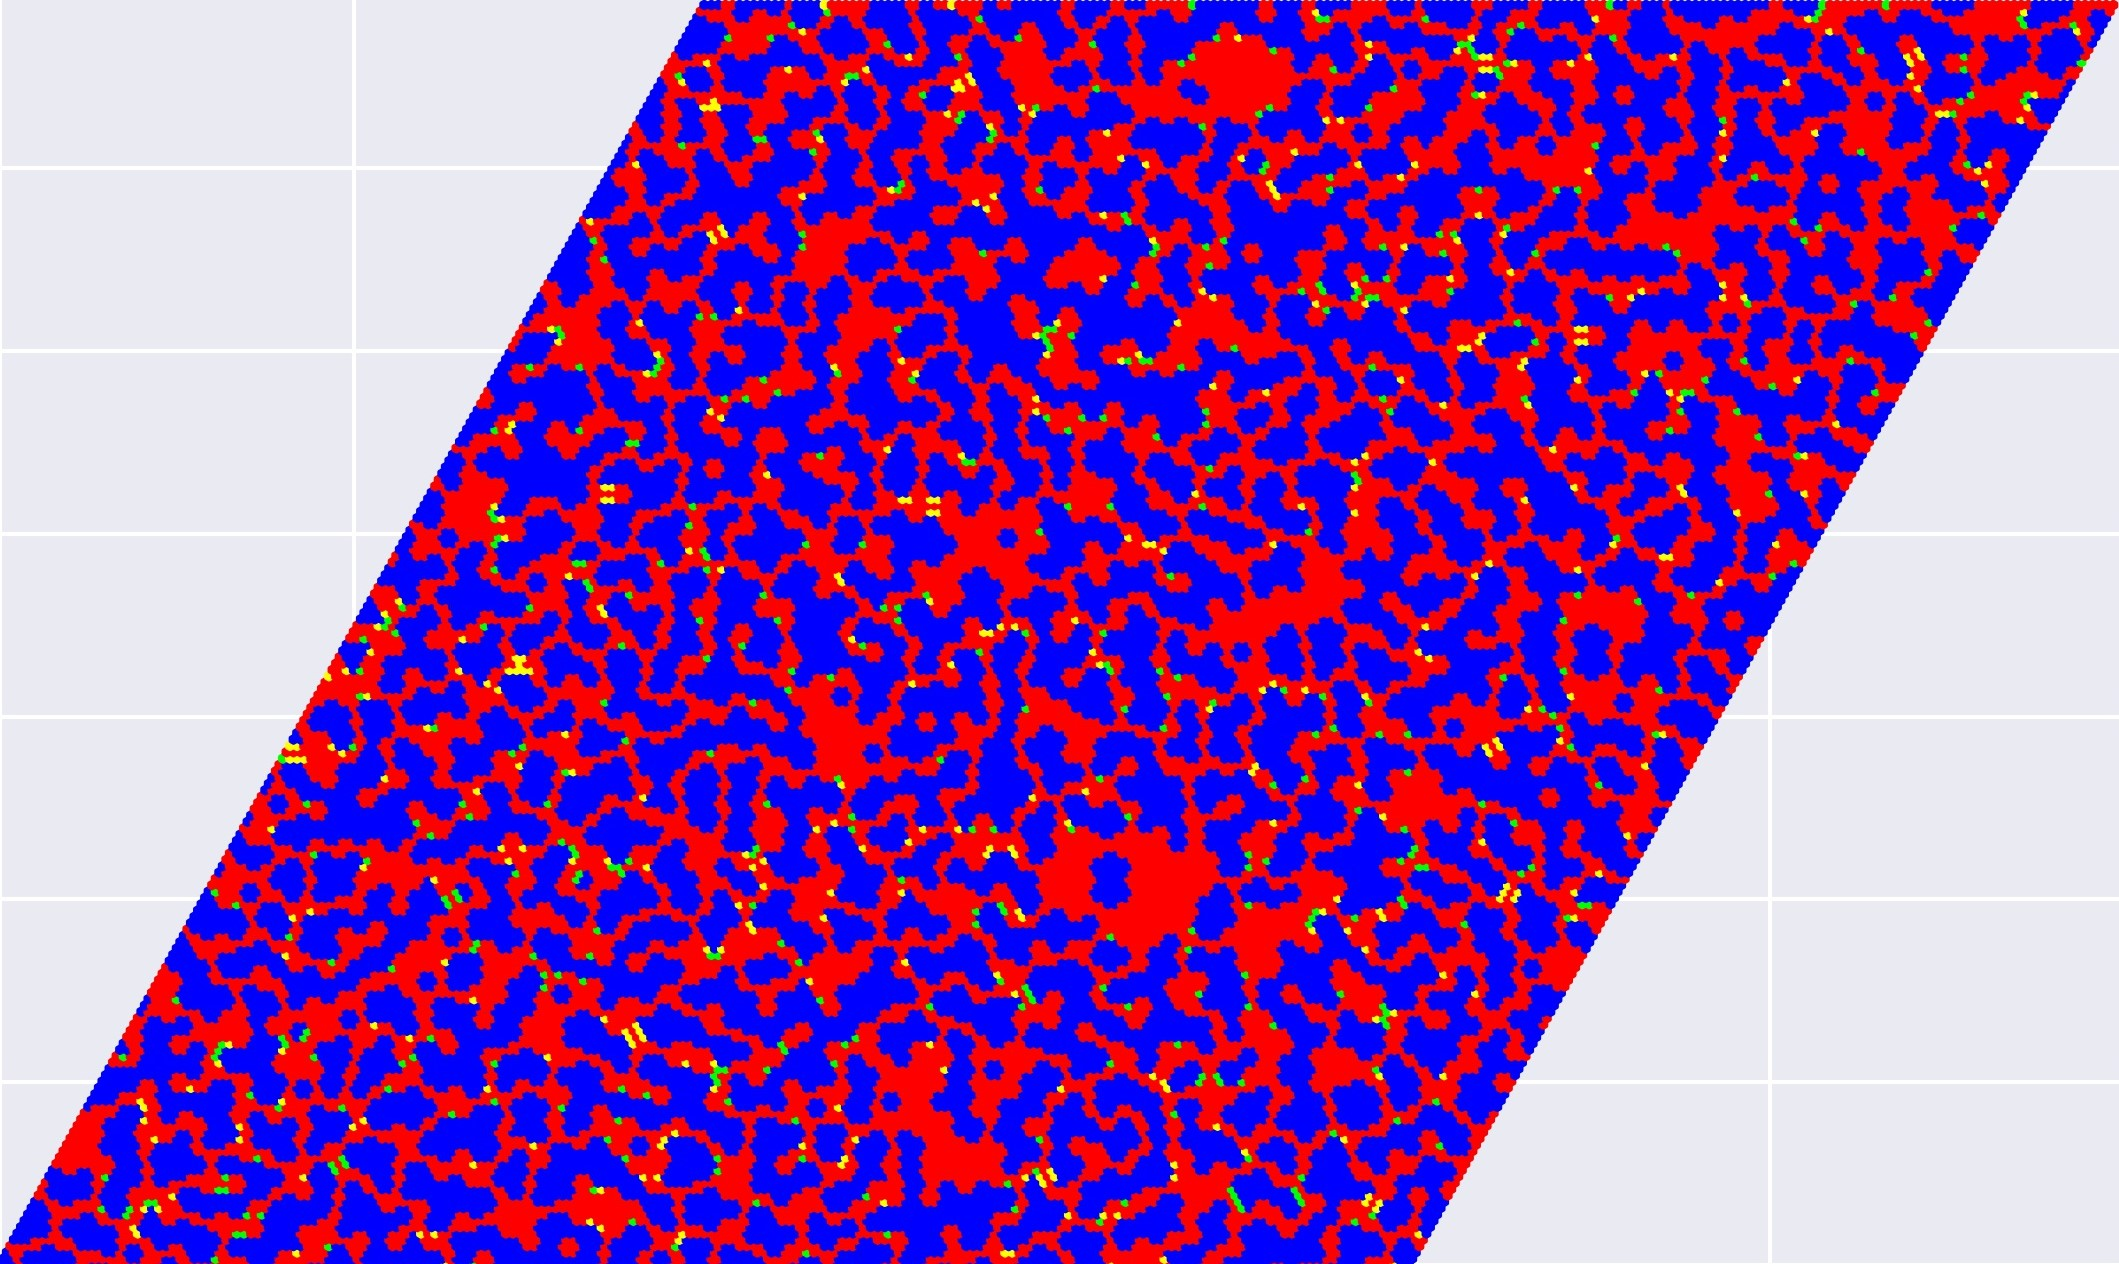
\includegraphics[width=.9\linewidth]{TriangularMeanFieldGame/triangular_snapshot_b=16.jpg}
          \caption{$b=1.6$}
          \label{fig:trsub4}
        \end{subfigure}%
        \begin{subfigure}{.33\textwidth}
          \centering
          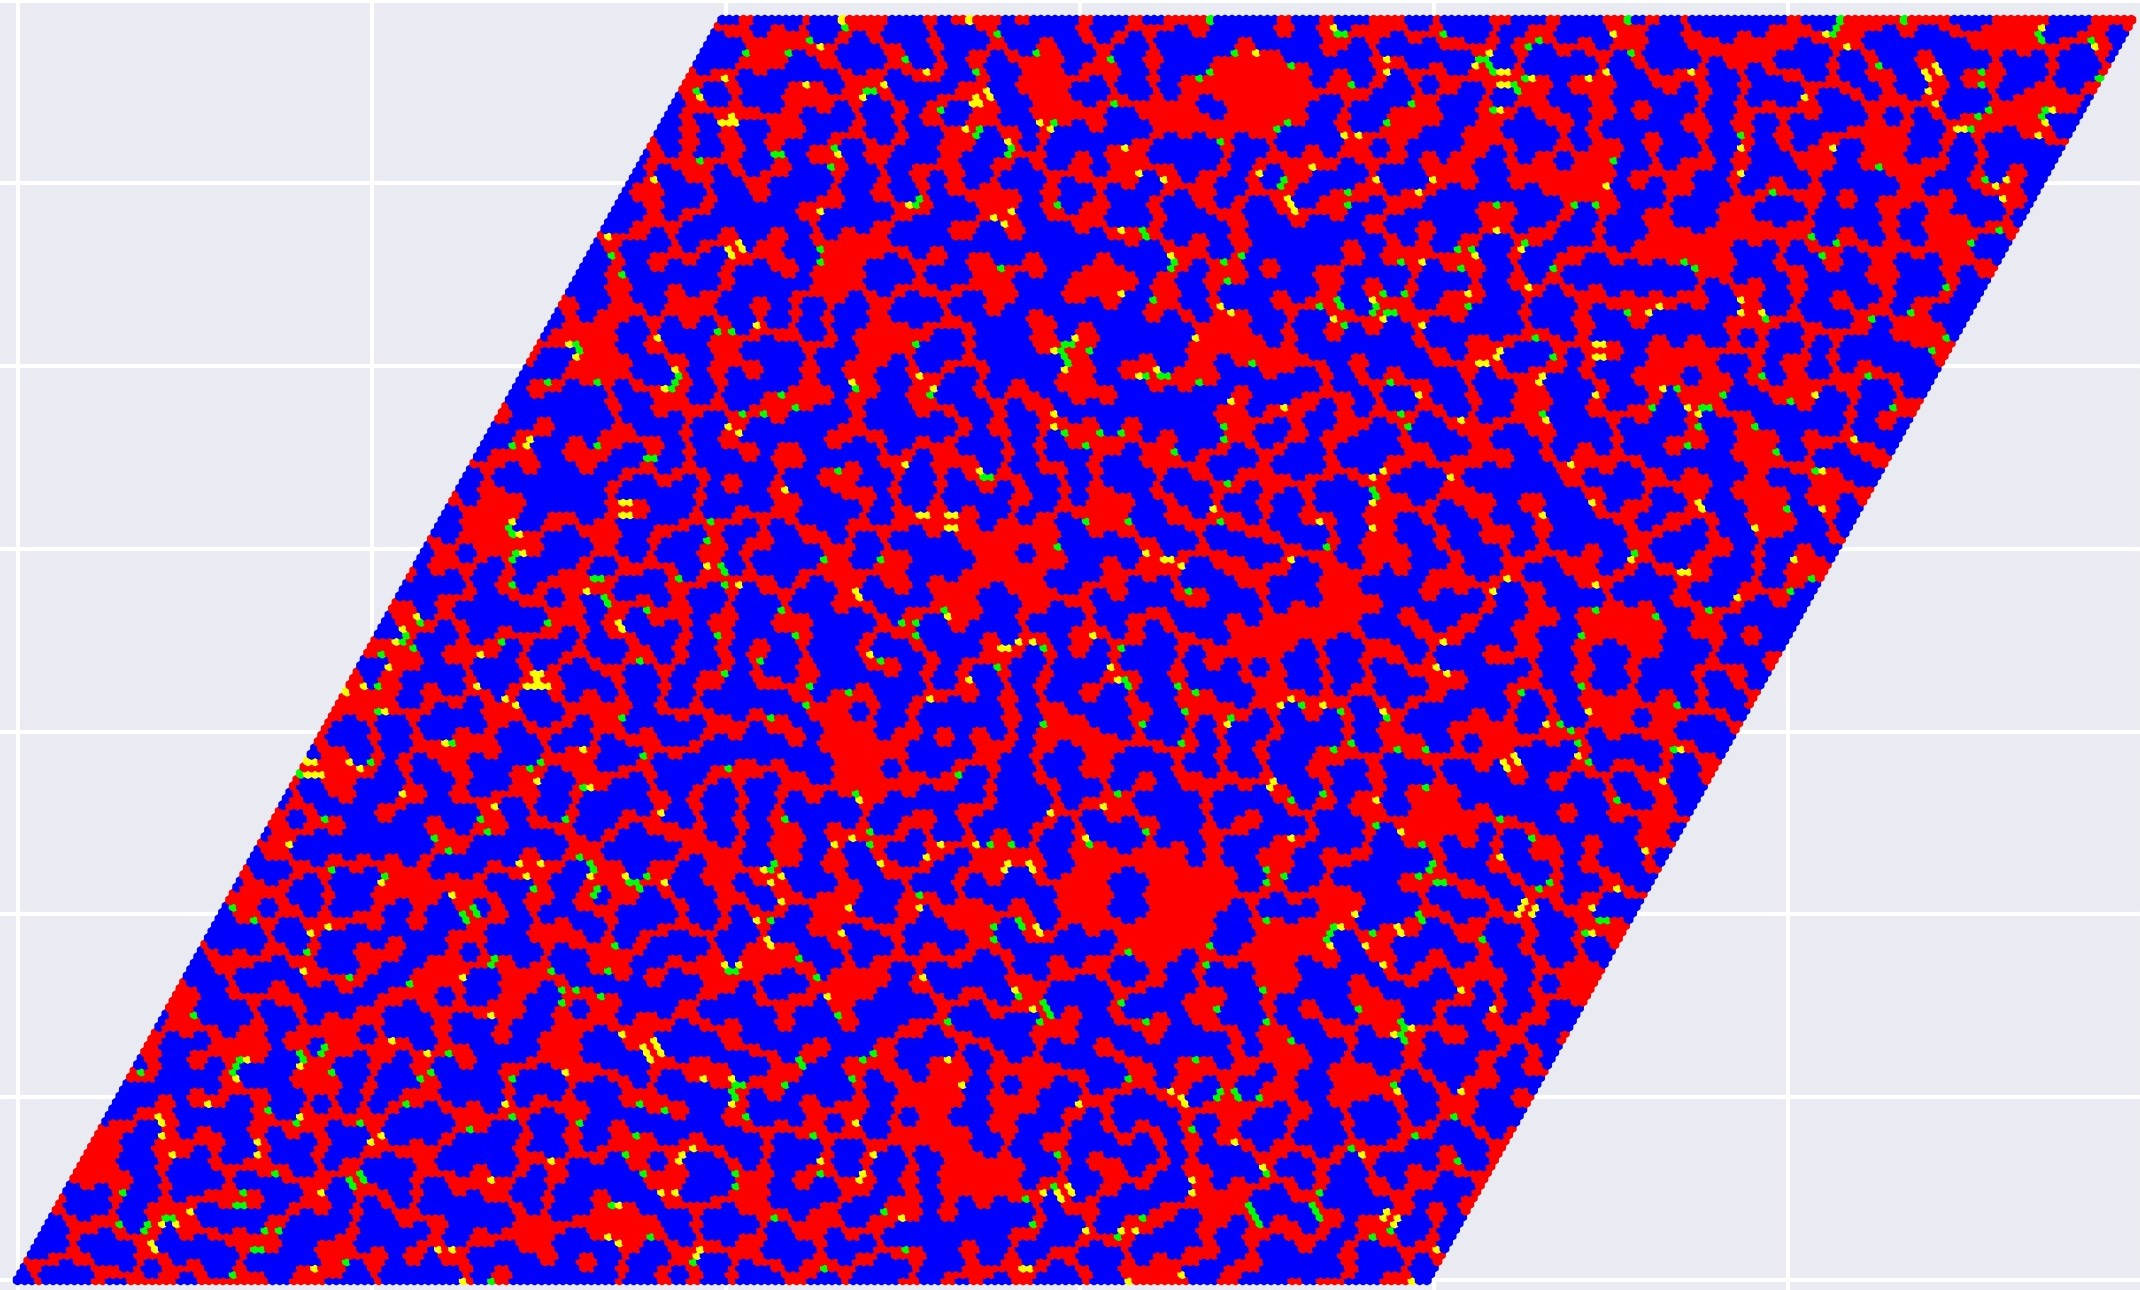
\includegraphics[width=.9\linewidth]{TriangularMeanFieldGame/triangular_snapshot_b=165.jpg}
          \caption{$b=1.65$}
          \label{fig:trsub5}
        \end{subfigure}%
        \begin{subfigure}{.33\textwidth}
          \centering
          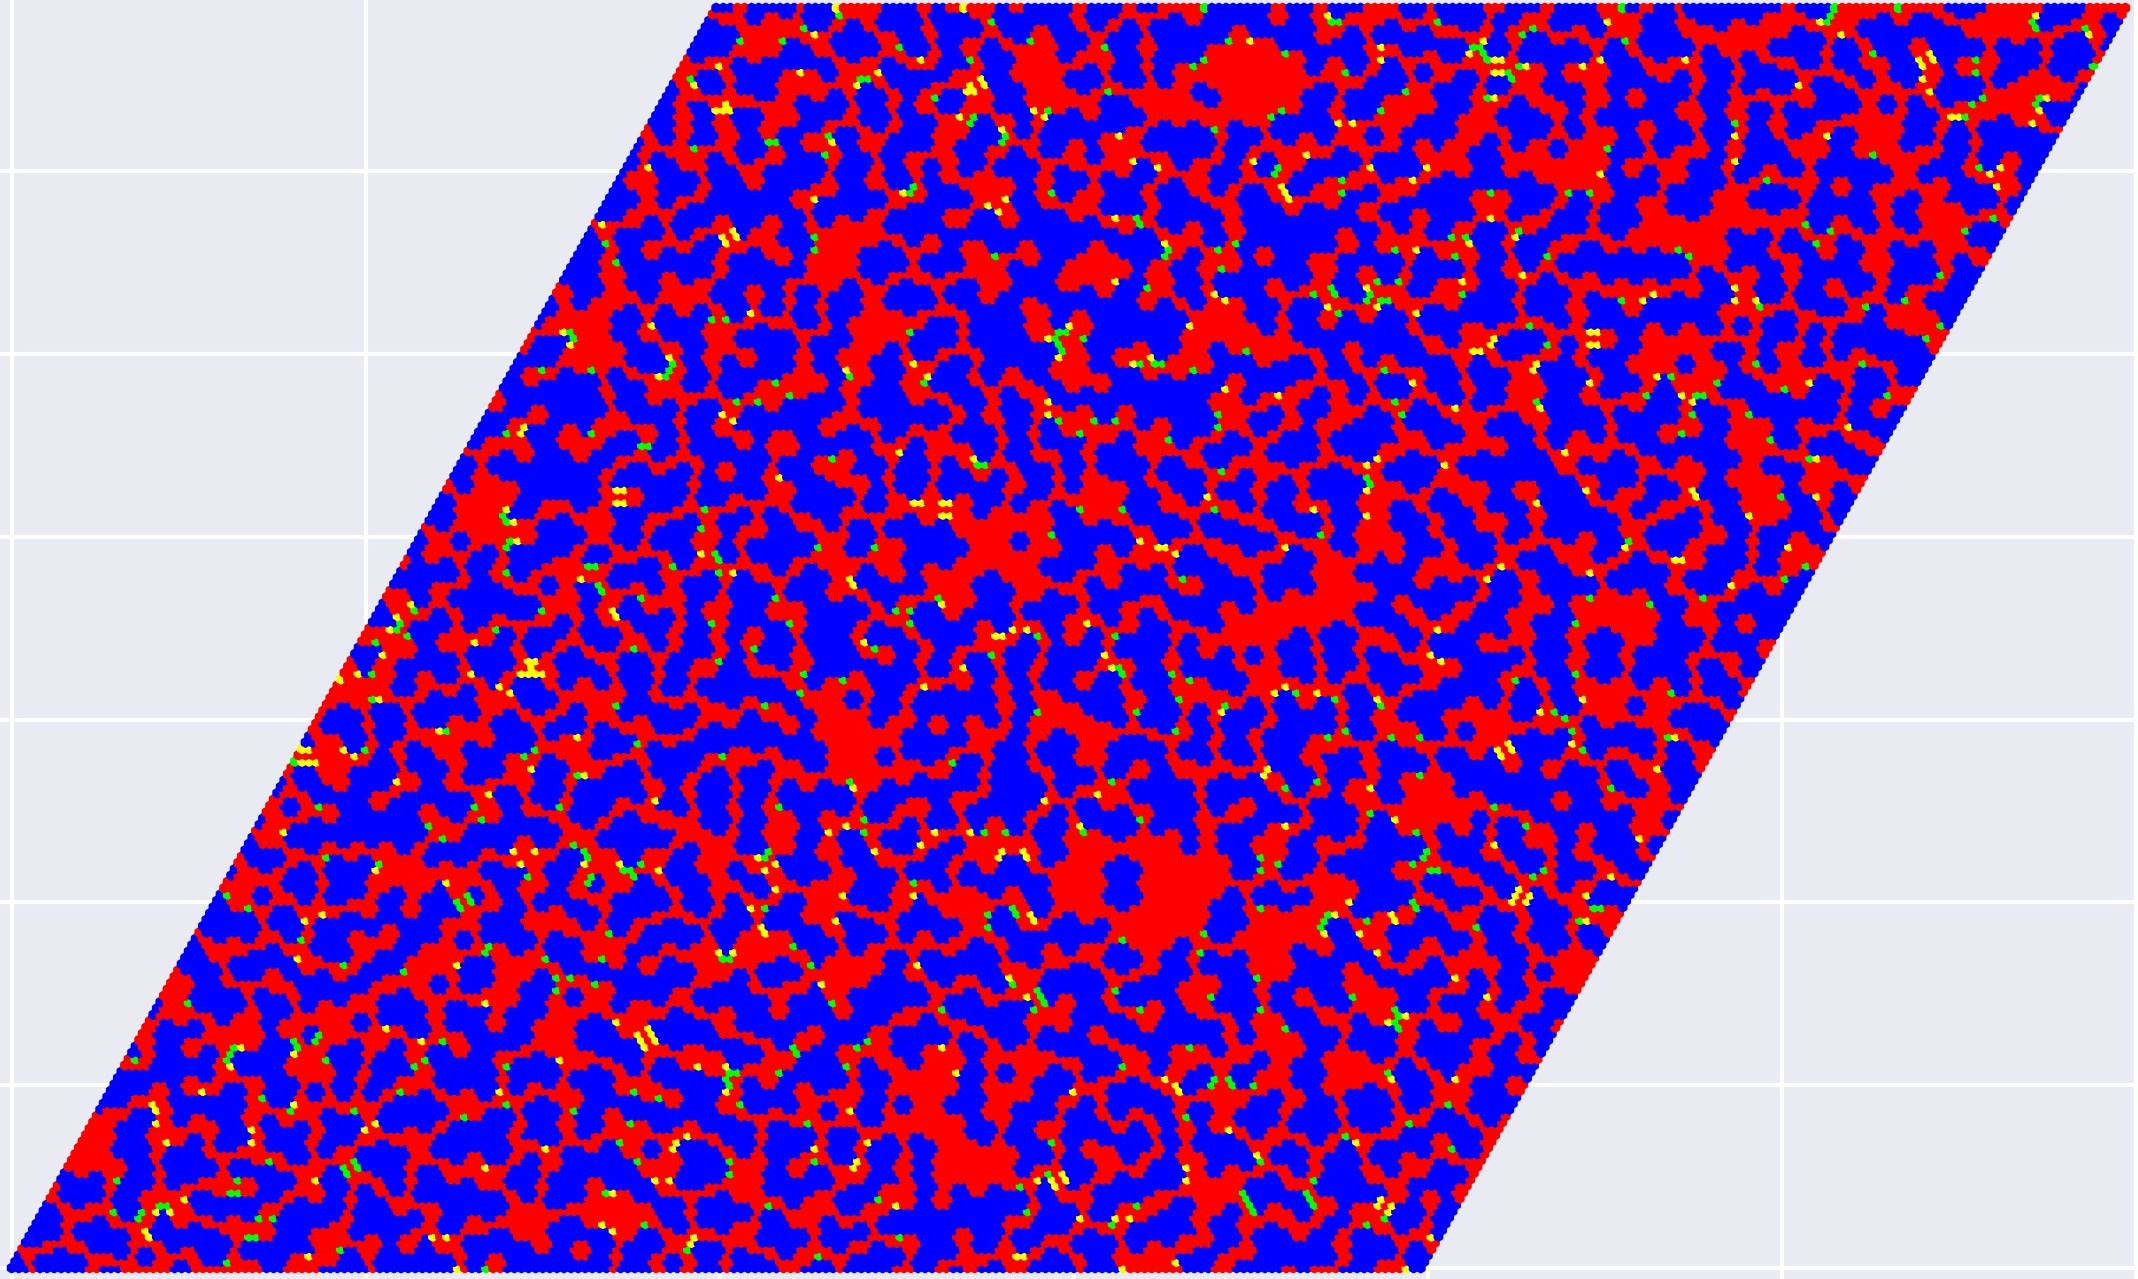
\includegraphics[width=.9\linewidth]{TriangularMeanFieldGame/triangular_snapshot_b=17.jpg}
          \caption{$b=1.7$}
          \label{fig:trsub6}
        \end{subfigure}
        
        \begin{subfigure}{.33\textwidth}
          \centering
          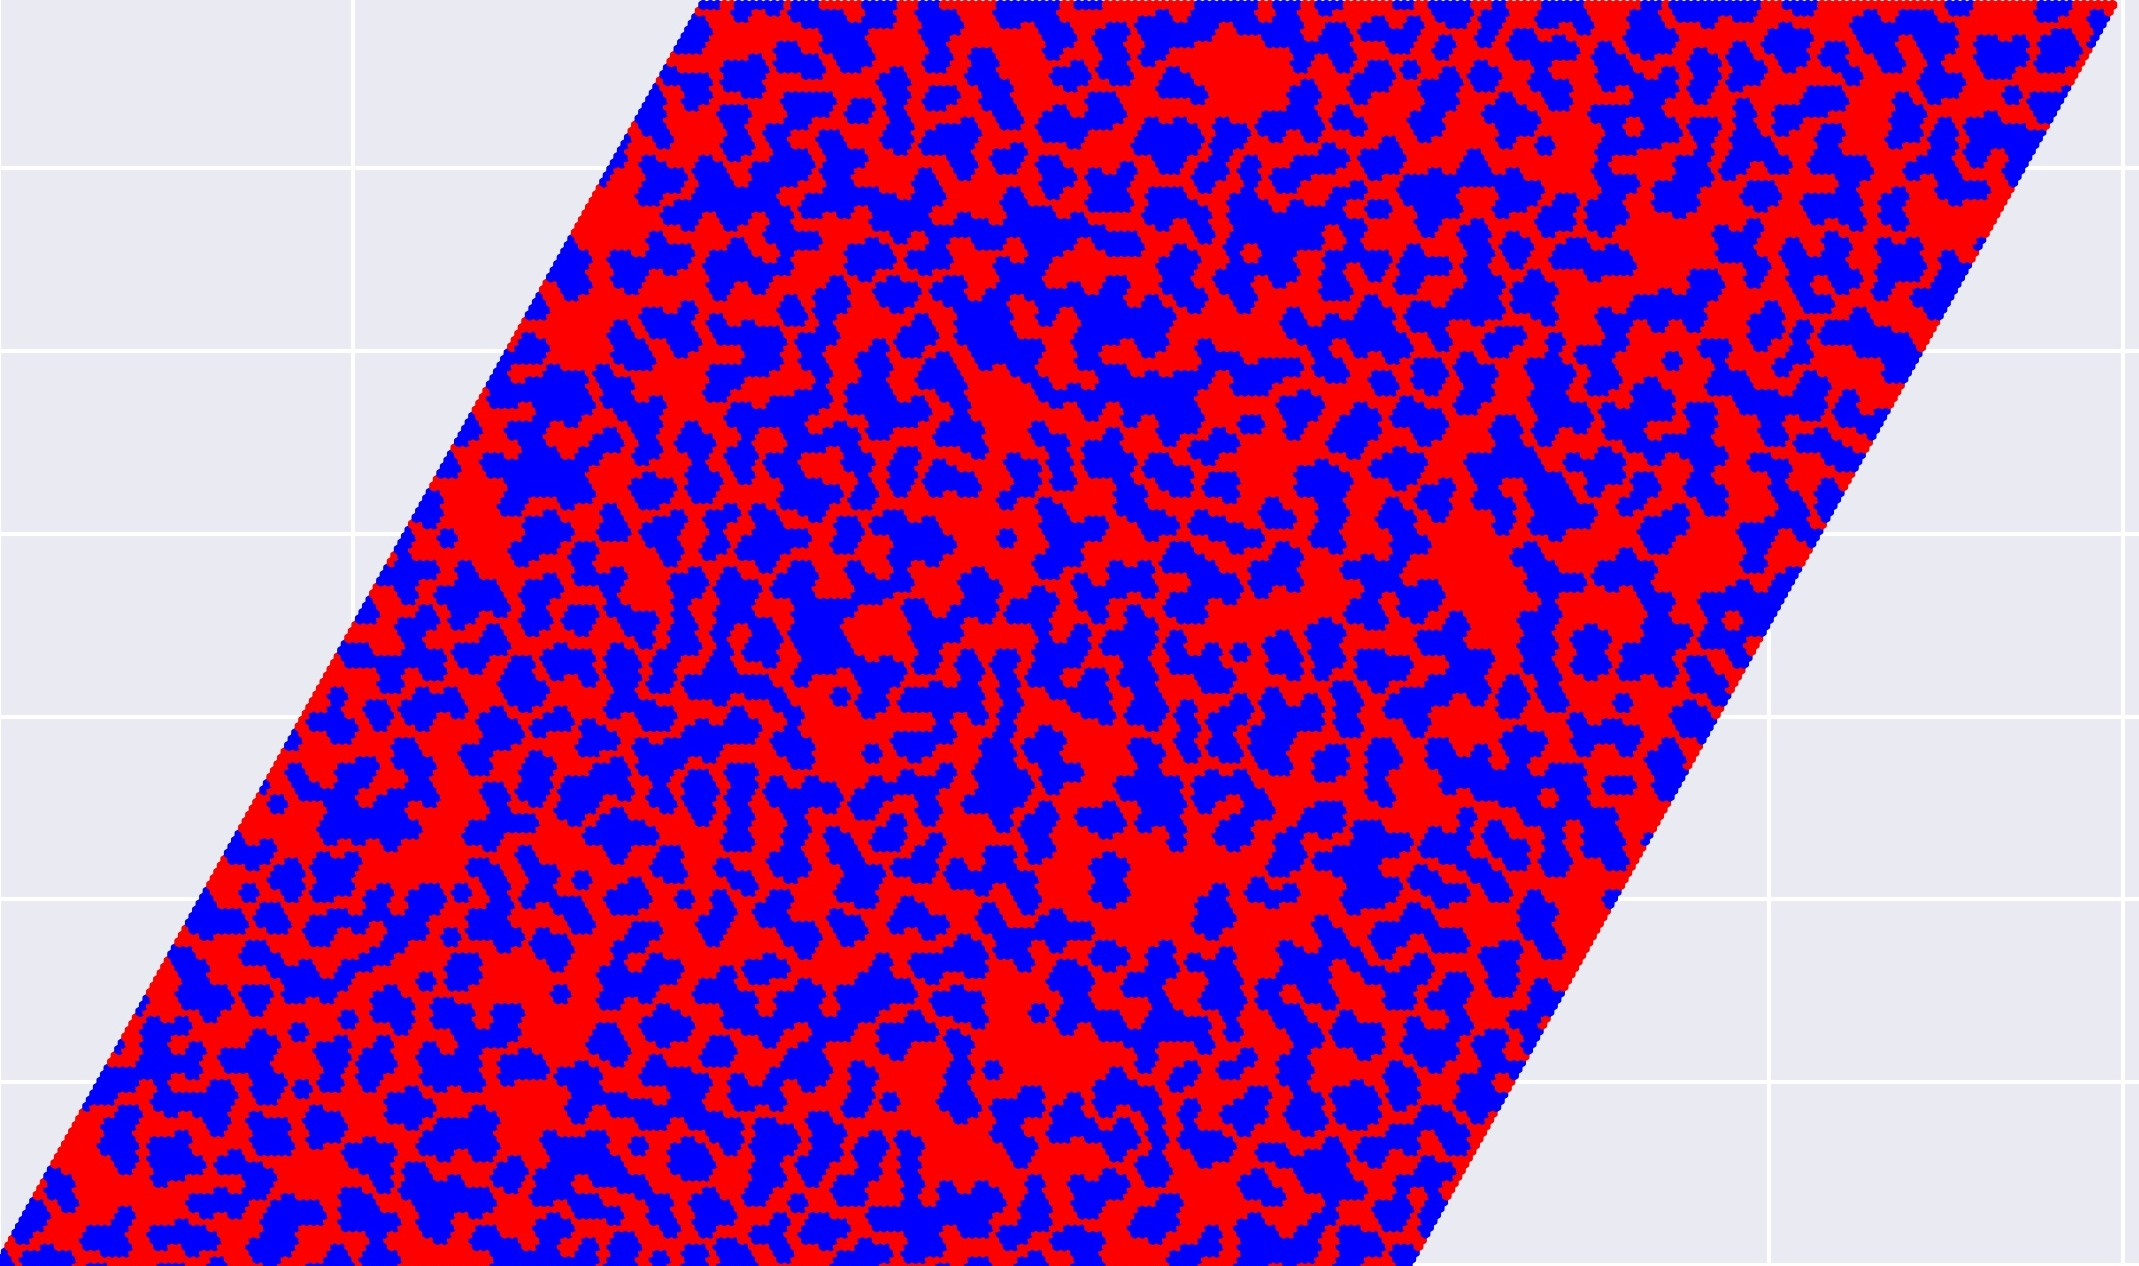
\includegraphics[width=.9\linewidth]{TriangularMeanFieldGame/triangular_snapshot_b=18.jpg}
          \caption{$b=1.8$}
          \label{fig:trsub7}
        \end{subfigure}%
        \begin{subfigure}{.33\textwidth}
          \centering
          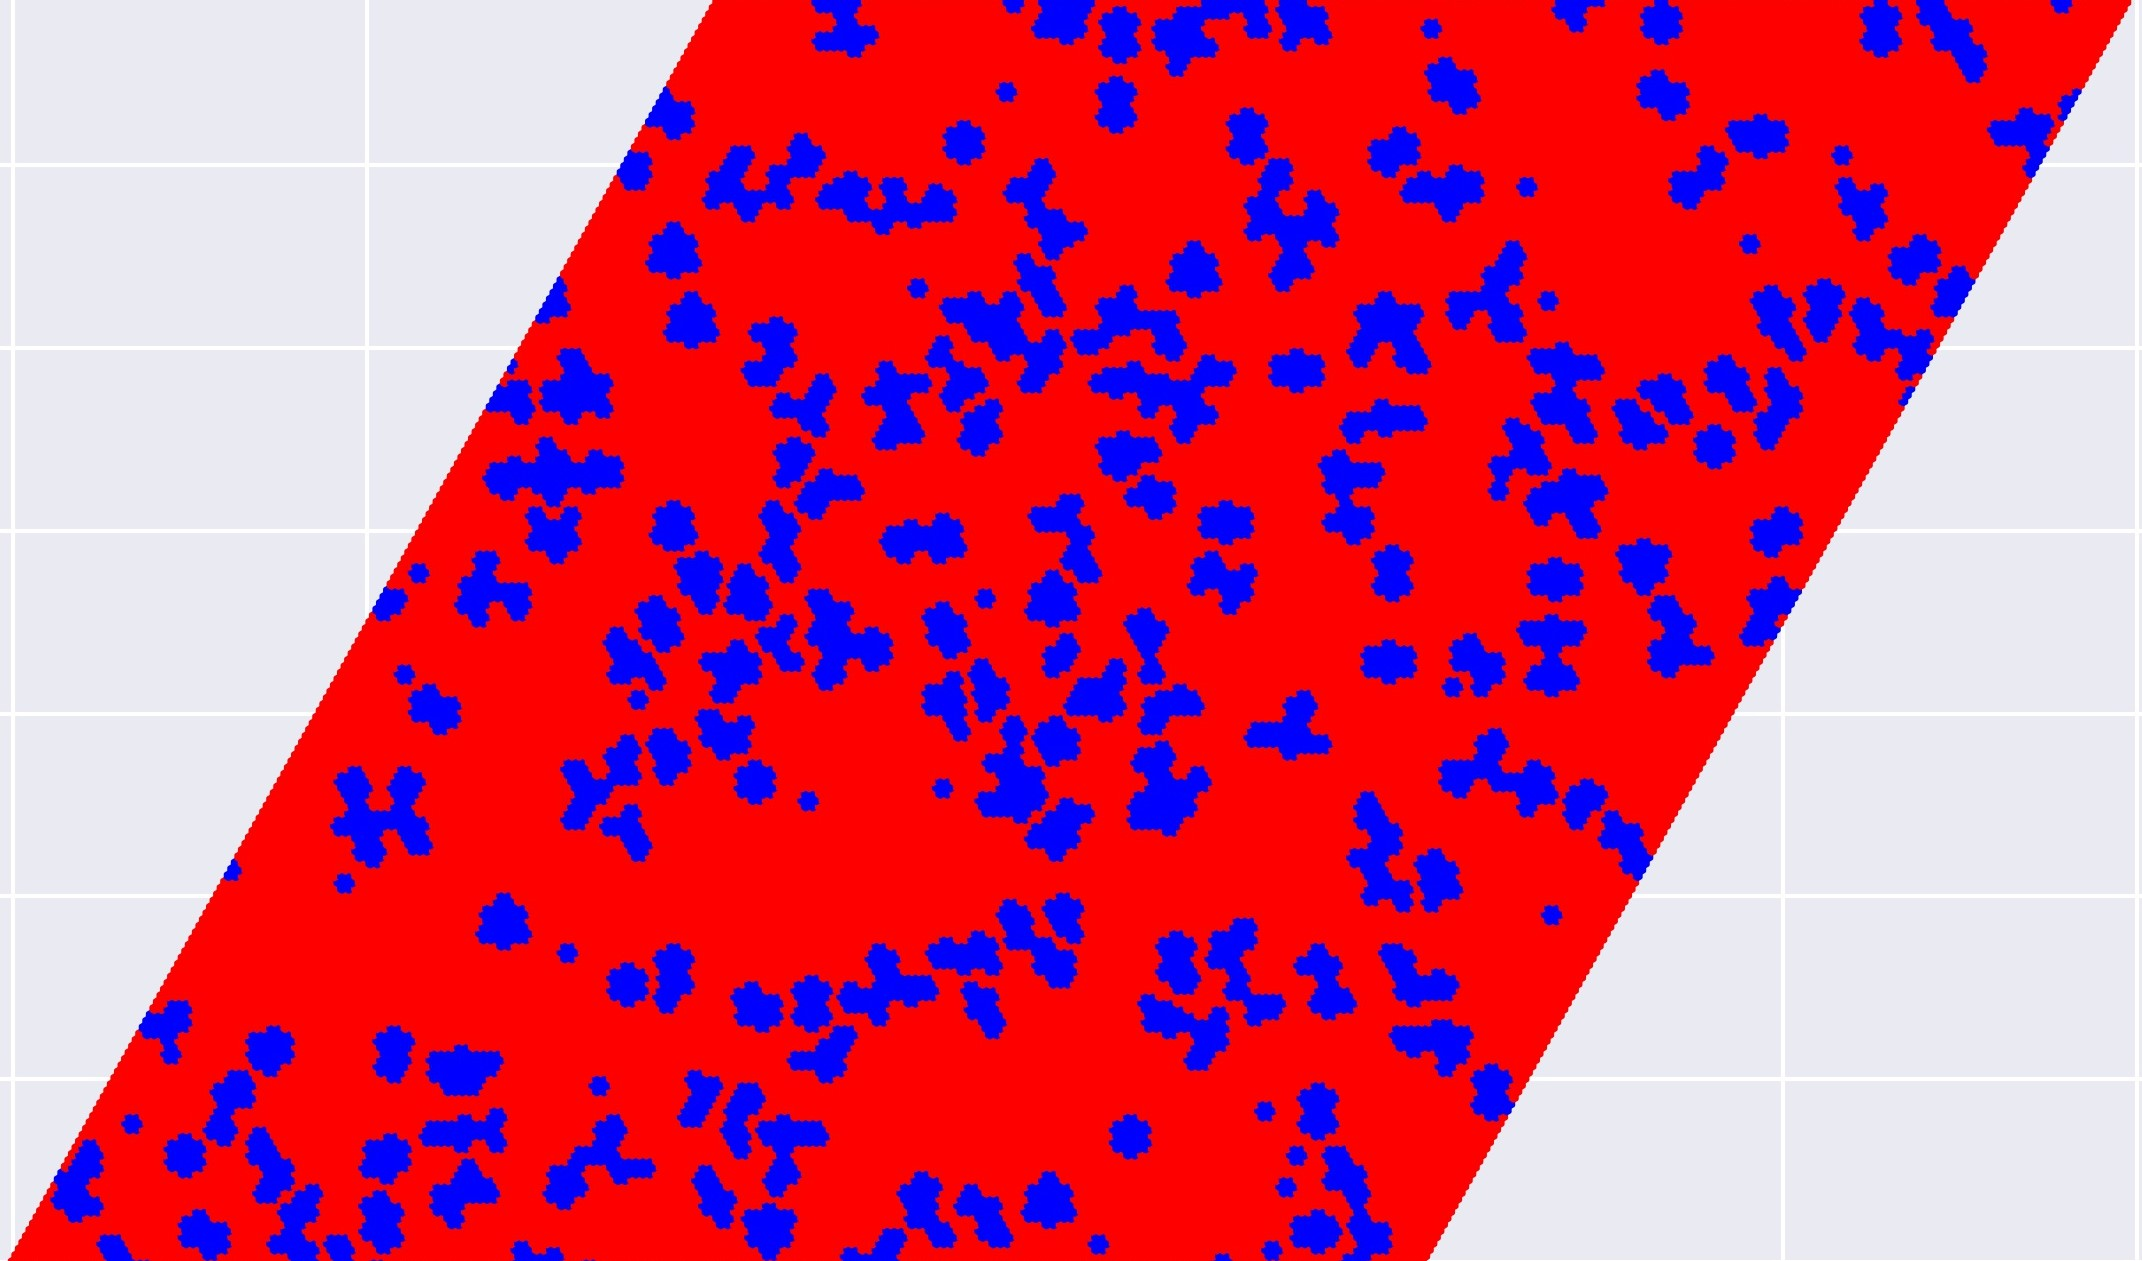
\includegraphics[width=.9\linewidth]{TriangularMeanFieldGame/triangular_snapshot_b=19.jpg}
          \caption{$b=1.9$}
          \label{fig:trsub8}
        \end{subfigure}%
        \begin{subfigure}{.33\textwidth}
          \centering
          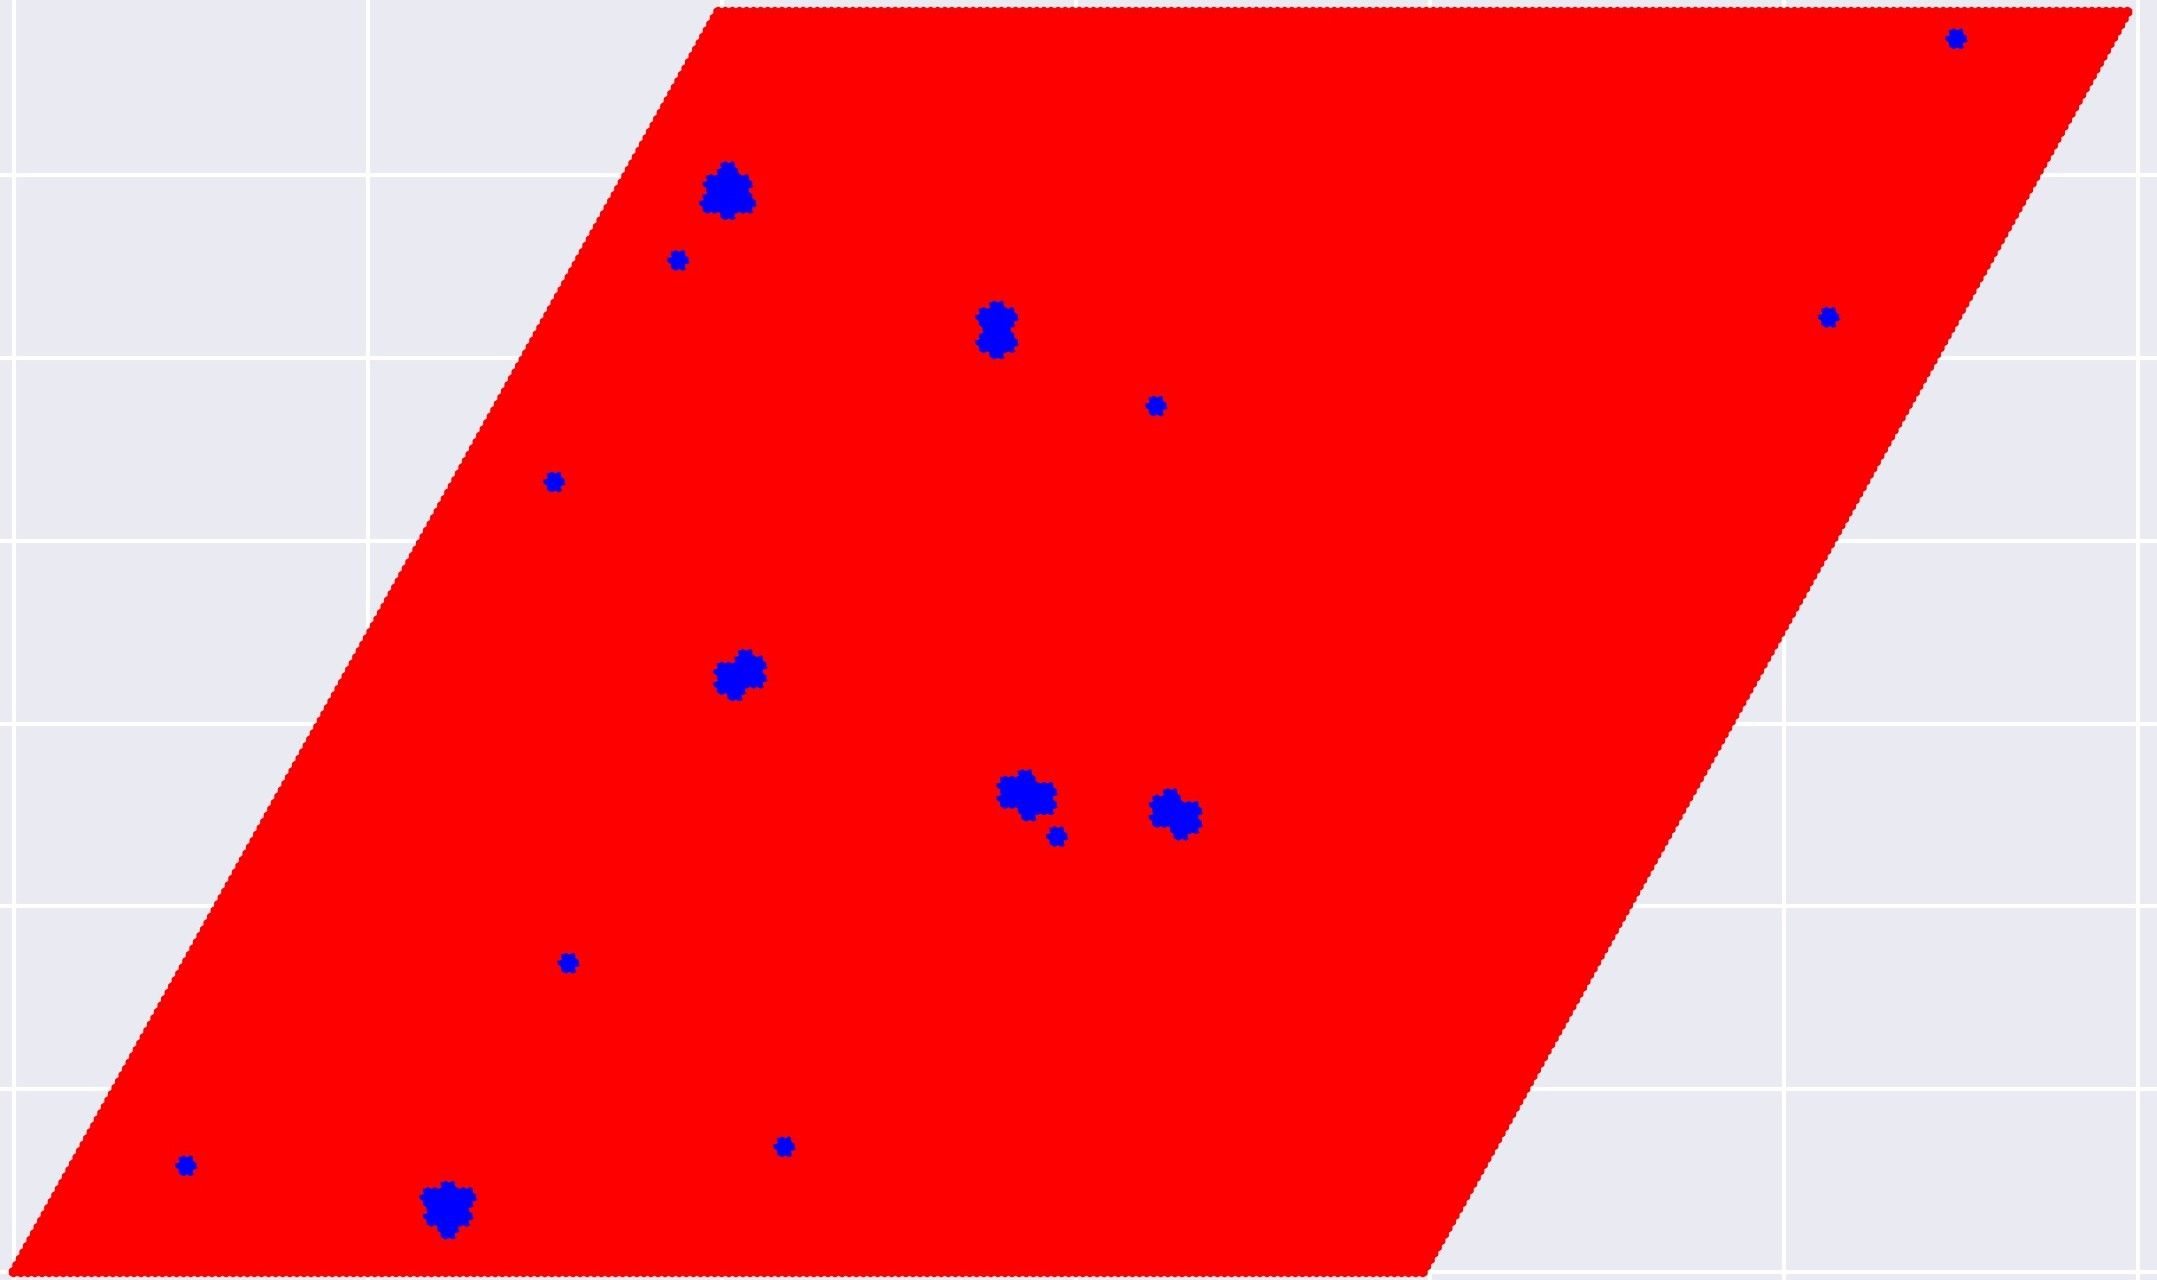
\includegraphics[width=.9\linewidth]{TriangularMeanFieldGame/triangular_snapshot_b=199.jpg}
          \caption{$b=1.99$}
          \label{fig:trsub9}
        \end{subfigure}
    
        
        \caption{ Примеры полей 200 на 200 при начальной плотности $0.9$ после 5000 шагов на треугольной решетке и игре со средним полем.\\
        Синий — кооператоры\\
        Красный — дефекторы\\
        Желтый — кооператоры, ставшие дефекторами(на данном ходе)\\
        Зеленый — дефекторы, ставшие кооператорами(на данном ходе)}
        \label{fig:triangfields}
    \end{figure}

\subsection{Коротко о треугольной решетке}
    Плотность кооператоров при игре со средним полем падает быстрее, чем при игре Новака-Мэя, но, в отличии от квадратной решетки, на треугольной решетке пропадает хаотический режим.
    
\section{Игра с двумя полями}
\subsection{Описание игры}
    Рассмотрим два поля размера $L\times L$, на которых агенты играют в модификацию игры со средним полем с выигрышами $b_1$ и $b_2$ соответственно. Плотность кооператоров на полях равна $f_1$ и $f_2$. Модификация игры заключается в том, что вместо игры со средним кооператором на этом же самом поле, он играет против среднего кооператора с другого поля.(В таблице \ref{tab:2} представлен выигрыш агента с поля 1, при игре против агента с поля 2)

  
  \begin{minipage}{\linewidth}
    \centering
    \captionof{table}{Выигрыш агента при игре с соседями} \label{tab:1} 
    \setlength{\extrarowheight}{2pt}
    \begin{tabular}{cc|c|c|}
      & \multicolumn{1}{c}{} & \multicolumn{2}{c}{Агент}\\
      & \multicolumn{1}{c}{} & \multicolumn{1}{c}{$\mathcal{D}$}  & \multicolumn{1}{c}{$\mathcal{C}$} \\\cline{3-4}
      \multirow{2}*{Сосед}  & $\mathcal{D}$ & $0$ & $0$ \\\cline{3-4}
      & $\mathcal{C}$ & $b_1$ & $1$ \\\cline{3-4}
    \end{tabular}
    \end{minipage}
    
    \begin{minipage}{\linewidth}
    \centering
    \captionof{table}{Выигрыш агента с первого поля при игре против среднего кооператора со второго поля} \label{tab:2} 
    \setlength{\extrarowheight}{2pt}
    \begin{tabular}{cc|c|c|}
      & \multicolumn{1}{c}{} & \multicolumn{2}{c}{Агент}\\
      & \multicolumn{1}{c}{} & \multicolumn{1}{c}{$\mathcal{D}$}  & \multicolumn{1}{c}{$\mathcal{C}$} \\\cline{3-4}
      \multirow{2}*{Сосед}  & $\mathcal{D}$ & $0$ & $0$ \\\cline{3-4}
      & $\mathcal{C}$ & $b_1 f_2$ & $f_2$ \\\cline{3-4}
    \end{tabular}
    \end{minipage}
  
\subsection{Как считались данные}
    Для моделирования было сгенерировано 40 различных пар начальных полей $100\times100$ с начальной плотностью кооператоров равной $0.9$. В каждой паре полей оба поля были идентичными.
    Моделирование проводилось на парах $(b_1,\;b_2)$, где $b_2 \geq b_1$ и $b_1,\;b_2$ брались из интервала $[0.9, 2.0]$. Значение $\frac{f_1+f_2}{2}$ рассчитывалось как средняя плотность 40 полей с 10000 до 16000 шага.
    Так как оба поля в начальный момент времени совпадают, то поведение на первом и втором поле при параметрах $(b_1,\;b_2)$ будет совпадать с поведением на втором и первом поле соответственно при параметрах $(b_2, b_1)$, что было использовано при моделировании.
    
\subsection{Что не ожидаем увидеть?}
    Для начала обсудим, какие значения $\frac{f_1+f_2}{2}$ мы \textbf{не ожидаем} увидеть. Так как плотность кооператоров на первом поле зависит от распределения кооператоров на поле и плотности кооператоров на втором поле, то $f_1$ должно отличаться от плотности, если бы поля "не взаимодействовали". Аналогичные рассуждения верны для $f_2$. Предположим что это не так, тогда $\frac{f_1+f_2}{2}$ будет принимать значения, показанные на рис.
     \ref{fig:wrong}
    
    \begin{figure}[H]
         \centering
         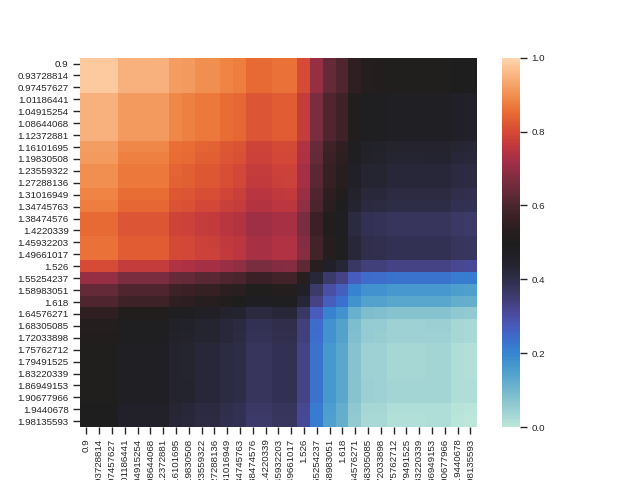
\includegraphics[width=0.95\columnwidth, keepaspectratio=True]{DoubleField/wrong.png}
         \caption{Средняя плотность кооператоров на несвязанных полях. Цветом отмечена средняя плотность на двух полях. Данные показаны для точек, отличных от точек на других рисунках.}
         \label{fig:wrong}
    \end{figure}

\subsection{Результаты моделирования}
    На рисунках \ref{fig:right}, \ref{fig:many} и \ref{fig:3d} показана зависимость $\frac{f_1+f_2}{2}$ от параметра выигрыша. 
    При сравнении рис. \ref{fig:wrong} и \ref{fig:right} хорошо видно, что при игре на связанных полях происходит более резкий переход, в сравнении с игрой на несвязанных полях. Особенно хорошо переход виден на рис. \ref{fig:3d}\footnote{Почему-то в первый раз форма графика напомнила висячие сады или фермы в горах(не помню название технологии)}. Для более конкретных выводов требуются данные из большего числа точек.
    
    На рис. \ref{fig:twoden} показана плотность на первом и втором полях. Можно заметить, что при "больших" и "маленьких" значениях выигрыша, плотность кооператоров на соответствующем поле не зависит от выигрыша на другом. На рис. \ref{fig:3df1} показана плотность кооператоров на первом поле.
    \begin{figure}[H]
         \centering
         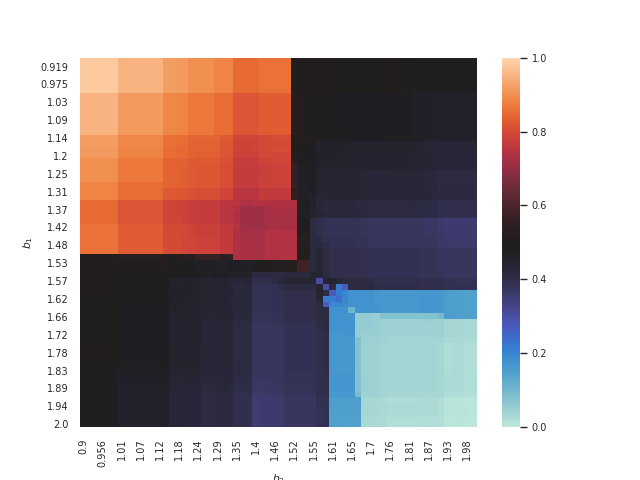
\includegraphics[width=0.7\columnwidth, keepaspectratio=True]{DoubleField/right.png}
         \caption{Средняя плотность кооператоров на \textbf{связанных} полях. Цветом отмечена средняя плотность на двух полях. $b_1$ по вертикали, $b_2$ по горизонтали.}
         \label{fig:right}
    \end{figure}
    \begin{figure}[H]
         \centering
         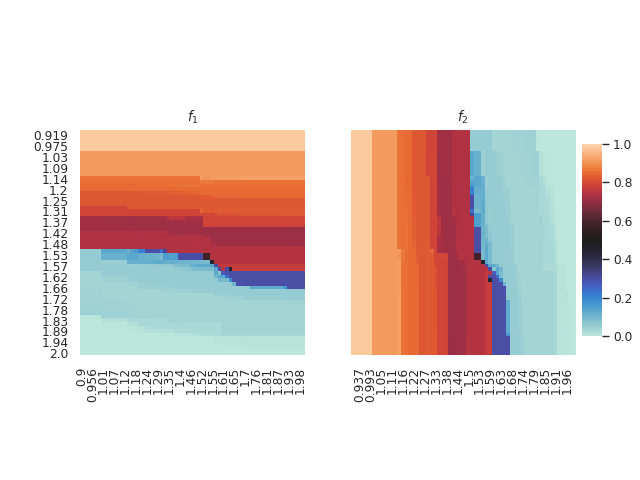
\includegraphics[width=0.95\columnwidth, keepaspectratio=True]{DoubleField/twodensity.png}
         \caption{Плотность кооператоров на первом и втором поле. $b_1$ по вертикали, $b_2$ по горизонтали.}
         \label{fig:twoden}
    \end{figure}
    
    \begin{figure}[H]
         \centering
         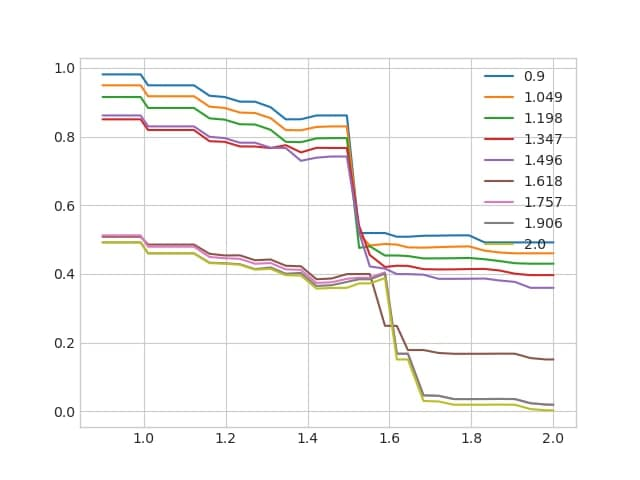
\includegraphics[width=0.95\columnwidth, keepaspectratio=True]{DoubleField/many.jpg}
         \caption{Зависимость средней плотности кооператоров от $b_2$ при фиксированном значении $b_1$.}
         \label{fig:many}
    \end{figure}
    \begin{figure}[H]
         \centering
         \begin{minipage}{.45\linewidth}
          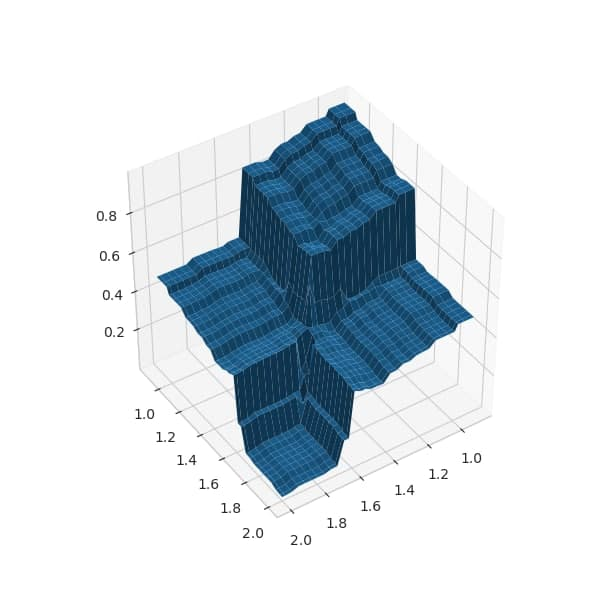
\includegraphics[width=0.95\columnwidth, keepaspectratio=True]{DoubleField/3d.jpg}
          \captionof{figure}{Средняя плотность кооператоров на связанных полях. Тоже самое, что и рис. \ref{fig:right}, но визуализированное по другому.}
         \label{fig:3d}
        \end{minipage}
        \hspace{.05\linewidth}
        \begin{minipage}{.45\linewidth}
          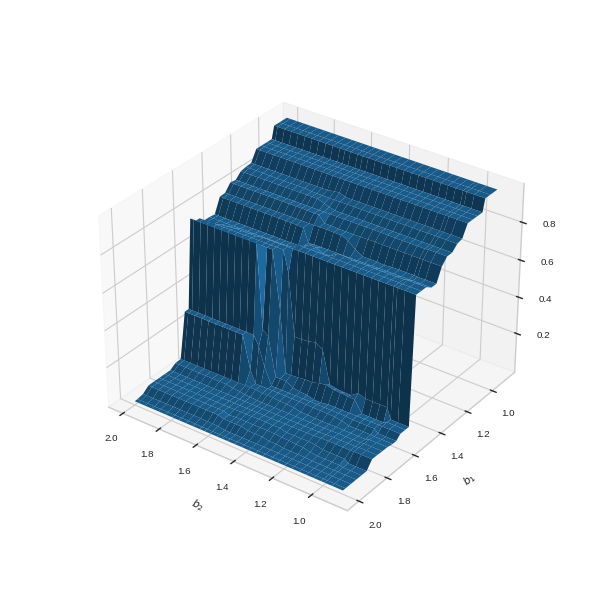
\includegraphics[width=0.95\columnwidth, keepaspectratio=True]{DoubleField/3df1.png}
         \captionof{figure}{Плотность кооператоров на первом поле.}
         \label{fig:3df1}
        \end{minipage}
    \end{figure}

\subsection{Persistence}
    Чтобы посмотреть на поведение игры при различных значениях выигрыша мы посчитали persistence. Полученные данные отображены на рис. \ref{fig:persDouble}.
    Около крайних значений параметра выигрыша($0.9,\;2$) значение $persistence$ на поле никак не зависит от выигрыша на другом поле, но при остальных значениях от параметра выигрыша на втором поле зависит наличие хаотического режима на первом поле и наоборот.
    
    На рис. \ref{fig:somepers} показана зависимость $persistence$ на втором поле от $b_2$ при некоторых значениях $b_1$. При определенных значениях $b_1$ можно наблюдать возникновение хаотического режима в одной точке.
    Чтобы прояснить поведение в данной точке было взято несколько значений $b_1$ вокруг данной точки и для них был посчитан persistence при 1000, 2000, 10000 и 15000 шагах. Я не привожу графики для последних трех, так как они полностью совпадают с 1000.(рис. \ref{fig:smallpers})
    
    \begin{figure}[H]
         \centering
         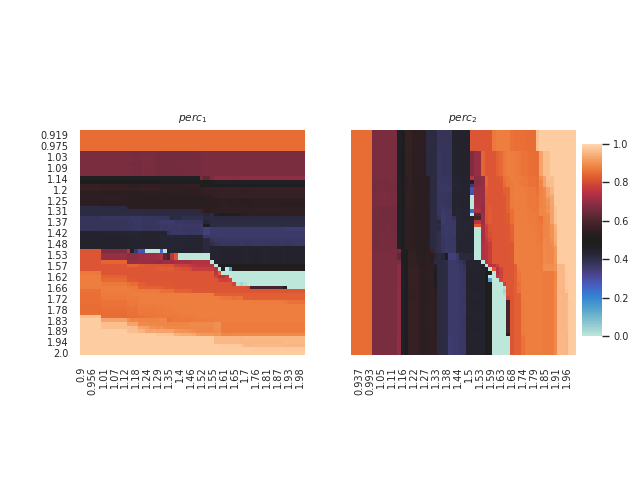
\includegraphics[width=0.95\columnwidth, keepaspectratio=True]{DoubleField/persistence.png}
         \caption{persistence на первом и втором полях.}
         \label{fig:persDouble}
    \end{figure}
    \begin{figure}[H]
         \centering
         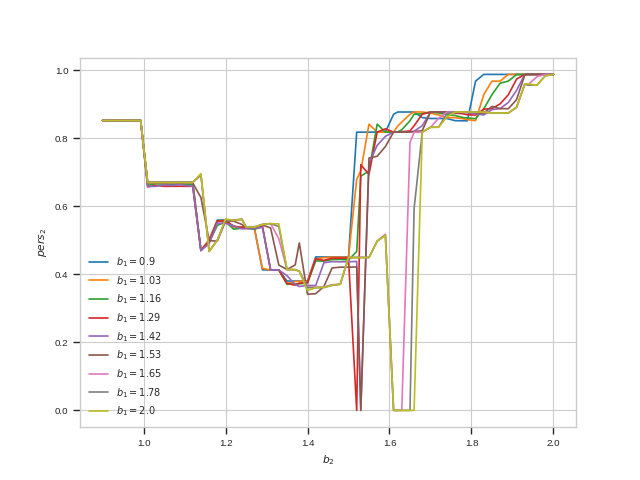
\includegraphics[width=0.95\columnwidth, keepaspectratio=True]{DoubleField/somepersistence.png}
         \caption{persistence на втором поле при различных $b_1$.}
         \label{fig:somepers}
    \end{figure}
    
    \begin{figure}[H]
         \centering
         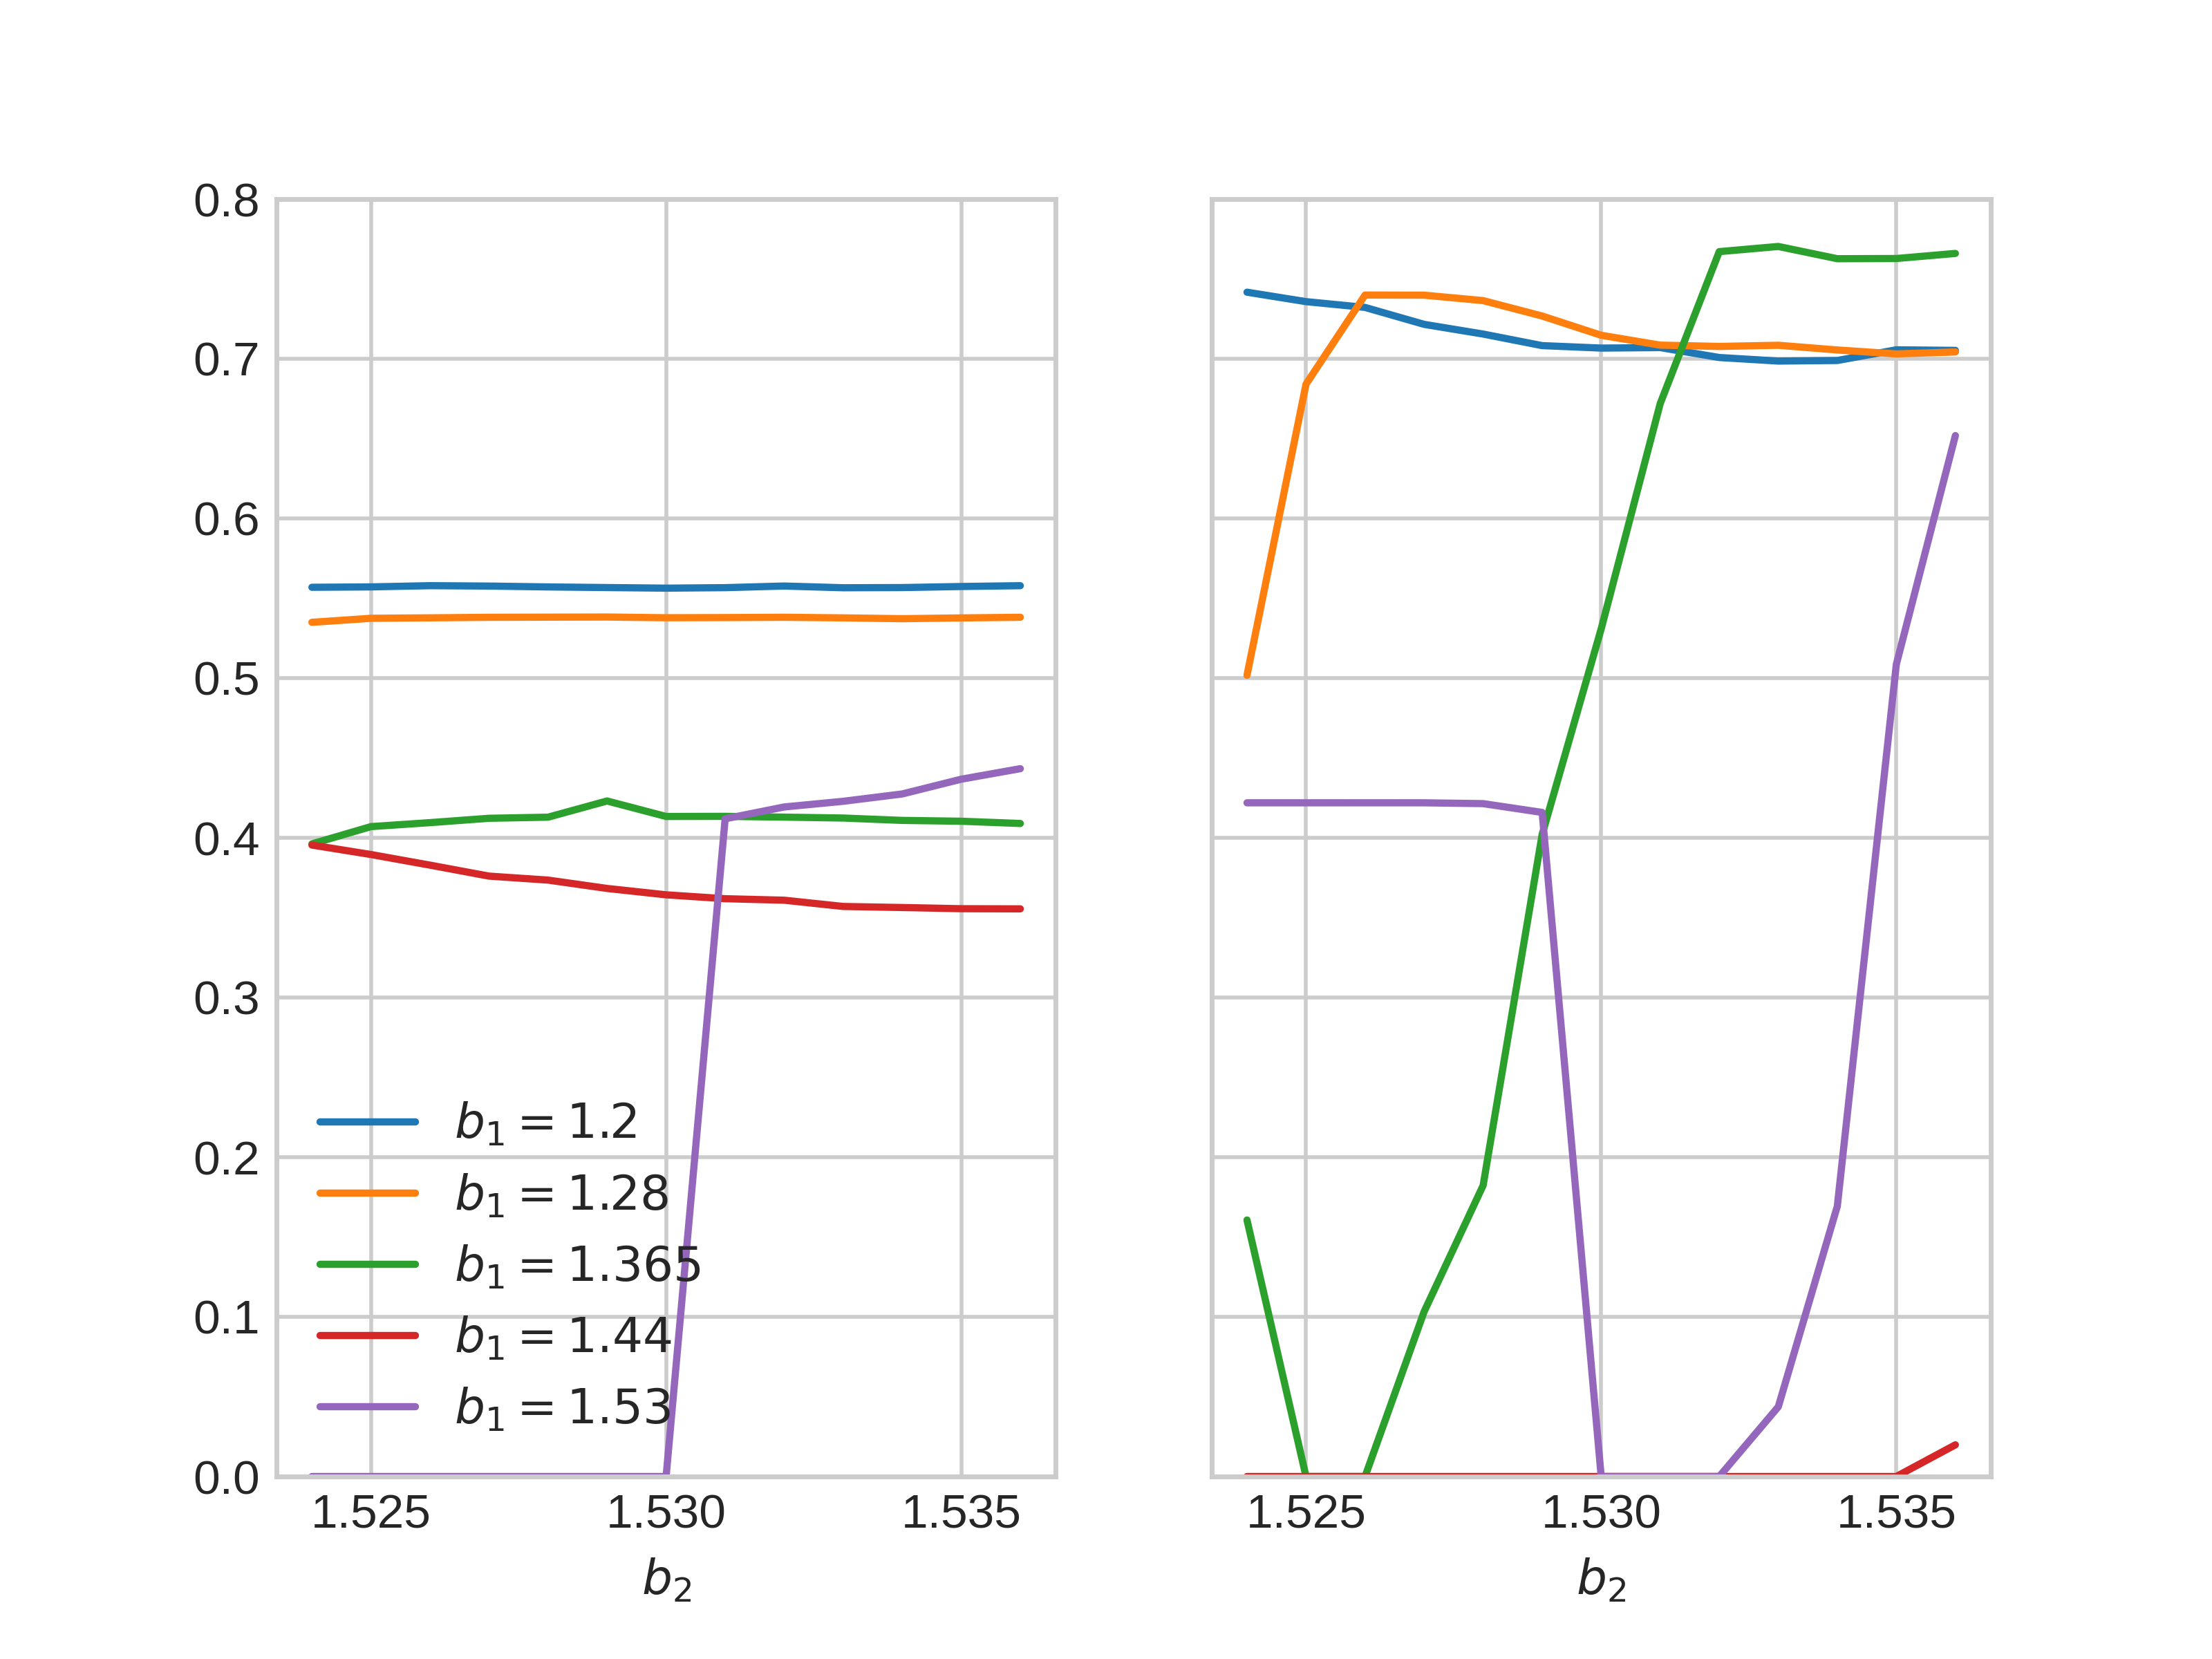
\includegraphics[width=0.95\columnwidth, keepaspectratio=True]{DoubleField/persistence_at_b_2_153.png}
         \caption{persistence на первом и втором поле при различных $b_1$ около $b_2=1.53$.}
         \label{fig:smallpers}
    \end{figure}

\subsubsection{Смена persistence}
    \label{sec:persistence}
    Наиболее интересным случаем для рассмотрения является $b_1=1.53$. При $b_2 < 1.53$ на первом поле агенты находятся в "хаотическом режиме" с крупными кластерами кооператоров(синее), в то время как на втором поле дефекторы образуют сеть каналов, с крупными кластерами кооператоров. При $b_2=1.53$ агенты на обоих полях находятся в хаотическом режиме с небольшими кластерами кооператоров и дефекторов.
    При $b_2 > 1.53$ ситуация на полях меняется и на первом поле дефекторы образуют сеть каналов, а на втором поле агенты находятся в хаотическом режиме с крупными кластерами кооператоров.(рис. \ref{fig:DfieldsFixb1})
    
    Похожий переход для значения $b_1=1.56$ представлен ниже(см. \ref{sec:configs})
    
    \begin{figure}[H]
         \centering
         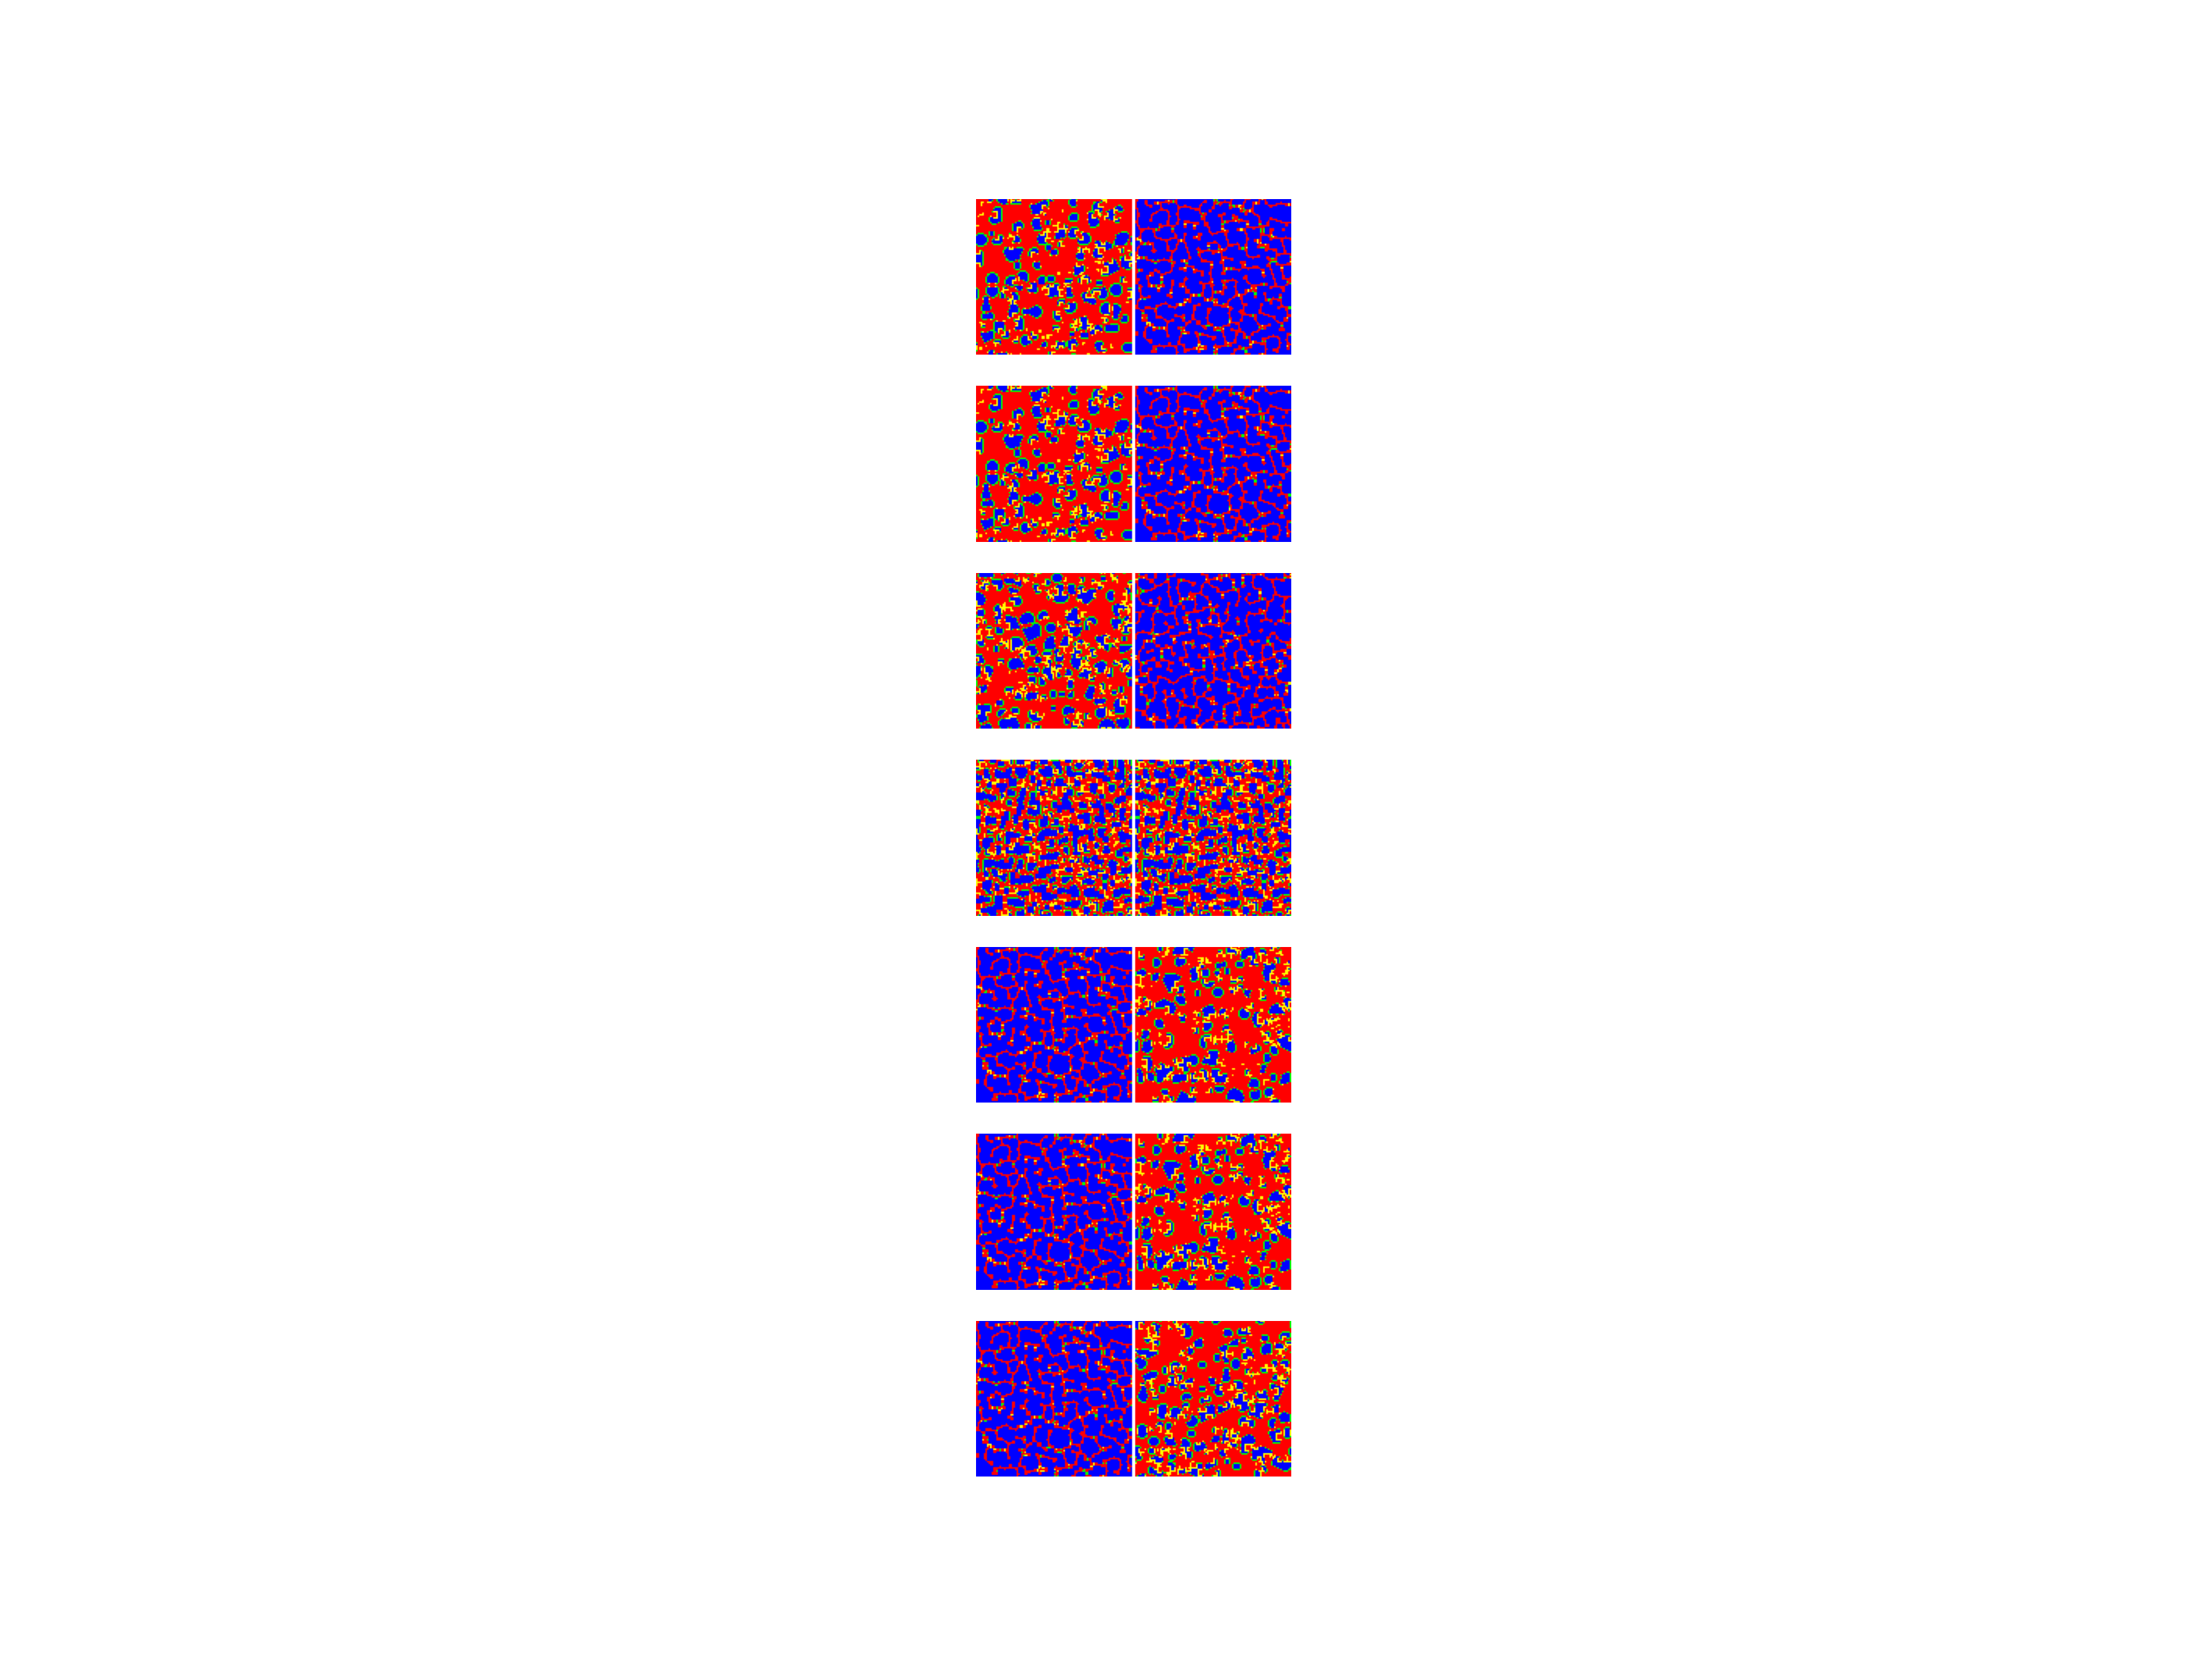
\includegraphics[width=0.95\columnwidth, keepaspectratio=True]{DoubleField/colored_2fields153.png}
         \caption{Окрашенные поля при $b_1=1.53$ и $b_2=1.527, 1.528, 1.529, 1.53, 1.531, 1.532, 1.533$}
         \label{fig:DfieldsFixb1}
    \end{figure}

\subsubsection{Persistence вблизи диагонали с хаосом}
    Для более подробного изучения перехода был рассмотрен $persistence$ на втором поле при значениях, близких к хаотическому режиму при игре на одном поле. На рис. \ref{fig:chaos_pers}, \ref{fig:chaos_pers_small} показано значение $persistence$ при смещении на $\Delta$ перпендикулярно диагонали в точке $(b,\;b)$. Как видно из графика, при проходе через диагональ $persistence$ меняется скачком. Те при $\Delta\neq0$(при большинстве значений) большинство агентов не меняет свою стратегию и "стабильны", но при $\Delta=0$ наступает режим "хаоса" и все агенты меняют свою стратегию. Существуют значения параметра выигрыша, при которых либо с одной, либо с обеих сторон сохраняется хаос, но при отдалении от диагонали он пропадает таким же резким скачком.
    \begin{figure}[H]
         \centering
         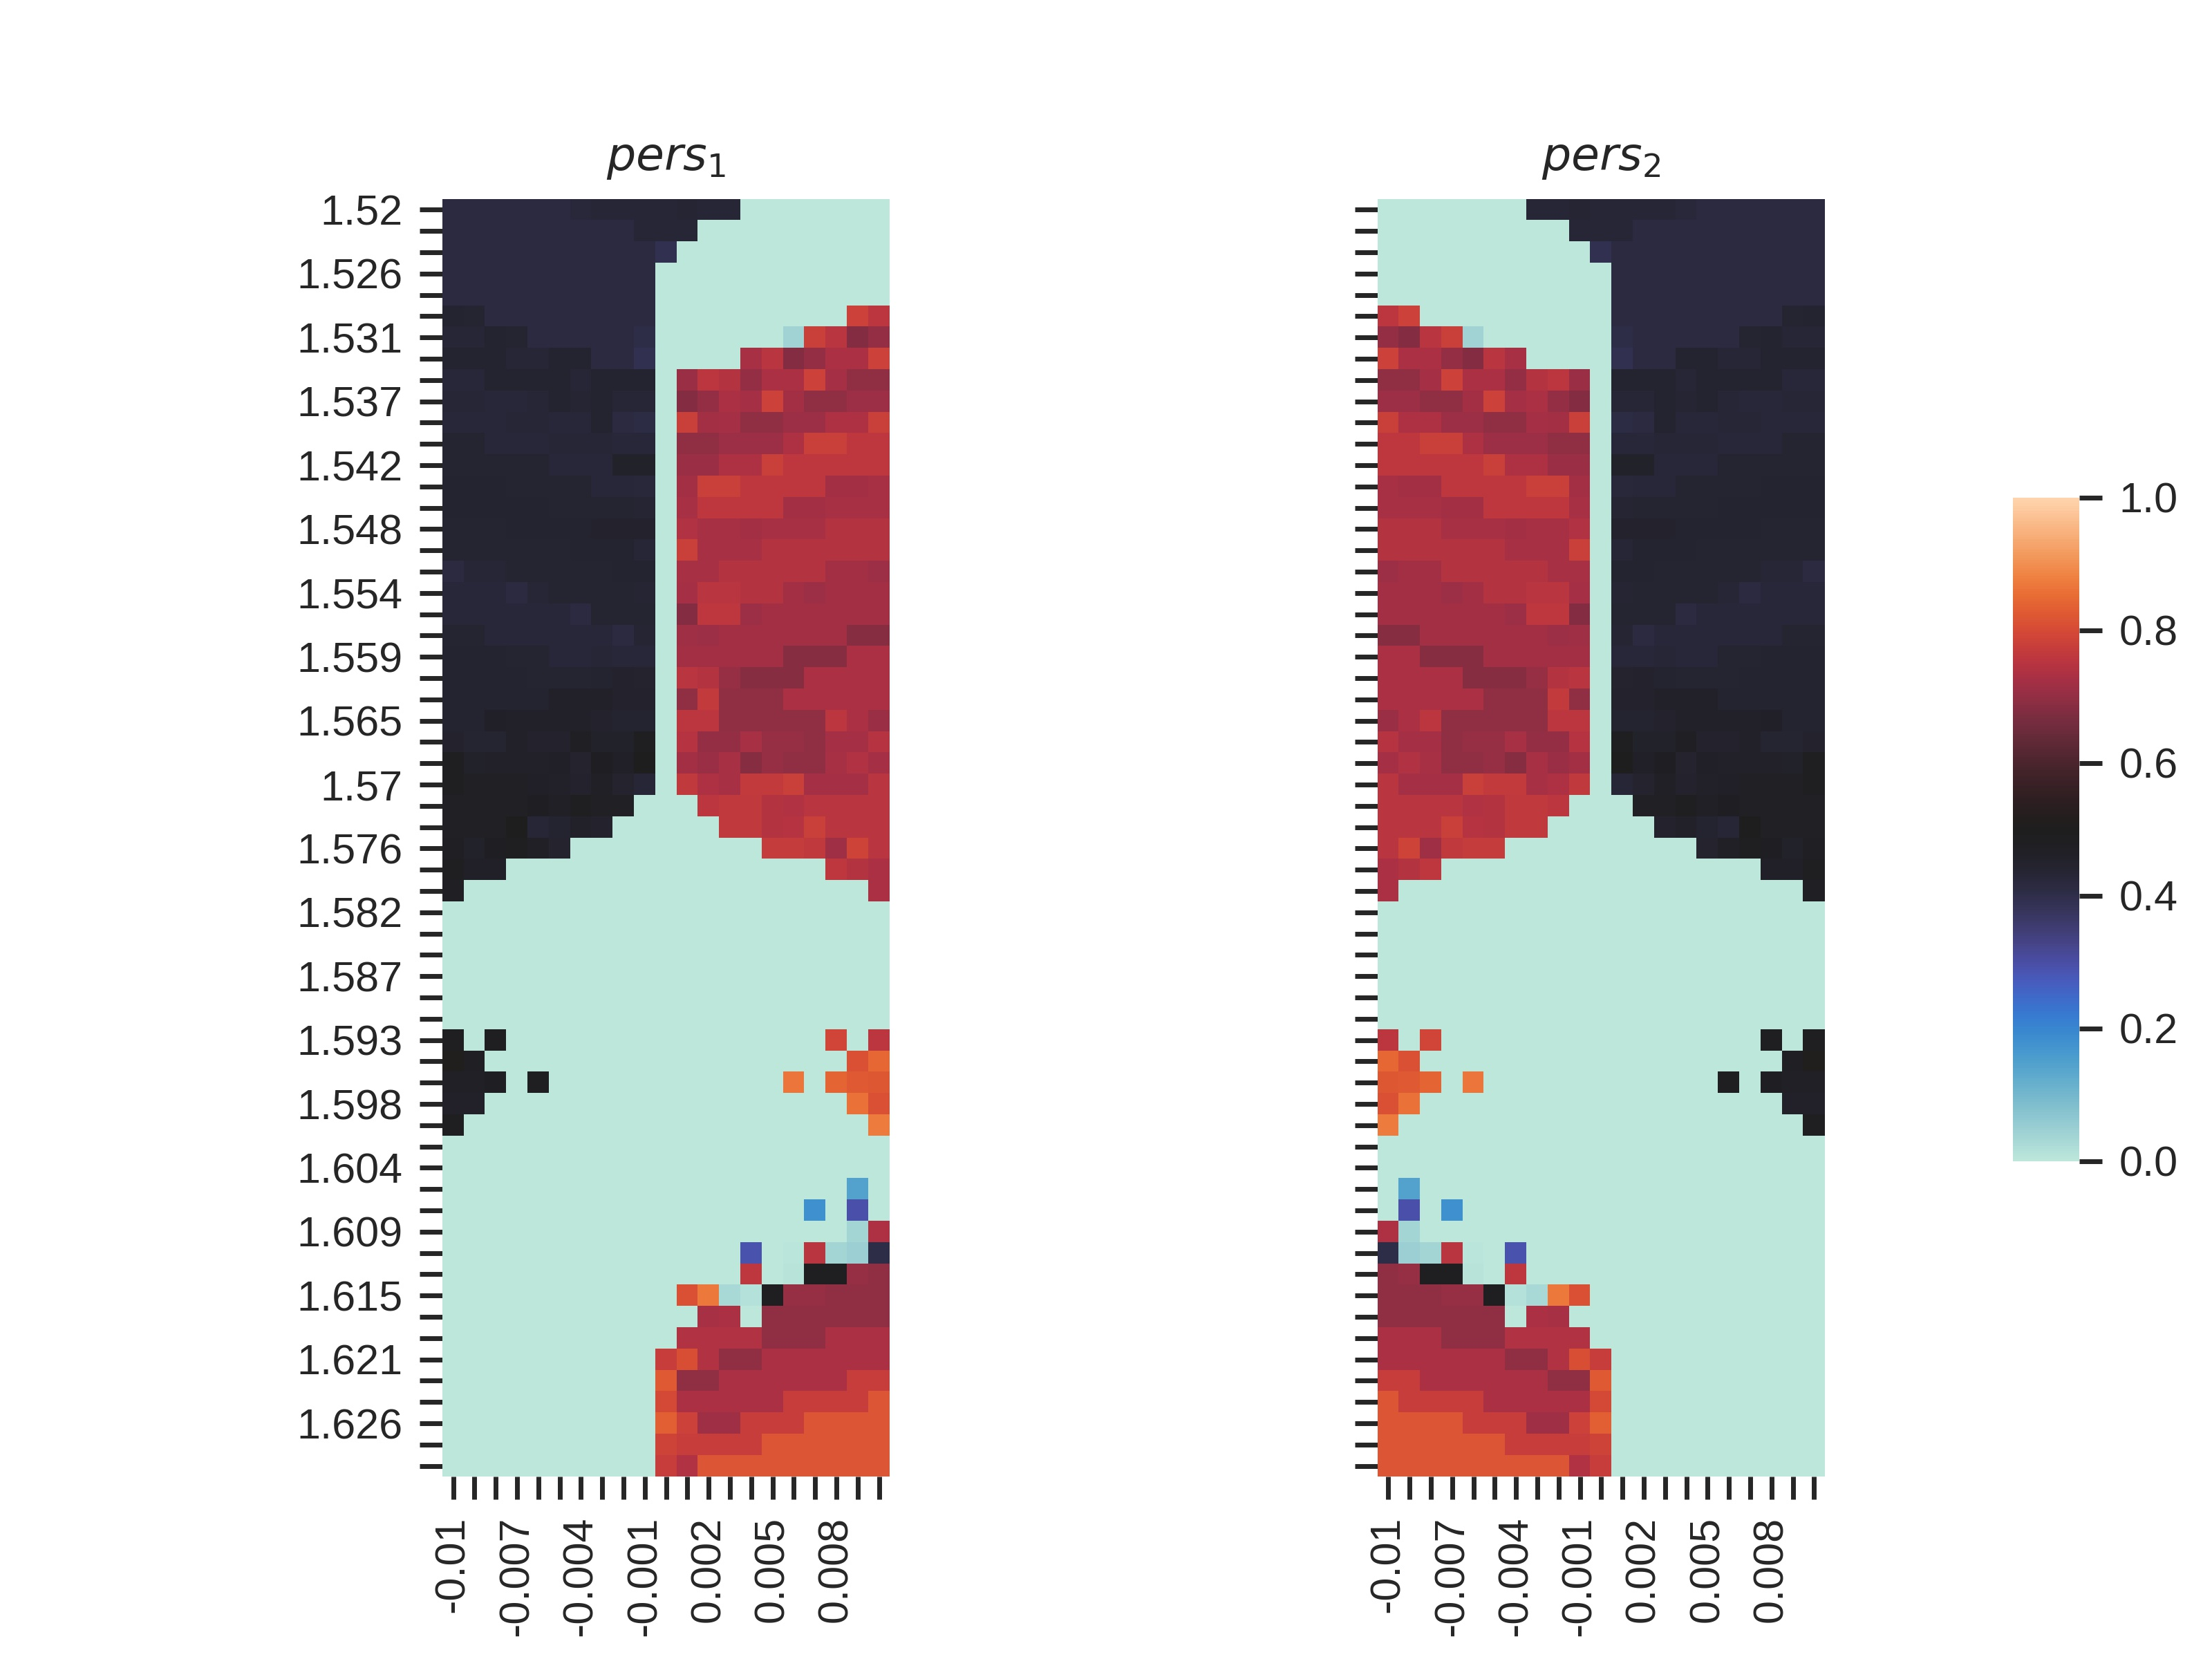
\includegraphics[width=0.95\columnwidth, keepaspectratio=True]{DoubleField/double_field_persistence_diag.jpg}
         \caption{Persistence на первом и втором поле вблизи диагонали $(b, b)$. По вертикальной оси значение $b$, по горизонтали расстояние от диагонали $\Delta$ ($(b_1,\;b_2) = (b,\;b) + (1/\sqrt{2},\;-1/\sqrt{2})\Delta$). Цветом обозначен $persistence$. $\Delta$ с шагом $0.001$}
         \label{fig:chaos_pers}
    \end{figure}
    \begin{figure}[H]
         \centering
         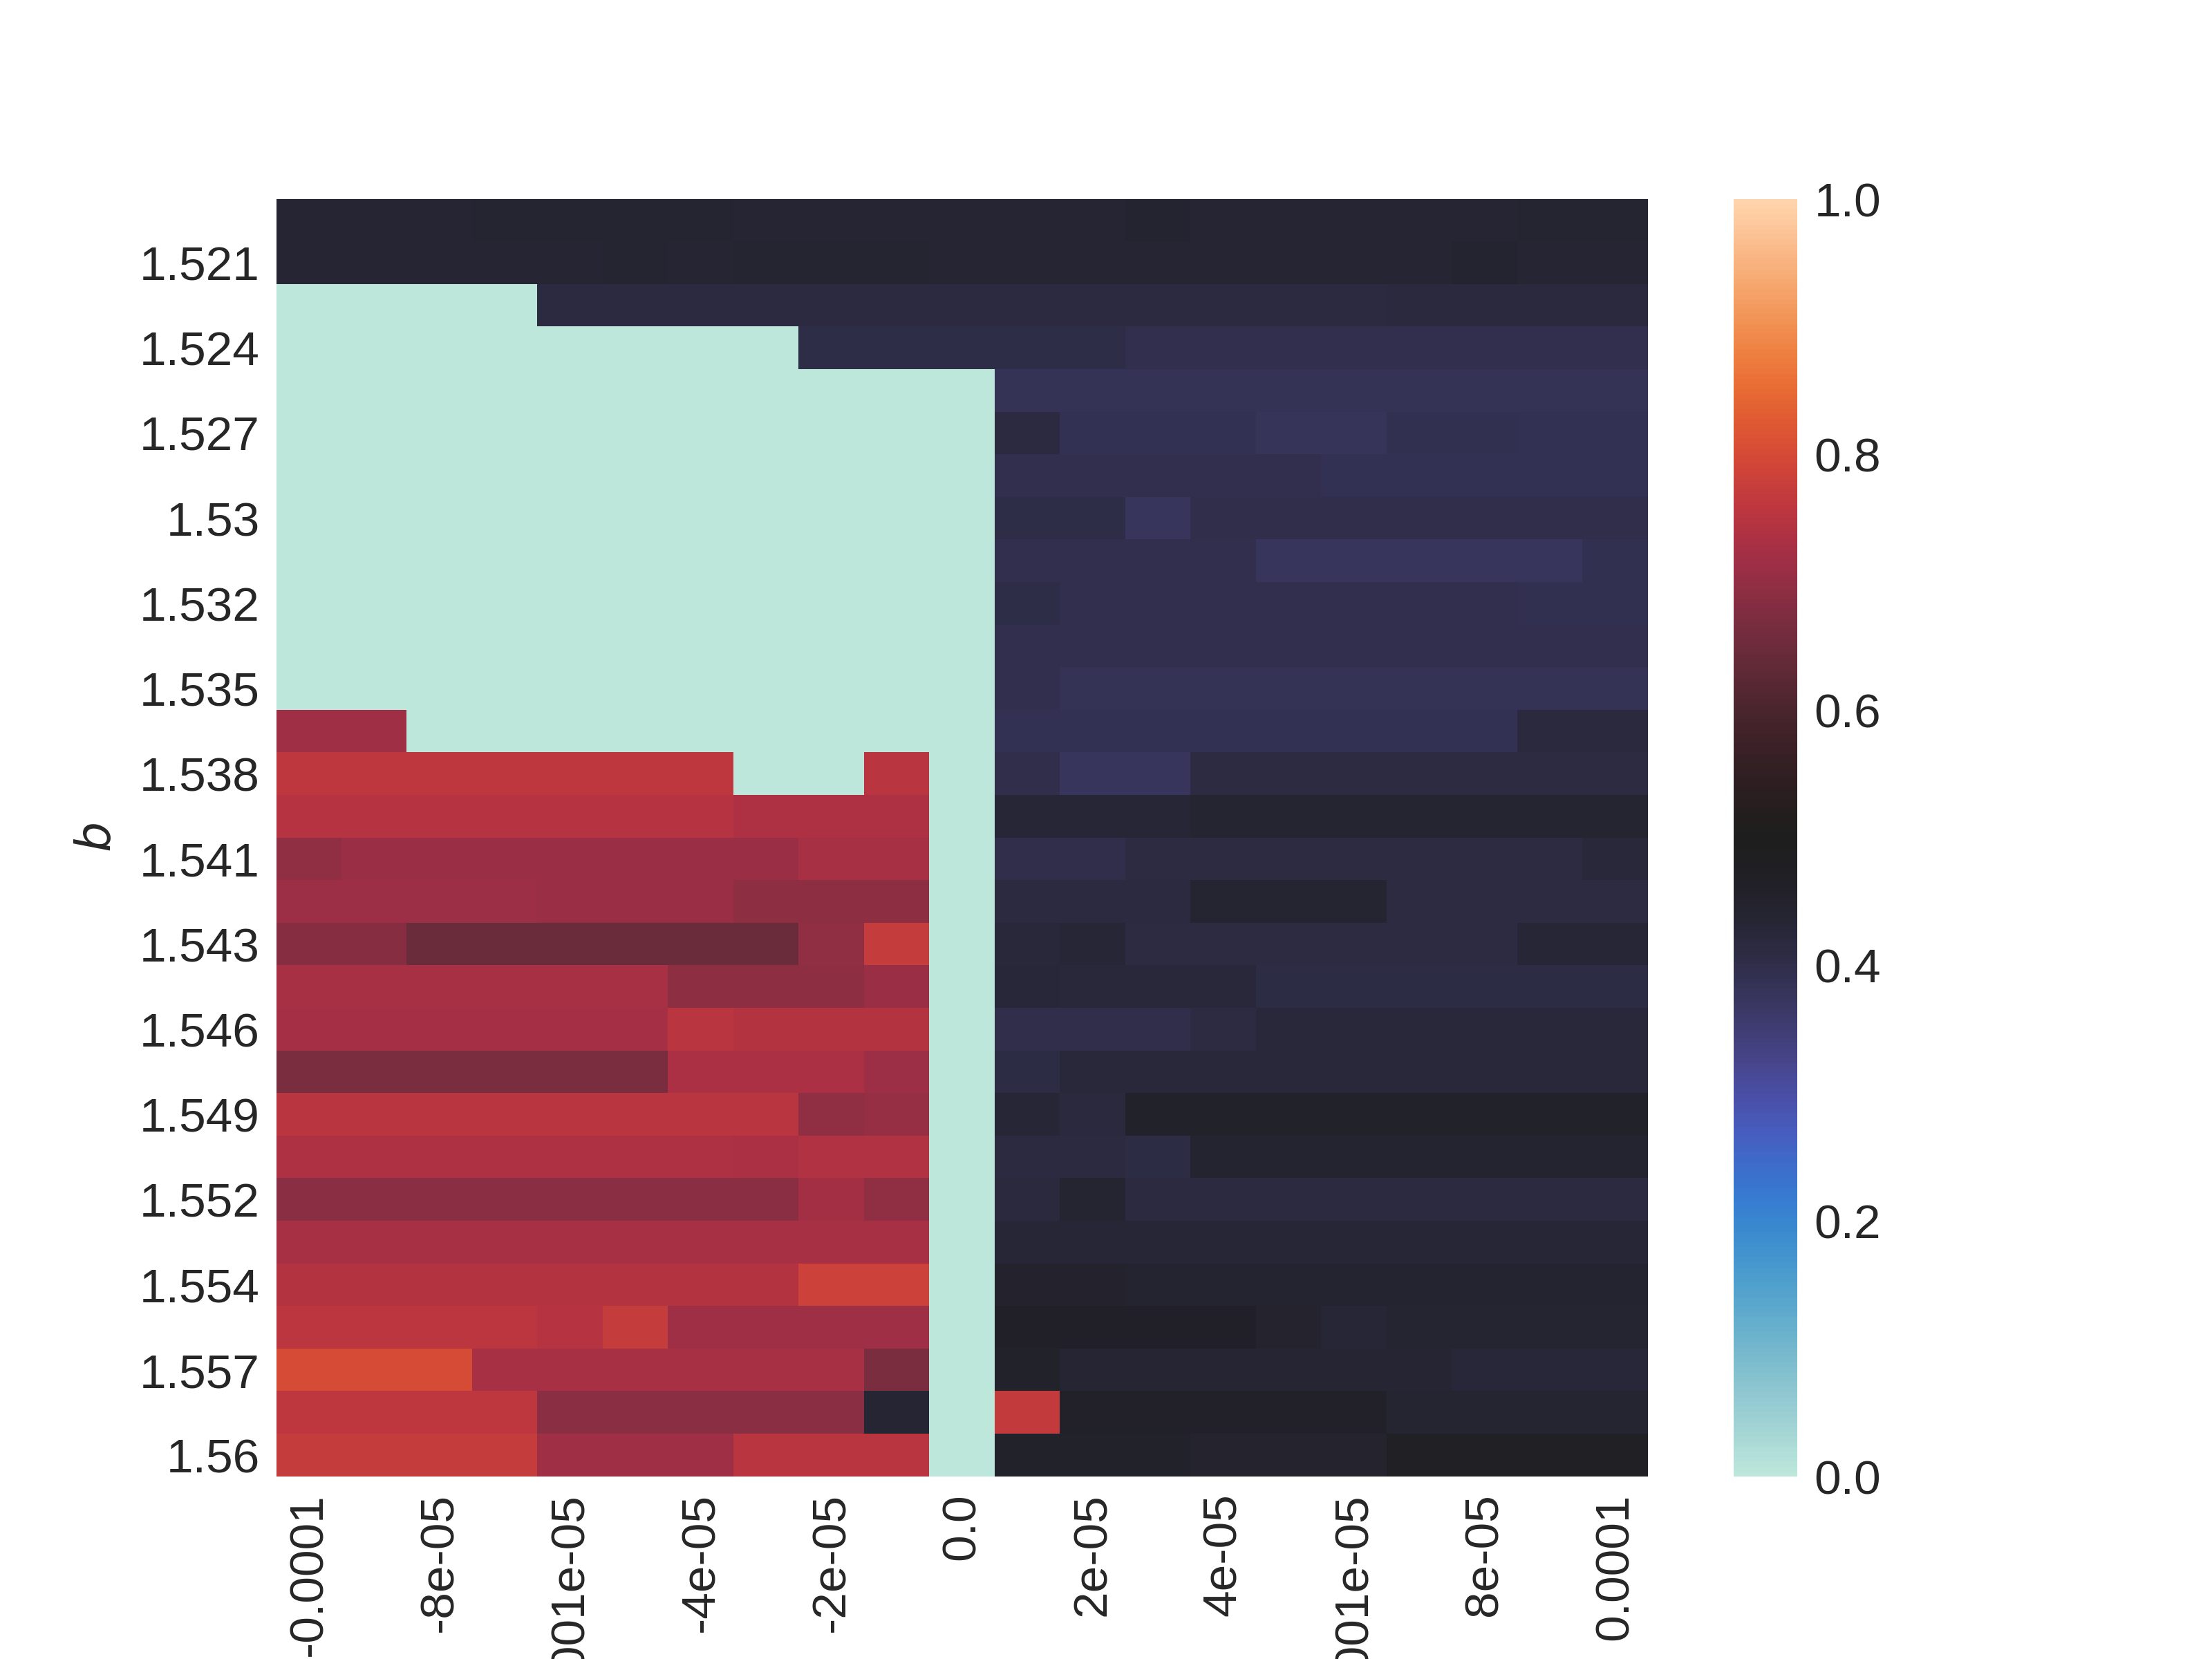
\includegraphics[width=0.95\columnwidth, keepaspectratio=True]{DoubleField/persistence_chaos_small.png}
         \caption{Persistence вблизи диагонали $(b, b)$. $\Delta$ с шагом $0.00001$}
         \label{fig:chaos_pers_small}
    \end{figure}

\subsubsection{Связанные и несвязанные поля}
    На рис. \ref{fig:chaos_compare} показано сравнение при игре на связанных и несвязных полях. Как можно видеть, при взаимодействии полей режим, в котором на втором поле хаос, становится гораздо меньше.
    На рис. \ref{fig:chaos_states} разница между двумя режимами видна еще лучше. Там где при несвязных полях оба поля находятся в состоянии хаоса, на связных полях может быть "стабильное"\footnote{Условно стабильное, так как при нашем определении для него достаточно одного не изменяющегося агента.} состояние.
    \begin{figure}[H]
         \centering
         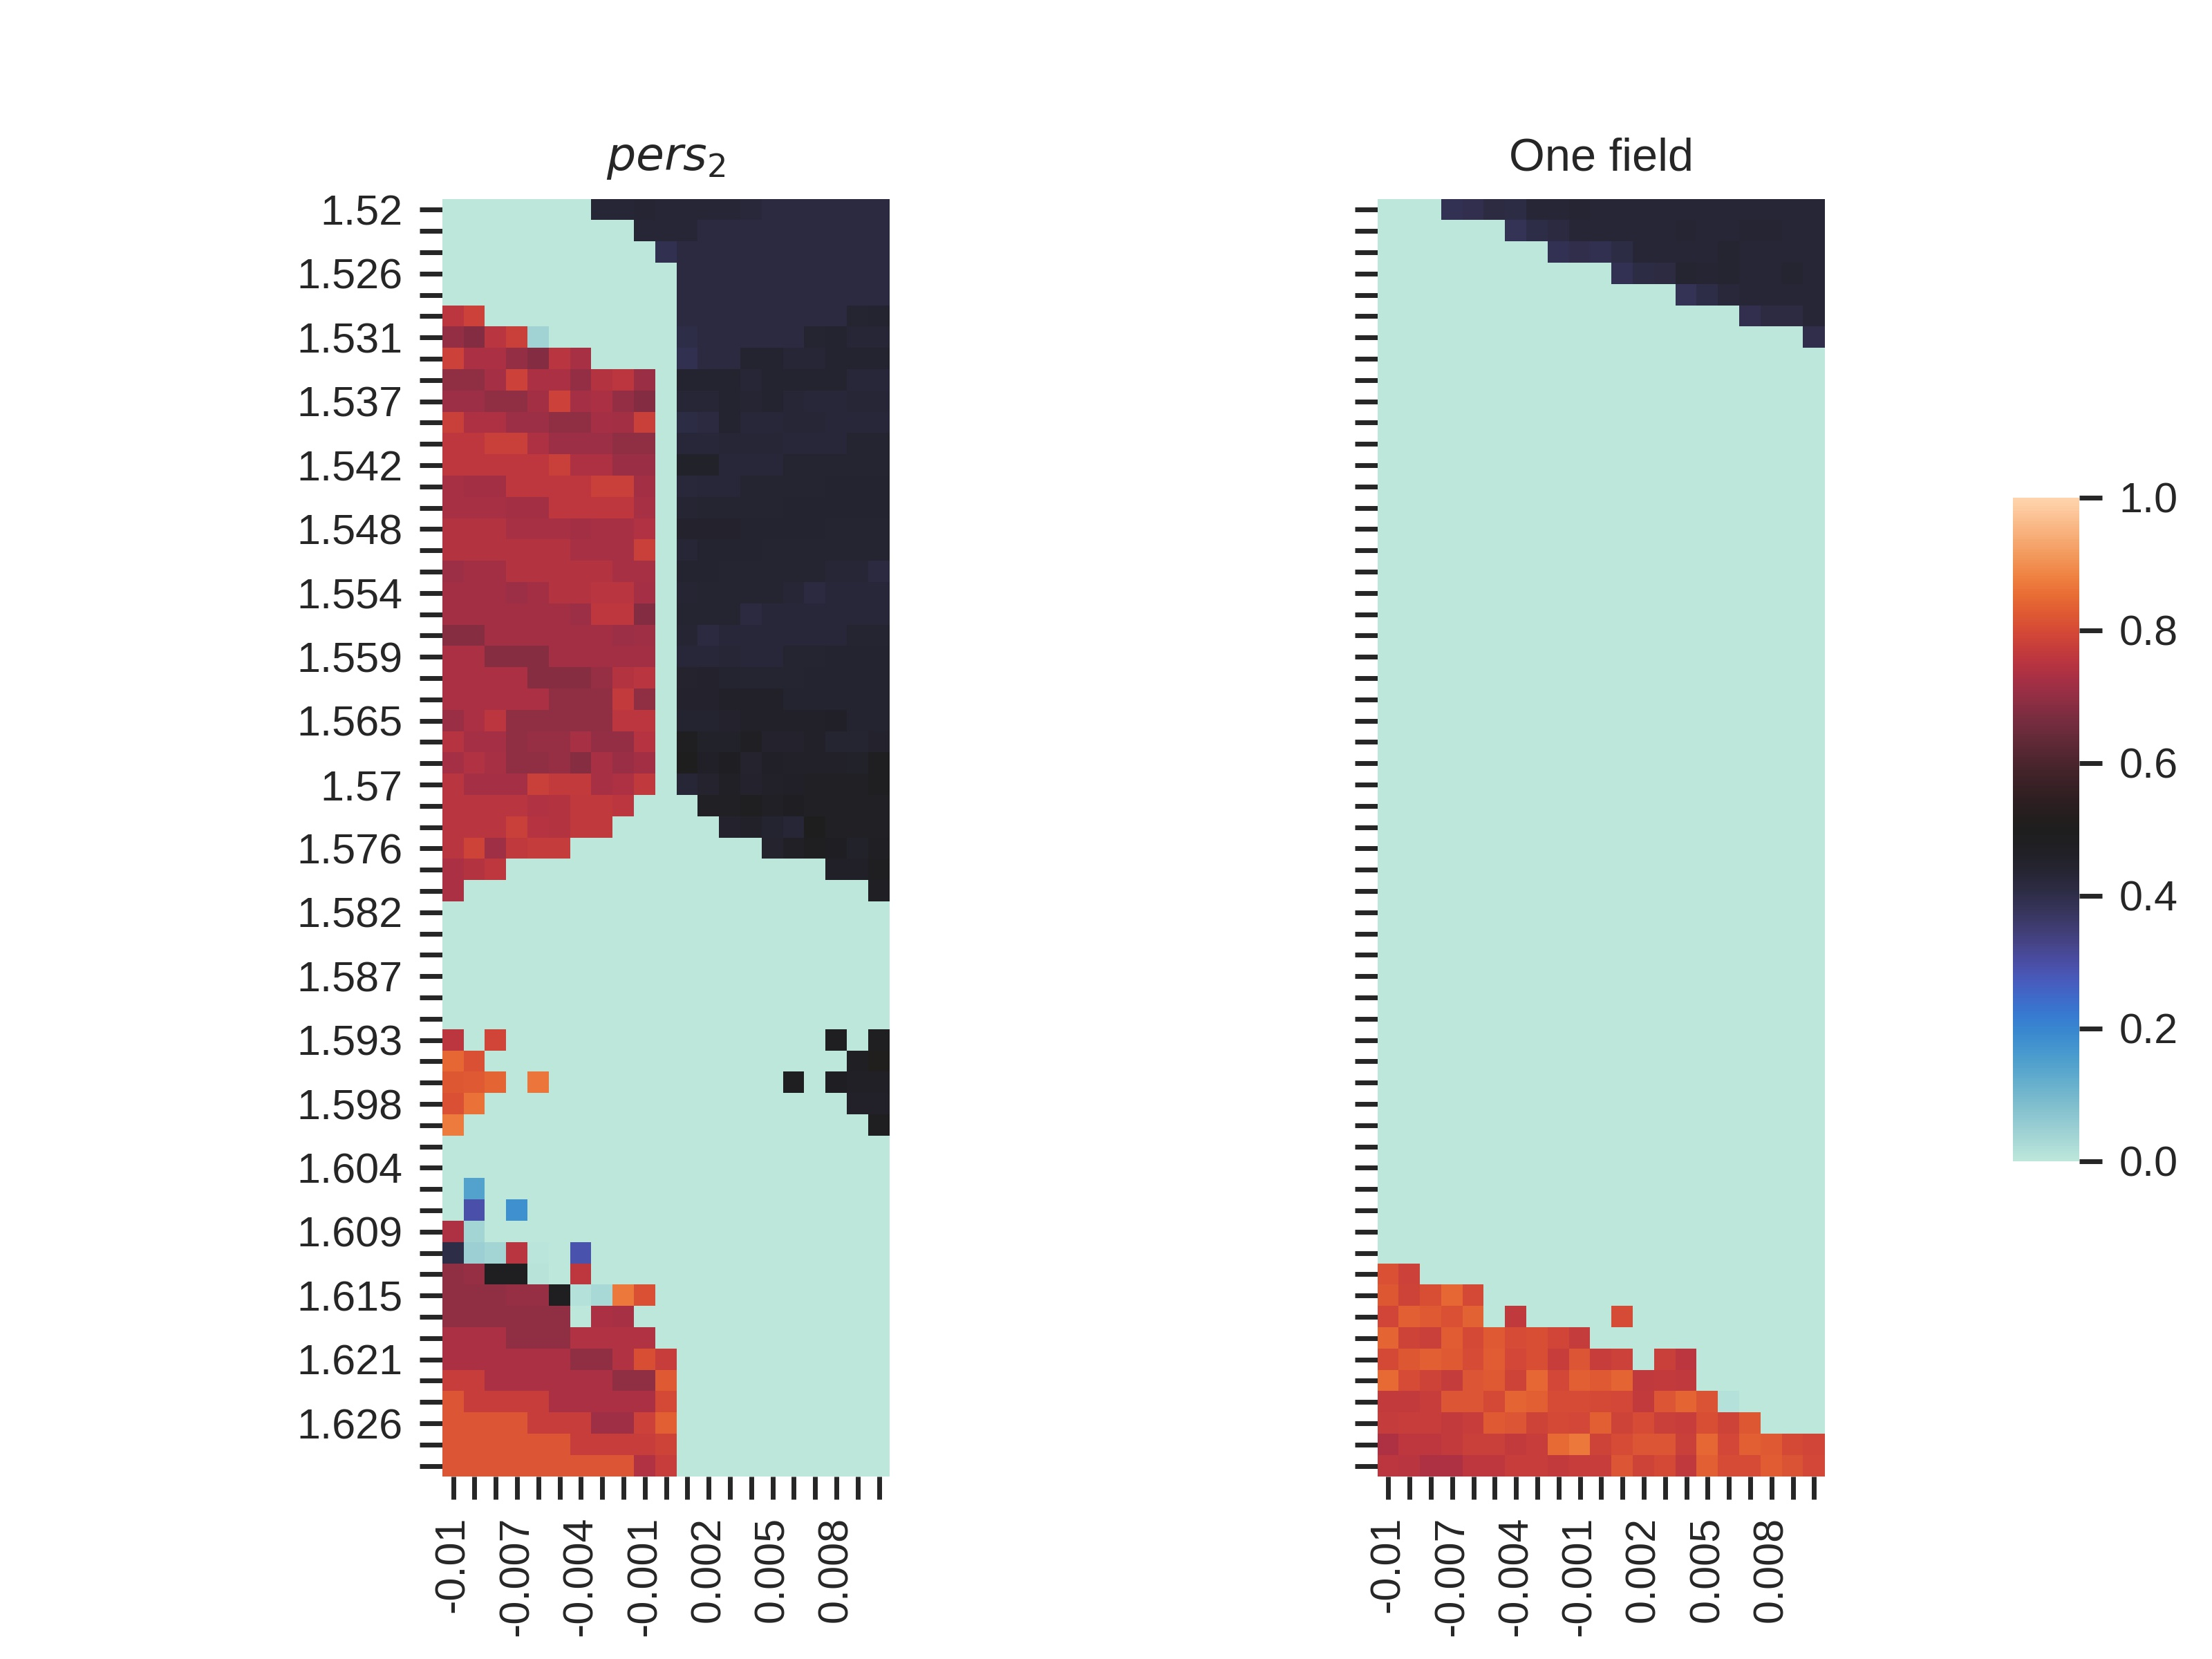
\includegraphics[width=0.95\columnwidth, keepaspectratio=True]{DoubleField/double_field_comparison_pers.jpg}
         \caption{Persistence на втором поле вблизи диагонали $(b, b)$ при игре \textbf{на связанных полях и несвязанных}. По вертикальной оси значение $b$, по горизонтали расстояние от диагонали $\Delta$ ($(b_1,\;b_2) = (b,\;b) + (1/\sqrt{2},\;-1/\sqrt{2})\Delta$). Цветом обозначен $persistence$. $\Delta$ с шагом $0.001$}
         \label{fig:chaos_compare}
    \end{figure}
    
    \begin{figure}[H]
         \centering
         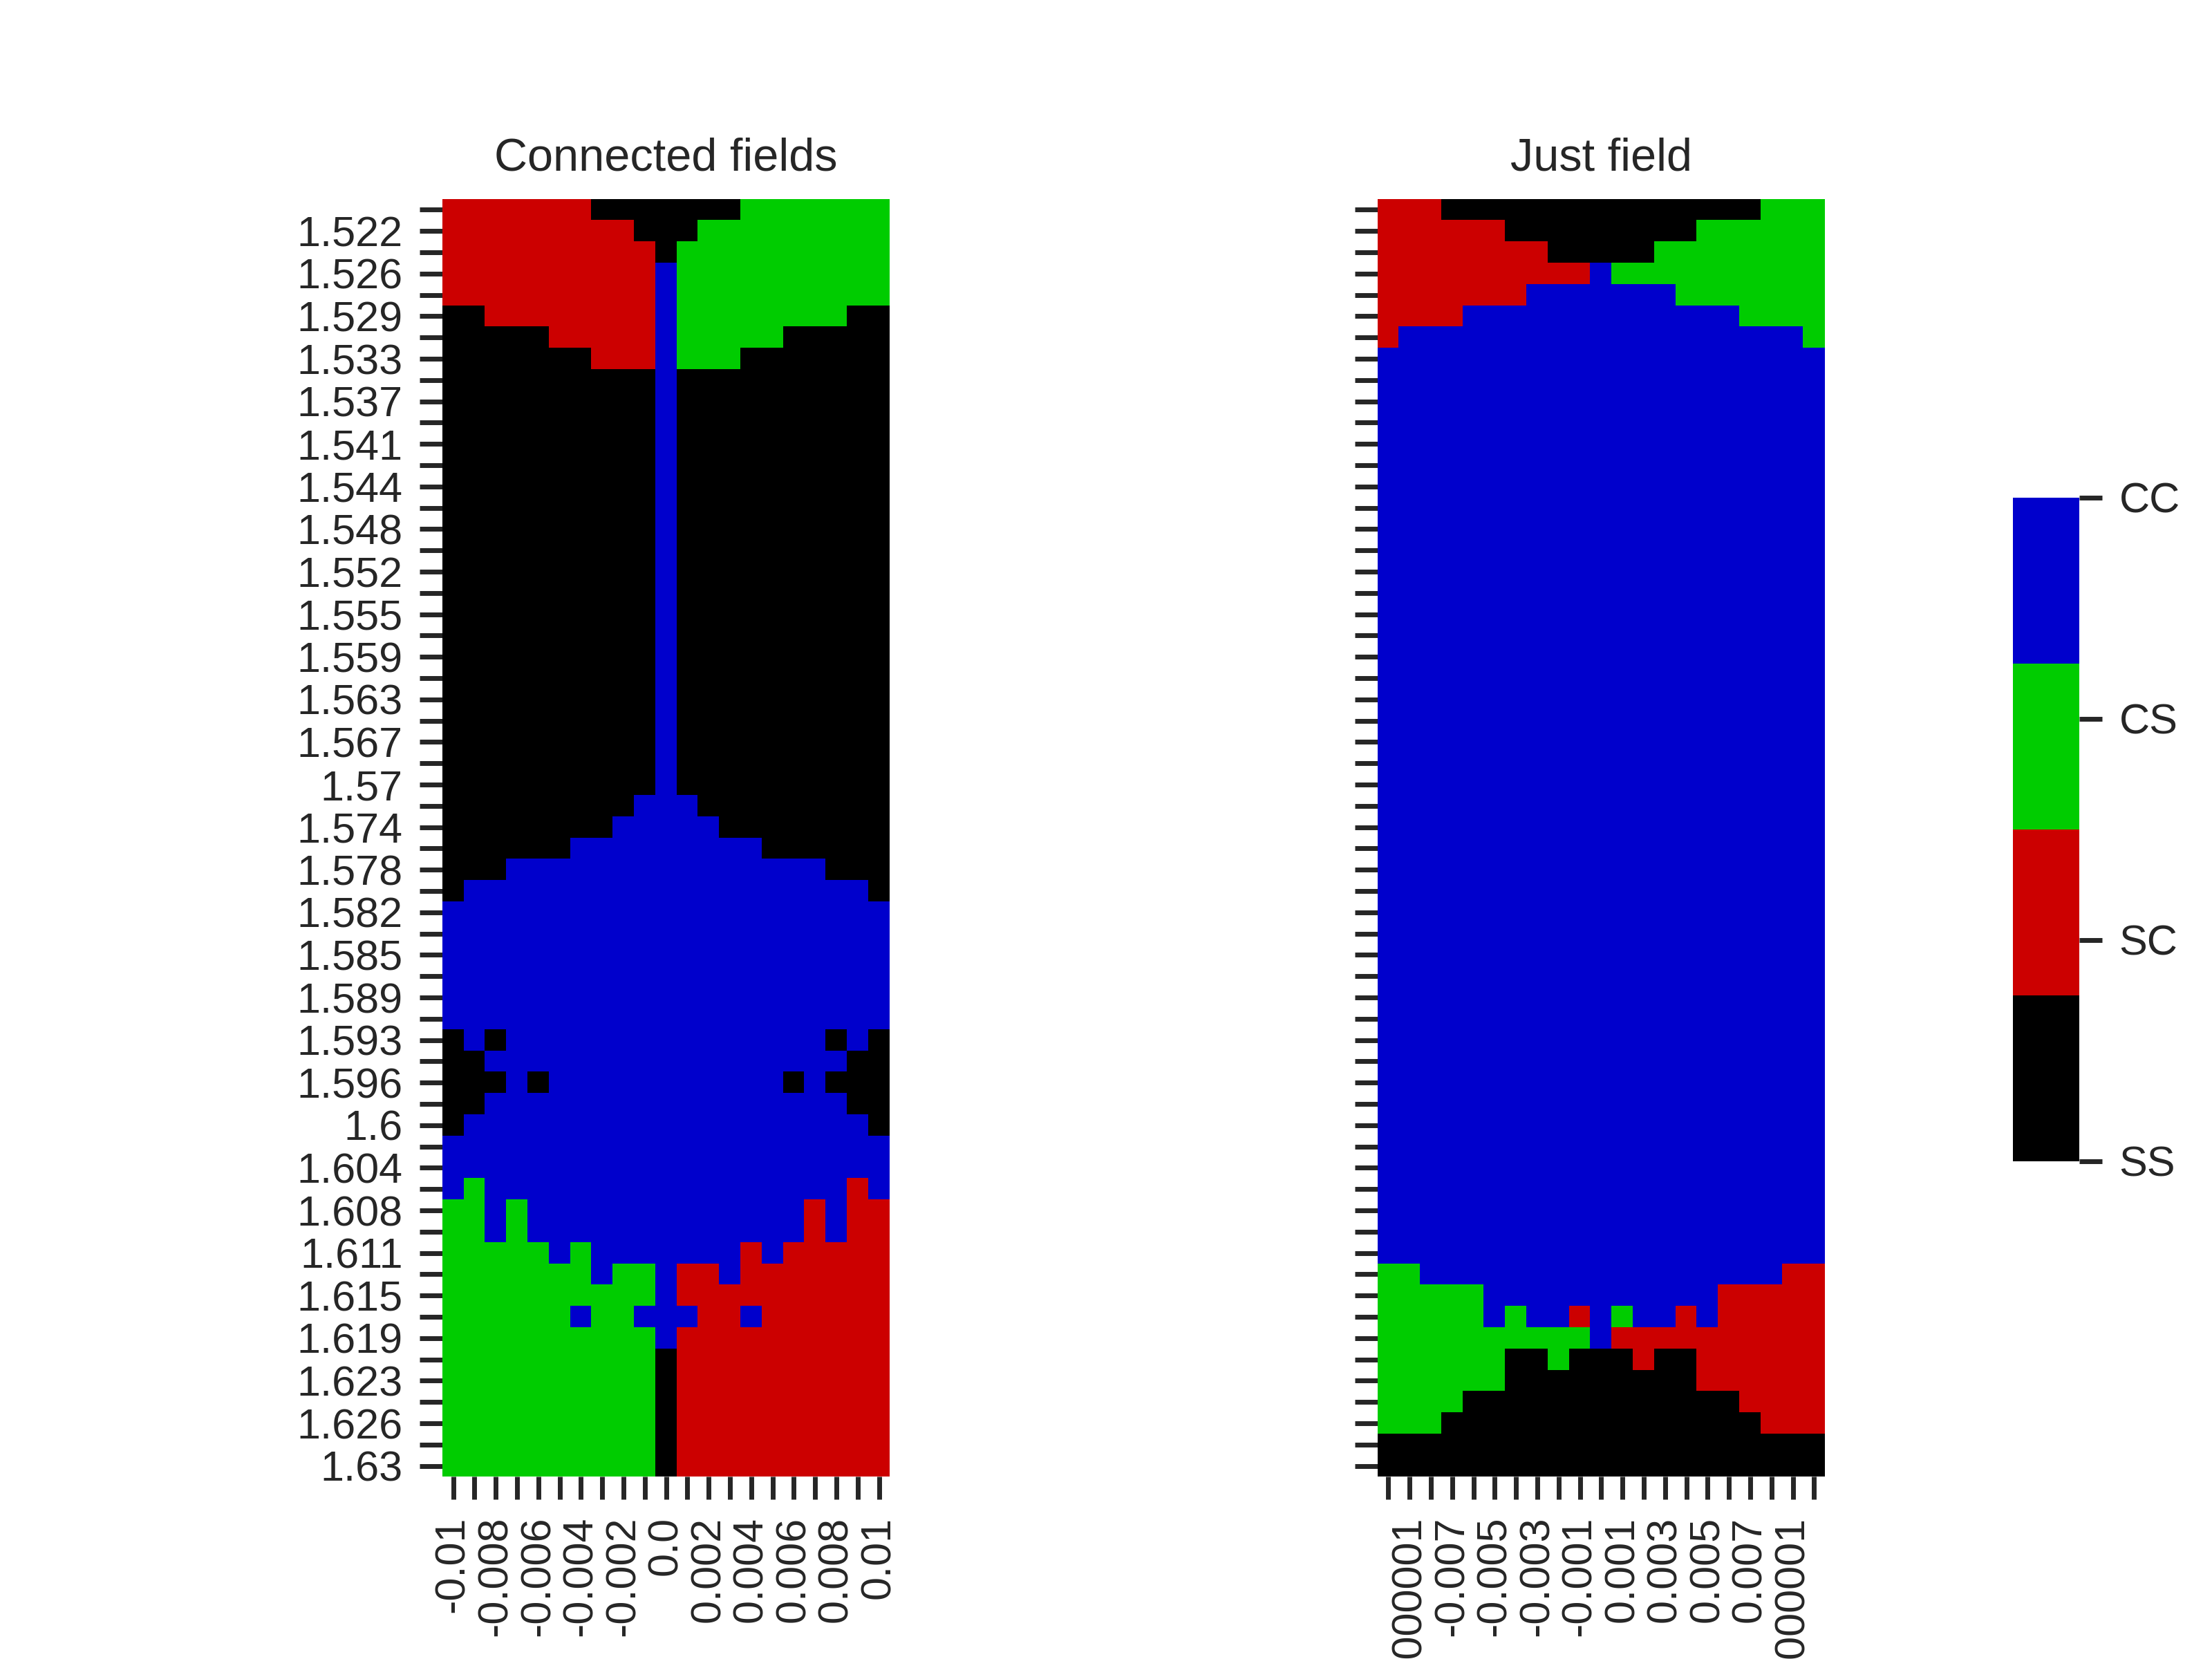
\includegraphics[width=0.95\columnwidth, keepaspectratio=True]{DoubleField/double_field_state_comparasion.png}
         \caption{Состояние полей вблизи диагонали $(b, b)$ при игре \textbf{на связанных полях и несвязанных}. По вертикальной оси значение $b$, по горизонтали расстояние от диагонали $\Delta$ ($(b_1,\;b_2) = (b,\;b) + (1/\sqrt{2},\;-1/\sqrt{2})\Delta$). $\Delta$ с шагом $0.001$\\
         Синий - хаос на обоих полях\\
         Зеленый - хаос на втором поле\\
         Красный - хаос на первом поле\\
         Черный - отсутствие хаоса на обоих полях}
         \label{fig:chaos_states}
    \end{figure}
    
\subsection{Конфигурации поля}
    Так как существуют значения $(b_1, b_2)$ при которых persistence не 0 и не 1 одновременно, было интересно посмотреть на конфигурации при различных значениях выигрыша. На рис. \ref{fig:Dfields} показаны конфигурации поля на большом времени при $b_1,\;b_2\in\{0.9, 1.24, 1.4, 1.55, 1.7, 1.98\}$. Предварительно нельзя говорить о появлении каких-либо новых конфигураций по сравнению с обычной игрой со средним полем.
    \begin{figure}[H]
         \centering
         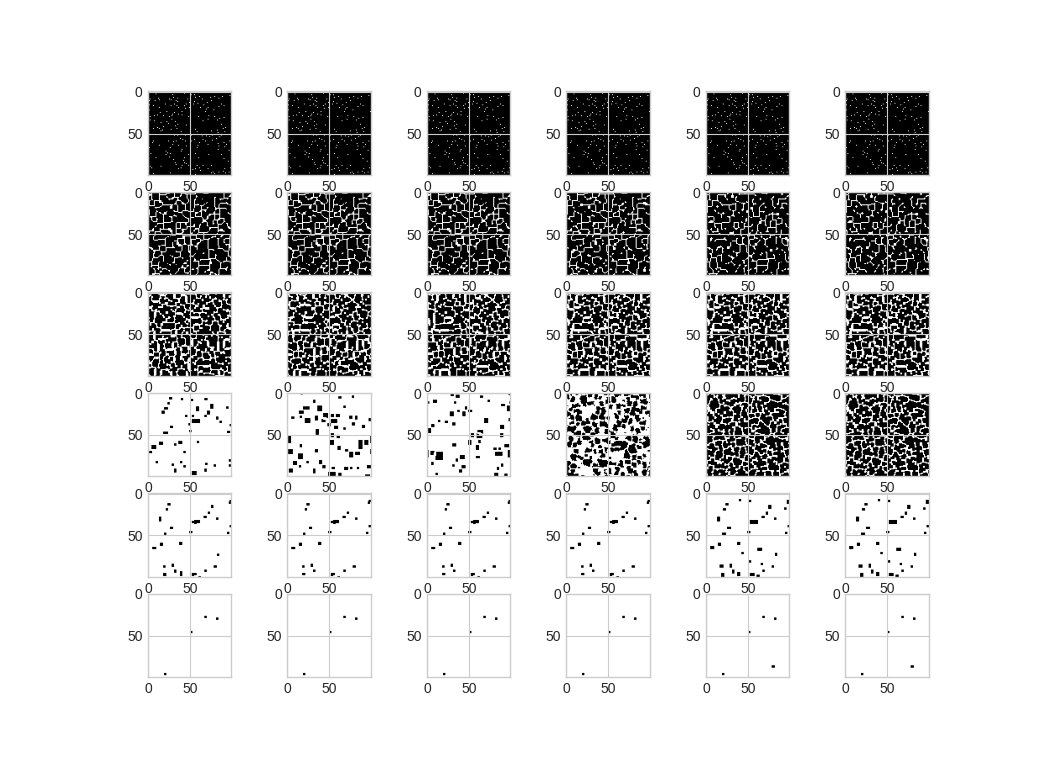
\includegraphics[width=0.95\columnwidth, keepaspectratio=True]{DoubleField/differentconfigs.png}
         \caption{Конфигурации поля.}
         \label{fig:Dfields}
    \end{figure}
    
    \begin{figure}
         \centering
         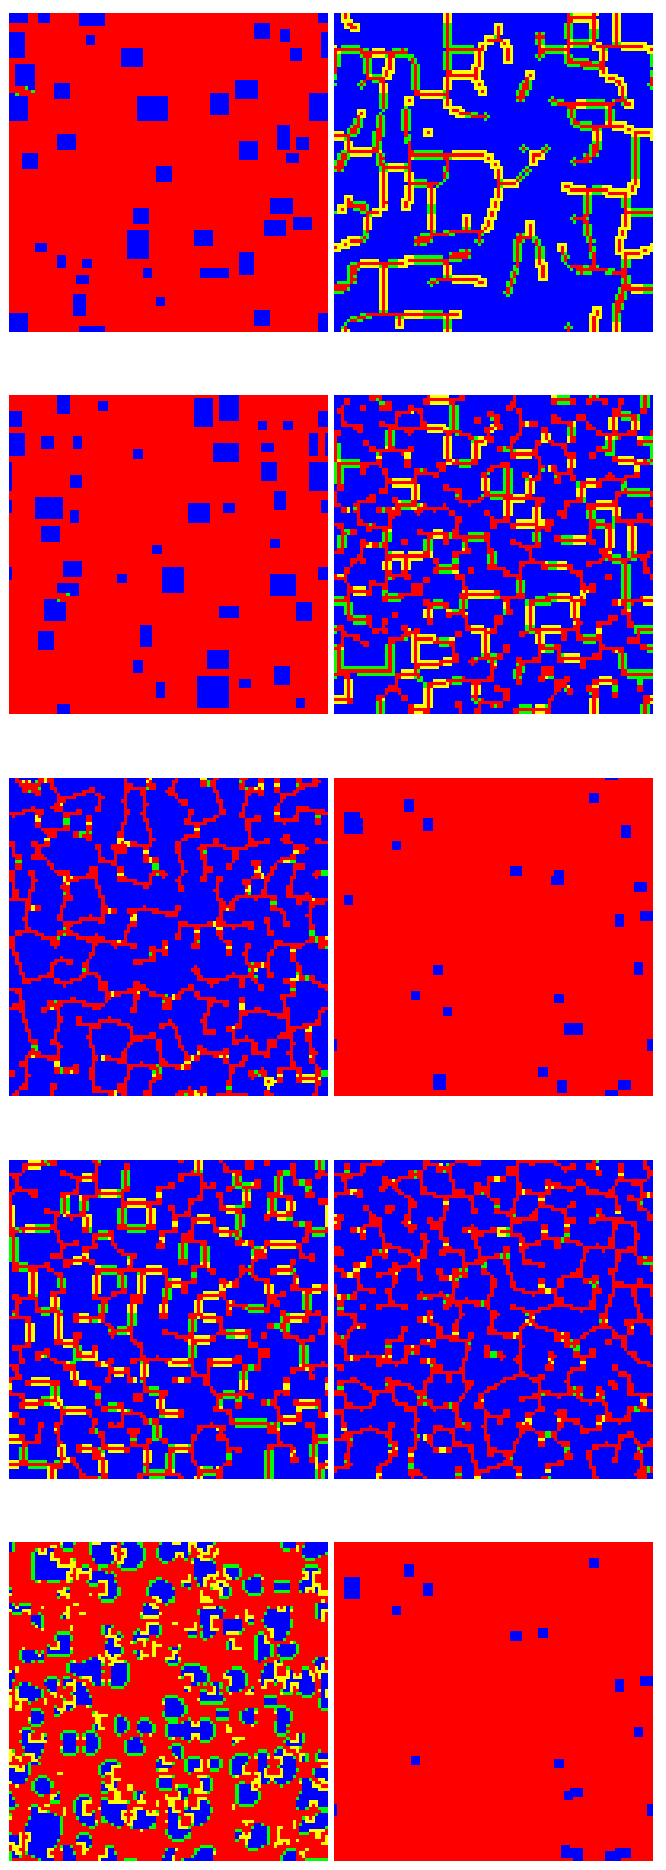
\includegraphics[width=0.5\columnwidth, keepaspectratio=True]{DoubleField/colored_2fields.png}
         \caption{Окрашенные поля при $((1.53, 1.38),
          (1.56, 1.46),
          (1.56, 1.7),
          (1.37, 1.46),
          (1.6, 1.8))$.}
         \label{fig:colfields}
    \end{figure}

\subsubsection{Еще пример изменения конфигураций}
    \label{sec:configs}
    На рис. \ref{fig:fields156} показаны поле 1 и 2 при различных значениях $b_2$. Как видно из рисунка, при $b_2\neq b_1$, на обоих полях наблюдаются устойчивые конфигурации, причем при $b_2<b_1$, на первом поле кооператоры образуют прямоугольные кластеры, а на втором дефекторы образуют сеть каналов с крупными кластерами кооператоров. При $b_2=b_1$ на обоих полях агенты находятся в хаотическом режиме.
    \begin{figure}
         \centering
         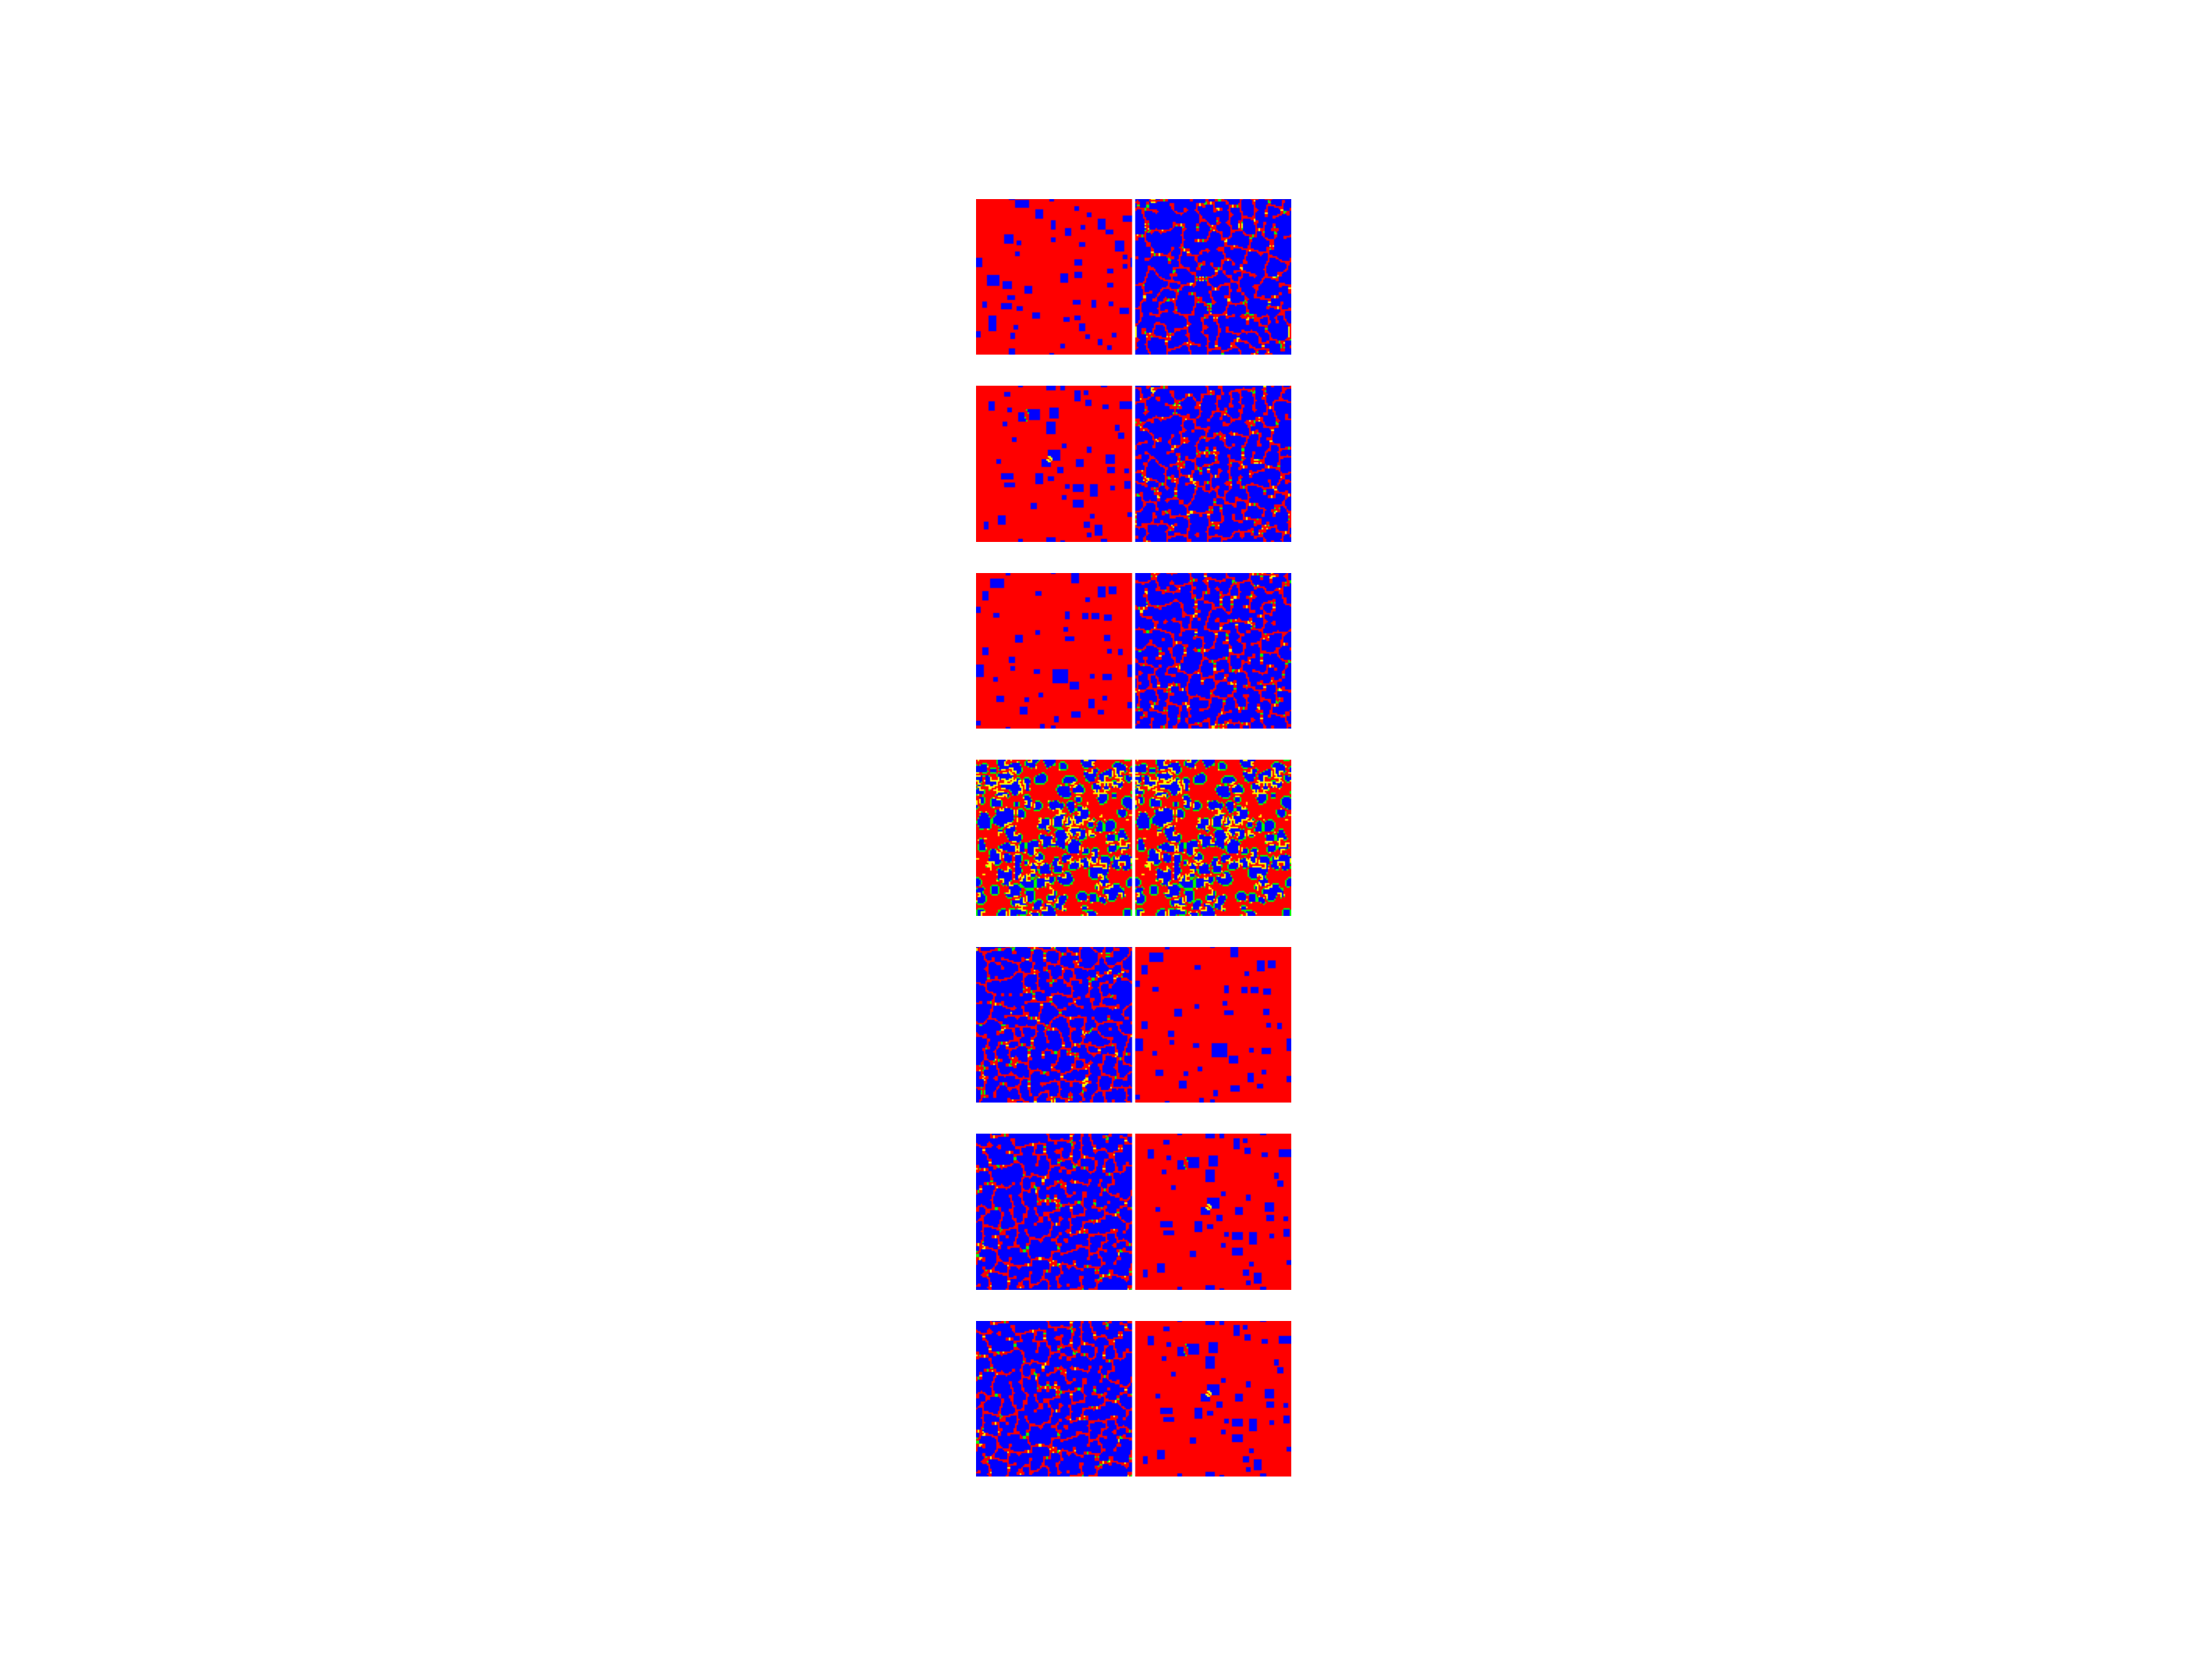
\includegraphics[width=0.95\columnwidth, keepaspectratio=True]{DoubleField/colored_2fields156.png}
         \caption{Окрашенные поля при $b_1=1.56$ и $b_2=1.557, 1.558, 1.559, 1.56, 1.561, 1.562, 1.563$}
         \label{fig:fields156}
    \end{figure}

\newpage
\begin{thebibliography}{9}
    \bibitem{NACHBAR1992307}
        John H. Nachbar, \textit{Evolution in the finitely repeated prisoner's dilemma}, Journal of Economic Behavior \& Organization \textbf{19}(3), 307(1992).
    
    \bibitem{NOWAK1992}
        Martin Nowak and Robert May, \textit{Evolutionary games and spatial chaos}, Nature \textbf{359}(10), 826(1992).

    \bibitem{NOWAK1993}
        Martin Nowak and Robert May, \textit{The spatial dilemmas of evolution}, International Journal of Bifurcation and Chaos \textbf{03}(01), 35(1993).

    \bibitem{KOLOTEV2018}
        Sergei Kolotev, Aleksandr Malyutin, Evgeni Burovski, Sergei Krashakov, and Lev Shchur, \textit{Dynamic fractals in spatial evolutionary games}, Physica   A:   Statistical   Mechanics and its Applications \textbf{499}, 142(2018).
\end{thebibliography}
\end{document}